\documentclass[twoside,11pt]{article}
\setlength{\parskip}{0pt} % No space between paragraphs
\usepackage{texstyle}
\usepackage{setspace}
\onehalfspacing % Line space
\usepackage{mathtools} % vertical centered colon (vcentcolon)
\usepackage{amsmath} % For \argmax
\DeclareMathOperator*{\argmax}{argmax} % thin space, limits underneath in displays
\usepackage{lineno}

\usepackage{subdepth} % subscript would be at the same height no matter whether there is a superscript.
\usepackage{graphicx}
\usepackage{caption}
\usepackage{subcaption}
\usepackage[toc,page]{appendix}

\usepackage{bookmark}
\bookmarksetup{open,numbered}

\usepackage{tabularx}
\newcolumntype{Y}{>{\centering\arraybackslash}X}

\setlength{\marginparwidth}{2.5cm} % For notes in margin, can be delete for final version.

\newcommand{\dataset}{{\cal D}}
\newcommand{\fracpartial}[2]{\frac{\partial #1}{\partial  #2}}
\DeclareMathOperator{\Tr}{Tr}

\definechangesauthor[name={Per cusse}, color=brown]{Kungang}
\definechangesauthor[name={Per cusse}, color=orange]{Anh}
\definechangesauthor[name={Per cusse}, color=red]{Apley}

\firstpageno{1}

\begin{document}

\title{Concept Drift Monitoring and Diagnostics of Supervised Learning Models via Score Vectors}

\author{\name Kungang Zhang\textsuperscript{1} \email zkg@u.northwestern.edu \\
	\name Anh T.\ Bui\textsuperscript{2} \email buiat2@vcu.edu \\
	\name Daniel W.\ Apley\textsuperscript{1} \email apley@northwestern.edu \\
       \addr \textsuperscript{1}Department of Industrial Engineering and Management Sciences\\
       Northwestern University\\
       Evanston, IL 60208-3119, USA\\
       \textsuperscript{2}Department of Statistical Sciences and Operations Research\\ 
       Virginia Commonwealth University\\
       Richmond, VA 23284-3083, USA}

\maketitle

\begin{abstract}%   <- trailing '%' for backward compatibility of .sty file

Supervised learning models are one of the most fundamental classes of models. Viewing supervised learning from a probabilistic perspective, the set of training data to which the model is fitted is usually assumed to follow a stationary distribution. However, this stationarity assumption is often violated in a phenomenon called concept drift, which refers to changes over time in the predictive relationship between covariates $\bm{X}$ and a response variable $Y$ and can render trained models suboptimal or obsolete. We develop a comprehensive and computationally efficient framework for detecting, monitoring, and diagnosing concept drift. Specifically, we monitor the Fisher score vector, defined as the gradient of the log-likelihood for the fitted model, using a form of multivariate exponentially weighted moving average, which monitors for general changes in the mean of a random vector. In spite of the substantial performance advantages that we demonstrate over popular error-based methods, a score-based approach has not been previously considered for concept drift monitoring. Advantages of the proposed score-based framework include applicability to any parametric model, more powerful detection of changes as shown in theory and experiments, and inherent diagnostic capabilities for helping to identify the nature of the changes.
\end{abstract}

\begin{keywords} 	
  Concept Drift, Score Function, Control Chart, Predictive Model, Multivariate EWMA
\end{keywords}

\section{Introduction}
\label{s_CD:intro}
In supervised learning, models are trained to predict a response variable $Y$, given an observed set of covariates $\bm{X} \in \mathbb{R}^p$. The modeling goal is usually to make test prediction accuracy metrics~(i.e., $R^2$, classification accuracy, F1-score, etc.) as high as possible. A supervised learning model can also act as an intermediate module in other machine learning tasks, such as dimension reduction in unsupervised learning or Q-Learning in reinforcement learning. Training a supervised learning model can be viewed as an optimization problem. From a probabilistic perspective, a training sample of observations, $\{\bm {x}_i, y_i\}_{i=1}^n$, is usually assumed to be drawn from some joint distribution, $P (\bm {X}, Y)$, such that the conditional distribution, $P(Y|\bm{X};\bm{\theta})$, is stationary across the $n$ observations~(\cite{hulten2001mining}). Here, {$\bm {x}_i \in \mathbb{R}^{p}$ and $y_i \in \mathbb{R}$ are the covariates and response variable in the $i$th observation respectively}\footnote{The case with scalar response can easily be extended to a vector response variable $\bm {y}_i$.}, and we have parametrized the conditional distribution via the vector $\bm{\theta}$. However, the stationarity assumption is often violated in real applications, a phenomenon known as concept drift~(\cite{moreno2012unifying,vzliobaite2016overview}). For example, models used to predict customers' probabilities of defaulting by credit-scoring agencies are usually fitted to training data collected over a three to five years period, so that changing financial environments may result in a partially-outdated predictive relationship by the time the trained model is used to score new customers~(\cite{crook1992degradation,vzliobaite2016overview}). 

Concept drift poses many challenges in constructing trustworthy supervised learning models. Concept drift during training~(for historical data) and testing/usage~(for future data) both can degrade performance of supervised learning models: during training, concept drift results in there being no single predictive model, since the model is changing over time; while concept drift during testing/usage degrades the accuracy of the predictive model, relative to what it could be with an updated model for $P(Y|\bm{X};\bm{\theta})$. In order to obtain and maintain the highest possible predictive performance of supervised learning models, \textit{retrospective} concept drift analysis~(see Figure~\ref{fig_CD:proc_mon_score_retro} and corresponding descriptions) of the training data and \textit{prospective} concept drift monitoring of the test data~(see Figure~\ref{fig_CD:proc_mon_score_monitoring} and corresponding descriptions) are important and should be a standard component of the predictive modeling process.

Concept drift is common in practice and often originates from changes of some hidden effects in generating the response outcomes of interests~(\cite{tsymbal2008dynamic,vzliobaite2012beating,widmer1996learning,kukar2003drifting,donoho2004early,carmona2010gnusmail,harel2014concept,fong2015change,vzliobaite2016overview}). For example, in the problem of antibiotic resistance in nosocomial infections, supervised learning models are trained and validated using a data set, with response labels indicating whether the level of sensitivity of a pathogen to an antibiotic is sensitive, resistant, or intermediate, and the covariates being patients' demographical data and conditions of hospitalization~(\cite{pechenizkiy2005knowledge}). After properly training and validating such a model, it can with high accuracy determine whether or not a pathogen is sensitive to an antibiotic or not. However, according to medical experts~(\cite{kukar2003drifting}), hidden effects due to failures and/or replacements of some medical equipment, changes in personnel, and seasonal bacterial outbreaks could result in unexpected changes over time in resistance of new pathogen strains to antibiotics. In other words, there is likely a significant level of concept drift in nosocomial infections. Consequently, bacteria that are predicted to be sensitive to a particular antibiotic may now be resistant, and the errors of the predictive model becomes unacceptable. 

The problem of concept drift is gaining increasing attention, because increasingly data are organized in the form of data streams, and it is often unrealistic to expect that data distributions remain stable for a long period of time. Most state-of-the-art concept drift detection and adaptation methods, like ensemble methods~(\cite{wang2003mining}), neural networks~(\cite{calandra2012learning}), and other non-parametric methods~(\cite{bifet2007learning,frias2015online}), are based on monitoring the classification error or some metrics derived from it~(\cite{ross2012exponentially,gonccalves2014comparative,barros2018large}). 

The main purpose of this paper is to introduce a new and comprehensive concept drift framework that is based on monitoring the Fisher scores of the individual observations over time, as opposed to metrics derived from their classification errors. The Fisher score, which we will refer to as simply the score, of an observation $(\bm{X}, Y)$ is defined as the gradient of the log-likelihood, $\log{P(Y|\bm{X};\bm{\theta})}$, with respect to the parameters, $\bm{\theta}$. As shown in the following sections, comparisons between the score-based and error-based methods from both theoretical and empirical perspectives provide strong justification for a score-based approach. The score-based framework that we develop and demonstrate is intended to detect, monitor, and diagnose concept drift with the following major advantages and attractive properties.

\begin{itemize}
\item
\textit{The approach is based on monitoring for changes in the mean of the score vector, which has strong theoretical justification since theory dictates that the mean of the score vector changes if and only if $P(Y|\bm{X};\bm{\theta})$ changes, under fairly general conditions~(Section~\ref{ss_CD:score_func}).}
\item
\textit{In contrast, existing concept drift methods that are based on monitoring the error rate may fail to detect concept drift, because a change in $P(Y|\bm{X};\bm{\theta})$ does not necessarily result in an increase~(or a decrease) in the error rate~(see Section~\ref{ss_CD:score_func}). Note that a change in $P(Y|\bm{X};\bm{\theta})$ that does not change the error rate still means that, if the model is updated accordingly after concept drift detection, the predictive accuracy of the model can be improved~(Section~\ref{ss_CD:cd_no_err_change}). Thus it is still desirable to detect such changes.}
\item
\textit{The score-based approach is more sensitive to changes in $P(Y|\bm{X}; \bm{\theta})$ and thus more quickly detects concept drifts than error-based methods, as demonstrated empirically with a number of examples~(Section~\ref{s_CD:real_data} and Appendices~\ref{app:simu_MRL} and~\ref{app:cd_diag}).}
\item
\textit{The score-based approach is applicable to any parametric classification or regression model that can be interpreted probabilistically in terms of $P(Y|\bm{X};\bm{\theta})$, parameterized by a vector of parameters $\bm{\theta}$.}
\item
\textit{The score-based approach also naturally provides a convenient means of diagnosing the nature of the concept drift~(e.g., which parameters have changed) as derived in Section~\ref{s_CD:decou_cd} and demonstrated in Section~\ref{s_CD:real_data} and Appendix~\ref{app:cd_diag}.}
\item
\textit{The score-based perspective converts the concept drift problem to the problem of monitoring changes in the mean of a random vector, for which many existing multivariate statistical process control~(SPC) methods are available. We focus on a multivariate exponentially weighted moving average~(MEWMA) control chart~(\cite{lowry1992multivariate,hotelling1947multivariate,montgomery2007introduction}), which has desirable characteristics for our problem~(see Section~\ref{ss_CD:MEWMA}), but as new methods are developed they can also be applied.}
\item
\textit{The computations involved in the score-based approach are almost the same computations involved in stochastic gradient descent~(SGD) algorithms, which are increasingly commonly used to fit parametric supervised learning models. In this sense, the computations come at very little additional cost, resulting in a computationally inexpensive approach~(Section~\ref{ss_CD:sgd_score}).}
\item
\textit{The same score-based concepts can be used in a consistent manner either retrospectively~(e.g., after fitting a supervised learning model to a set of training data, to validate that the training data were stable and, if not, provide diagnostic information as to why) or prospectively~(e.g., when using a fitted supervised learning model to predict new cases, to quickly signal when the predictive model has changed, indicating that it is time to update the model).}
\end{itemize}

We elaborate on these properties in Sections~\ref{s_CD:theory_analysis_score} and~\ref{s_CD:decou_cd} and provide simulation results demonstrating them in Appendices~\ref{app:simu_MRL} and~\ref{app:cd_diag}. Two real examples (credit risk scoring and bike sharing demand prediction) in Section~\ref{s_CD:real_data} serve as case-studies to further illustrate its usage.

\section{Relation to Prior Work}
\label{s_CD:review}
In this section, we briefly review relevant existing literature on monitoring different types of drift in data distributions, in terms of goals and methodologies. The impact of the drift on model training and prediction depends on the particular type of drift. In the literature on data set drift, the terminology is not always consistent. In this work, we follow what appears to be the most common terminology according to~\cite{moreno2012unifying} and~\cite{vzliobaite2016overview}. In general, any temporal drift in the joint distribution $P(\bm {X}, Y)$ is called ``data set drift". Decomposing the joint distribution as $P(\bm{X}, Y) = P(Y|\bm{X})P(\bm {X})$, the term ``concept drift" refers to temporal drift in $P(Y|\bm{X})$~(which is what the fitted supervised learning model approximates), while ``covariate drift" refers to temporal drift in $P(\bm{X})$.

In general, the methods in the concept drift literature can be categorized into two classes~(\cite{tsymbal2004problem,harel2014concept}): 1) model adaptation methods and 2) concept drift detection methods. Model adaptation methods mainly focus on maintaining the performance of machine learning models in the presence of concept drift, without formally detecting or diagnosing the drift~(\cite{wang2003mining,tsymbal2008dynamic,gonccalves2014comparative,barros2018large}). To maintain a good prediction metric related to classification or regression error, models are automatically updated~(i.e., adapted) online continuously as new observations are collected, which is sometimes called online or incremental learning. This class of methods is not particularly relevant to our work, since our goal is concept drift detection and diagnosis, and not model adaptation. In fact, we view our approach as something that can be used in conjunction with model adaptation methods to make them more efficient and interpretable. In particular, the model adaptation could be turned on only when the concept drift detection component has indicated that $P(Y|\bm{X};\bm{\theta})$ has changed. This would avoid unnecessarily adapting the model when $P(Y|\bm{X}; \bm{\theta})$ is stable, which is counterproductive in terms of both predictive performance and computational expense. Alternatively, in some applications in which the model adaptation component must run continuously, our score-based concept drift detection component could be run concurrently to provide diagnostic information at little additional cost.

The concept drift detection methods are more relevant to our work, and examples in this category include DDM~(\cite{gama2004learning}), EDDM~(\cite{baena2006early}), ECDD~(\cite{ross2012exponentially}), and Linear-4-rate~(\cite{wang2015concept}), etc. Although most of these methods were originally proposed in a continuous model adaptation setting, we focus on their use and performance in our setting, in which one has a single fixed model fitted to one set of training data and applies it to a test data set without updating it, so that small and gradual concept drift can be more easily detected. The drift detection method~(DDM) monitors the accumulated classification error rate as it evolves over time. The early drift detection method~(EDDM) instead monitors the intervals between consecutive errors. The EWMA for concept drift detection~(ECDD) method monitors the misclassification rate using a univariate EWMA control chart. In the Linear-4-rate method, four statistics are monitored simultaneously to detect concept drift in binary classification problems. When the particular statistic monitored in each method crosses a specified threshold, an alarm is triggered indicating that concept drift has been detected. Following an alarm, subsequent actions such as updating the model or inspecting the data sources can be taken. Most of the methods are designed specifically for binary classification and based on simple error-based quantities, like classification error, precision, recall, and residuals of the classification model~(\cite{wang2015concept,barros2018large}). As we demonstrate throughout the paper, our score-based approach is far more powerful than error-based approaches.

Although the concept drift community seems to be unaware of the potential of score-based approaches for concept drift~(e.g., it is not mentioned in the recent surveys in~\cite{barros2018large} and~\cite{lu2018learning}), there have been some works in the econometrics literature that have used the score vector to test for changes in the parameters of regression models~(\cite{kuan1995generalized,zeileis2005unified,zeileis2007generalized,xia2009monitoring}). Our work differs from this prior work in that we develop a comprehensive framework for and investigate issues more relevant in the typical situations to which the so-called concept drift paradigm refers. The econometrics work is developed mainly around the change-point paradigm in which it is assumed there is a single point in time at which $\bm{\theta}$ changes from some before-value to some after-value, and the goal is to identify the change point with formal hypotheses testing. In contrast, our approach is developed around the much more general and flexible situation in which $\bm{\theta}$ can continuously drift and/or change abruptly at multiple change-points, which is far more common in typical concept drift applications. Ours is more of an exploratory approach to inform the predictive modeling process, as opposed to formal hypotheses testing of well-defined but restrictive hypotheses. We provide strong theoretical and numerical justification for the particular score-based approach that we develop for the general drifting-$\bm{\theta}$ situation. Our approach is also more general in the sense that it applies to any parametric supervised learning model in which $\log{P(Y|\bm{X};\bm{\theta})}$ is differentiable in $\bm{\theta}$~(e.g., generalized linear models, neural networks, Gaussian process models, etc.). Moreover, we develop and study a number of other aspects that are highly relevant to the concept drift setting, including the computational connection to SGD, a diagnostic framework for understanding the nature of the concept drift that is consistent with the monitoring framework, and the use of the framework for both retrospective and prospective analyses of the stability of $P(Y|\bm{X};\bm{\theta})$. Finally, unlike any formal hypotheses testing approach, our approach is meaningful even in situations in which the parametric supervised learning model is substantially wrong~(i.e., its structure differs substantially from the true $P(Y|\bm{X})$, which may be nonparametric). We discuss this in Section~\ref{ss_CD:sgd_score}.

\section{Monitoring the Score Vector for Concept Drift}
\label{s_CD:theory_analysis_score}
To monitor supervised learning models for concept drifts, we propose a systematic framework based on the sample score vectors derived from parametric models. In this section, we present theoretical arguments for using the score vector as the basis for concept drift monitoring~(Section~\ref{ss_CD:score_func}); empirical counterparts to the theoretical arguments, including interpretations when the parametric model structure is only an approximation to the true $P(Y|\bm{X})$, and connections to SGD algorithms~(Section~\ref{ss_CD:sgd_score}); the MEWMA procedure for monitoring the mean of the score vector~(Section~\ref{ss_CD:MEWMA}); and various implementation issues and how to handle high-dimensional $\bm{\theta}$ and regularized models~(Section~\ref{ss_CD:high_dim_score}).

\subsection{The Score Vector as a Basis for Concept Drift Monitoring}
\label{ss_CD:score_func}
Supervised learning is used to approximate an underlying conditional response distribution, which, if parametric, can be denoted as $P(Y|\bm{X};\bm{\theta})$. For example, for a regression neural network, the conditional mean $E[Y|\bm{X};\bm{\theta}]$ is modeled as a neural network, and $Y$ is assumed to be its conditional mean plus~(typically) a Gaussian error; or for a classification neural network, $Y$ is multinomial with class probabilities that are modeled as a neural network. Fitting the model then entails estimating the parameters $\bm{\theta}$ by maximizing the log-likelihood, which can be viewed as an empirical approximation to $E_{\bm{\theta}^{(0)}}[\log{P(Y|\bm{X};\bm{\theta})}]$, where $\bm{\theta}^{(0)}$ denotes the true parameters and the subscript $\bm { \theta} ^{ (0)}$ on the expectation operator indicates that it is with respect to $Y|\bm{X}$ following the distribution $P(Y|\bm{X};\bm{\theta}^{(0)})$. This is generally valid because of Shannon's Lemma~(\cite{shannon1948mathematical}), which states that if the model is correct and identifiable, the true parameter vector $\bm{\theta}^{(0)}$ \textit{uniquely maximizes} the expected log-likelihood, $E_{\bm{\theta}^{(0)}}[\log{P(Y|\bm{X};\bm{\theta})}]$. 

Given a parametric distribution or {marginal} likelihood function {$P(Y | \bm {X}; \bm{\theta})$} for an individual observation $(\bm{X}, Y)$, and assuming we have an i.i.d. training data set $\{(\bm {x}_i, y_i)\}_{i=1}^n$ drawn from this distribution, the score vector for $ (\bm {x}_i, y_i)$ is defined as 
\begin{align}
\bm{s}(\bm { \theta}; (\bm {x}_i, y_i)) = \nabla _{\bm { \theta}} { \log{P(y_i | \bm {x}_i; \bm{\theta})}}
\label{eqn_CD:score_func}
\end{align}
where $\nabla _{\bm { \theta}}$ is the derivative operator with respect to the vector of parameters, $\bm {\theta}$. From fundamental theory~(Proposition 3.4.4 from~\cite{bickel2015mathematical}), under certain regularity conditions, if the model is correct and we have a true parameter vector {$\bm { \theta} ^{ (0)}$}, the expected score vector evaluated at $\bm { \theta} ^{ (0)}$ is zero:
\begin{align}
E_{\bm { \theta} ^{ (0)}}[\bm{s}(\bm { \theta}^{ (0)};(\bm {X}, Y))|\bm {X}] = \int\bm{s}(\bm { \theta}^{ (0)};(\bm {X}, Y=y))P(Y=y|\bm{X};\bm{\theta}^{(0)})dy = \bm{0}.
\label{eqn_CD:score_exp_zero}
\end{align}
In other words, the conditional expectation of the score vector evaluated at $\bm { \theta} ^{ (0)}$ is identically zero.

Concept drift is defined as a change in $ P (Y|\bm {X})$, and in our parametric model setting it equates to a change in the parameters of the conditional distribution $P(Y|\bm {X}; \bm { \theta})$. This and Equation~(\ref{eqn_CD:score_exp_zero}) suggest that a general approach for monitoring for concept drift is to monitor for changes in the mean of the sample score vector~(\ref{eqn_CD:score_func}). In particular, with no concept drift, we have $\bm{\theta}=\bm{\theta}^{(0)}$, so that the sample score vector $\bm{s}(\bm { \theta}^{ (0)};(\bm {X}, Y))$ is zero-mean from the above discussion. In contrast, if there is concept drift, this means $\bm{\theta}$ has changed from $\bm{\theta}^{(0)}$ to some other value $\bm{\theta}^{(1)} \neq \bm{\theta}^{(0)}$, in which case the new mean of the score vector $E_{\bm { \theta} ^{ (1)}}[\bm{s}(\bm { \theta}^{ (0)};(\bm {X}, Y))|\bm {X}] \neq \bm{0}$ is no longer zero~(for small changes in $\bm{\theta}$ and under certain identifiability assumptions). As a preview to how we will apply the above concepts in practice~(see Section~\ref{ss_CD:sgd_score} for details), a set of estimated parameters from a training data set will take the place of $\bm { \theta}^{ (0)}$, and to whatever the current values of $\bm{\theta}$ have drifted will take the place of $\bm{\theta}^{(1)}$.

To illustrate the above arguments more concretely, consider the generalized linear model (GLM)~(\cite{nelder1972generalized}), which encompasses many models commonly used in applications. The canonical form of the GLM model and score vector are
\begin{align}
\begin{aligned}
P(Y|\bm{X};\bm { \theta}, \phi) =& \exp\big\{\frac{Y \psi(\bm{X};\bm { \theta})-b( \psi(\bm{X};\bm { \theta}))}{ a ( \phi)} + c(Y; \phi)\big\}\text{,~and} \\
\bm {s}(\bm { \theta};(\bm {X}, Y)) =& \frac{1}{a( \phi)}(Y - b'( \psi (\bm{X};\bm { \theta} )))\nabla _{ \bm { \theta}} \psi(\bm{X};\bm { \theta} ),
\end{aligned}
\label{eqn_CD:score_glm}
\end{align}
for functions $b(\cdot)$, $ \psi(\cdot)$, $a(\cdot)$, and $c(\cdot)$ and dispersion parameter $\phi$. The conditional mean is $E[Y|\bm{X}]=b'(\psi(\bm{X};\bm{\theta}))$, where the derivative is with respect to $\psi$, and the canonical link function $g(\cdot)$ is defined such that $g(E[Y|\bm{X}])=\psi(\bm{X};\bm{\theta})$($=\bm{X}^T\bm{\theta}$ for the traditional GLM). Using a Taylor expansion, the expected score vector with a small parameter change $ \Delta \bm { \theta}= \bm { \theta}^{(1)}-\bm { \theta}^{(0)}$ is
\begin{align}
\begin{aligned}
E _{\bm { \theta} ^{(1)}}[\bm {s}(\bm { \theta} ^{(0)};(\bm {X}, Y))|\bm{X}] \approx& \frac{1}{a ( \phi)}b''( \psi(\bm{X}; \bm { \theta} ^{(0)}))\nabla _{ \bm { \theta}} \psi (\bm{X}; \bm { \theta} ^{ (0)}) \nabla _{\bm { \theta}}^T \psi (\bm{X}; \bm { \theta} ^{ (0)}) \Delta \bm { \theta} \\
=& \frac{1}{a ( \phi)}b''( \psi(\bm{X}; \bm { \theta} ^{(0)}))\bm {X}\bm {X}^T \Delta \bm { \theta}.
\end{aligned}
\label{eqn_CD:exp_score_glm}
\end{align}
It is known that $Var[Y|\bm{X}] = a ( \phi)b''(\psi (\bm{X}; \bm { \theta} ))$, so that $b''(\psi (\bm{X}; \bm { \theta} ))>0$ always holds if $Y$ is not a deterministic function of $\bm{X}$. If we further take the expectation of Equation~(\ref{eqn_CD:exp_score_glm}) with respect to the distribution of $\bm{X}$, then the resulting matrix that premultiplies $\Delta\bm{\theta}$ in~(\ref{eqn_CD:exp_score_glm}) is always positive definite if the distribution of $\bm{X}$ is not degenerate. In other words, whenever concept drift happens~(i.e., $\Delta\bm{\theta}\neq \bm{0}$), the mean of the score vector is non-zero. Notice that this approximation~(\ref{eqn_CD:exp_score_glm}) does not require $ \psi (\bm{X}; \bm { \theta})$ to be a linear function of $\bm { \theta}$, if certain identifiability conditions on $\bm{\theta}$ are satisfied. 

For example, $ \psi (\bm{X}; \bm { \theta})$ can be a neural network, in which case $\bm { \theta}$ is the vector of weights and bias parameters for the neural net. In later studies with real and simulated data sets in Section~\ref{s_CD:real_data} and Appendix~\ref{app:simu_MRL}, we empirically show that our score-based approach is also effective for neural networks.

In summary, for GLM-type response models with linear or nonlinear $\psi(\cdot)$ that satisfy certain identifiability conditions on $\bm{\theta}$, \textit{the mean of the score vector changes if and only if $P(Y|\bm{X};\bm{\theta})$ changes}. This is an important property that provides the theoretical basis for our score-based concept drift monitoring and diagnosis. Note that error-based methods do not enjoy this property, i.e., $P(Y|\bm{X};\bm{\theta})$ can change in ways that do not change the error rate.

\begin{figure}[!htbp]
\centering
 \begin{subfigure}[t]{0.4\linewidth}
         \centering
         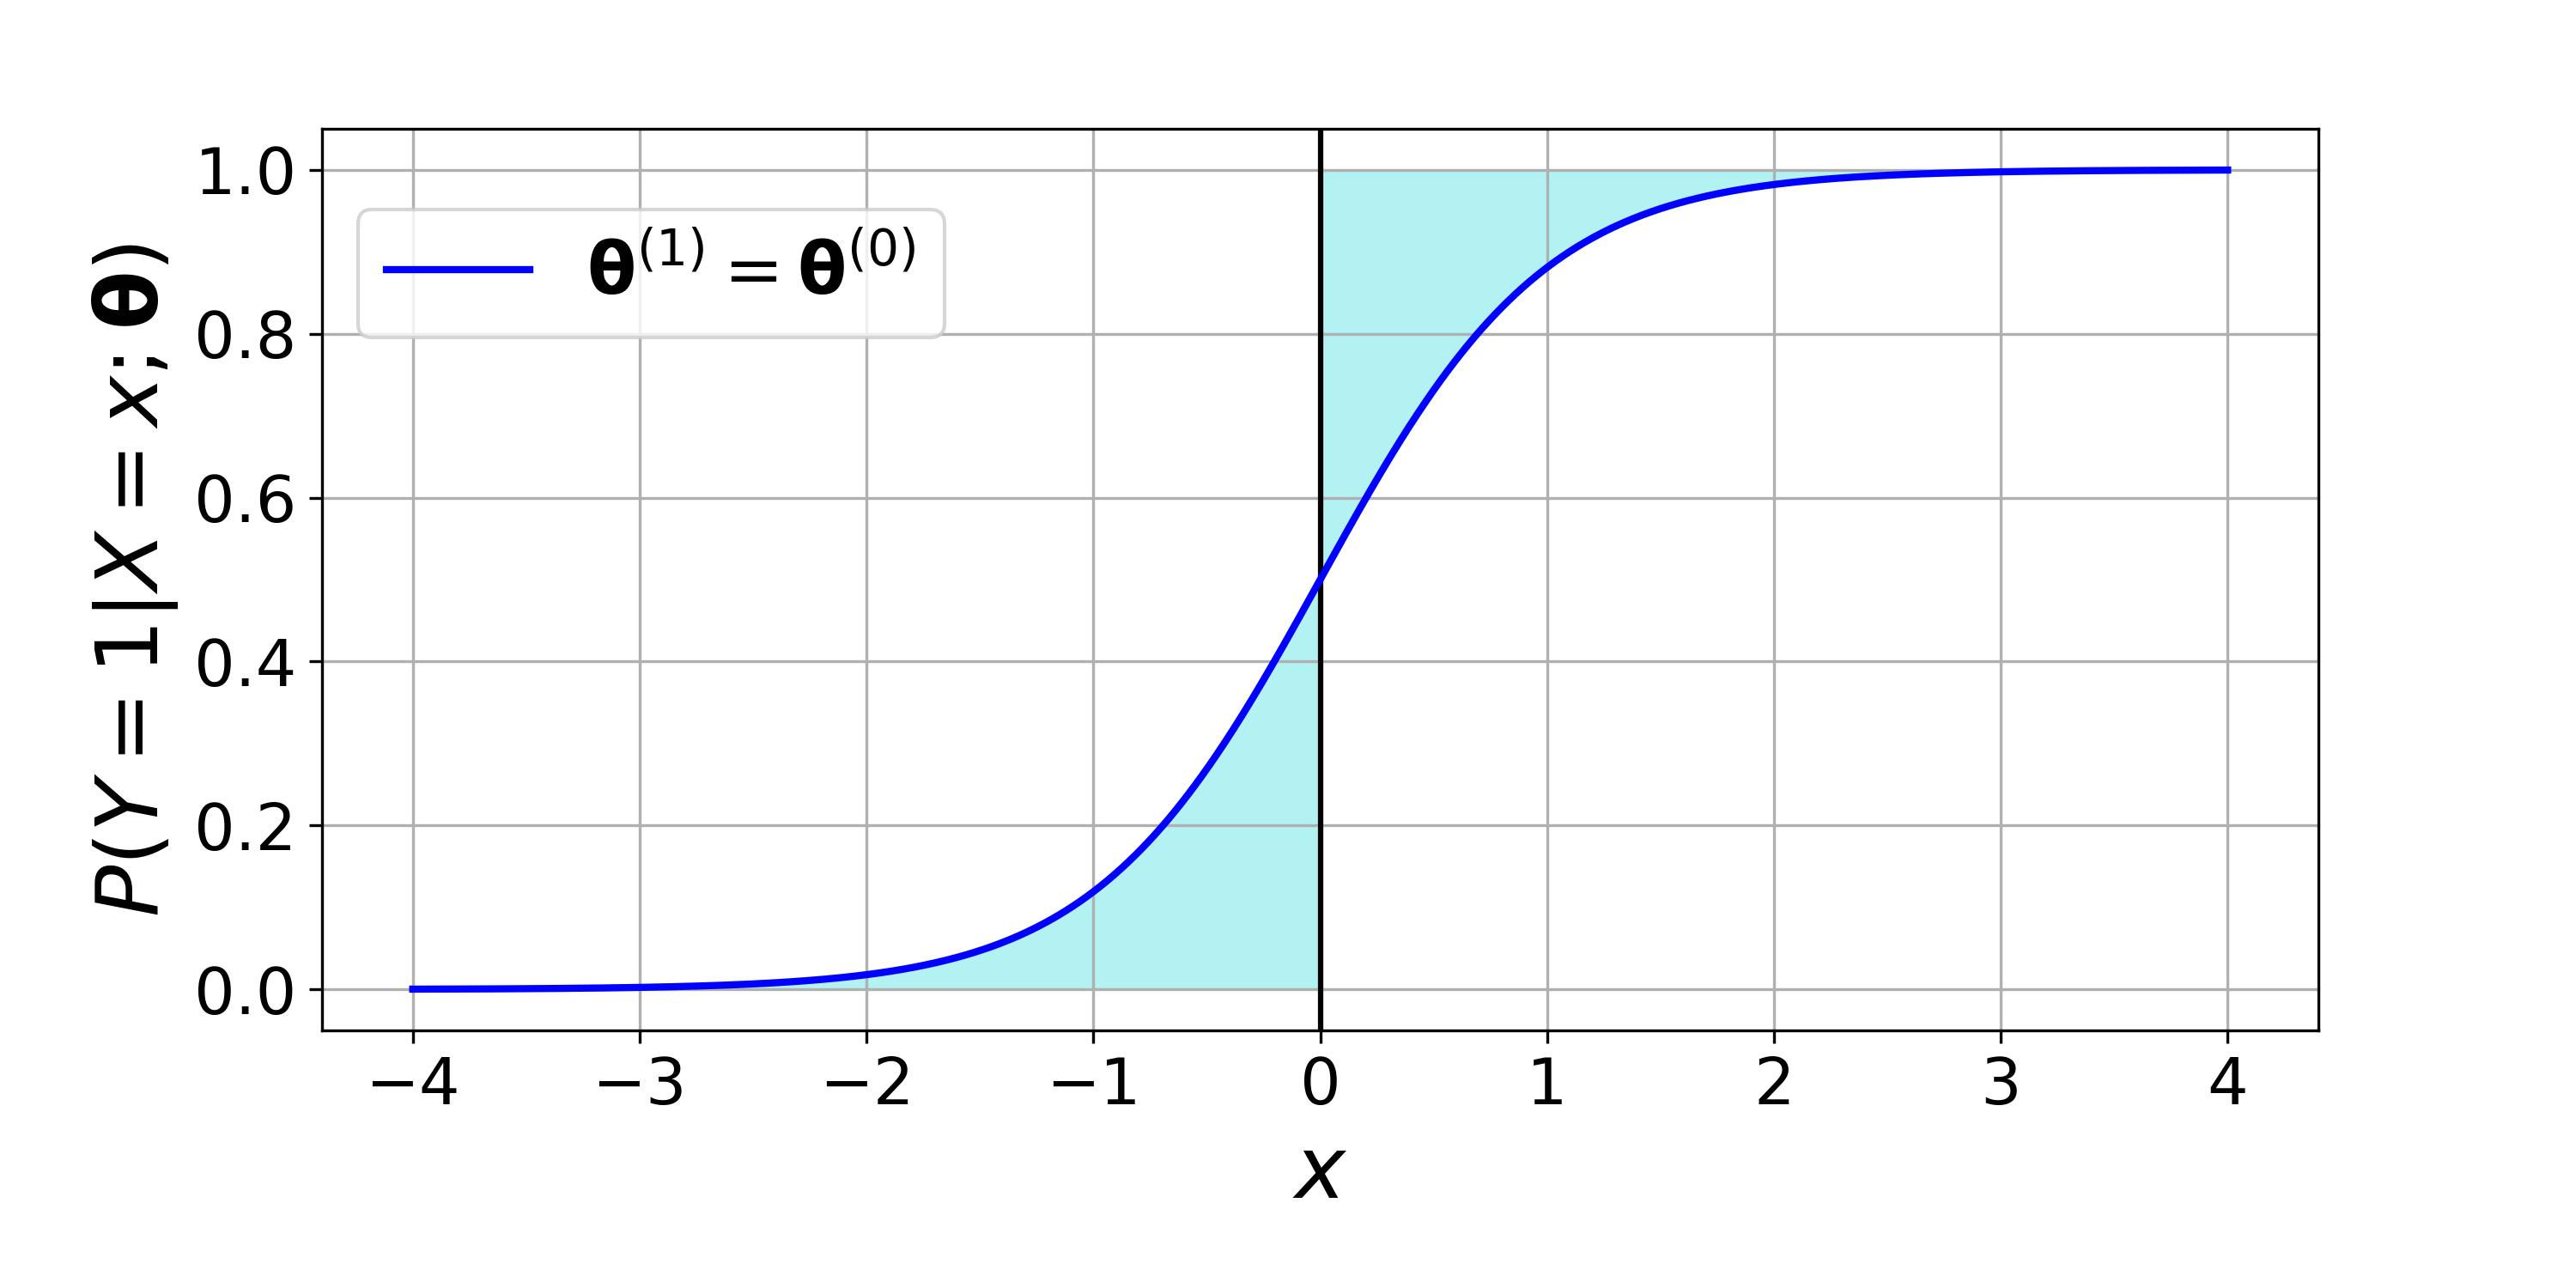
\includegraphics[width=\textwidth, trim=.2in .2in .7in .45in, clip]{./figures_archive/demons_fig/2D_logi_orig.png}
         \captionsetup{width=.95\linewidth}
         \caption{The original model $P(Y|{X};\bm{\theta}^{(0)})$ with the decision boundary that minimizes the expected error rate~($22.2\%$) in Equation~(\ref{eqn_CD:logi_err_rate}).}
         \label{fig_CD:logi_err_rate_unch_a}
  \end{subfigure}
  \begin{subfigure}[t]{0.4\linewidth}
         \centering
         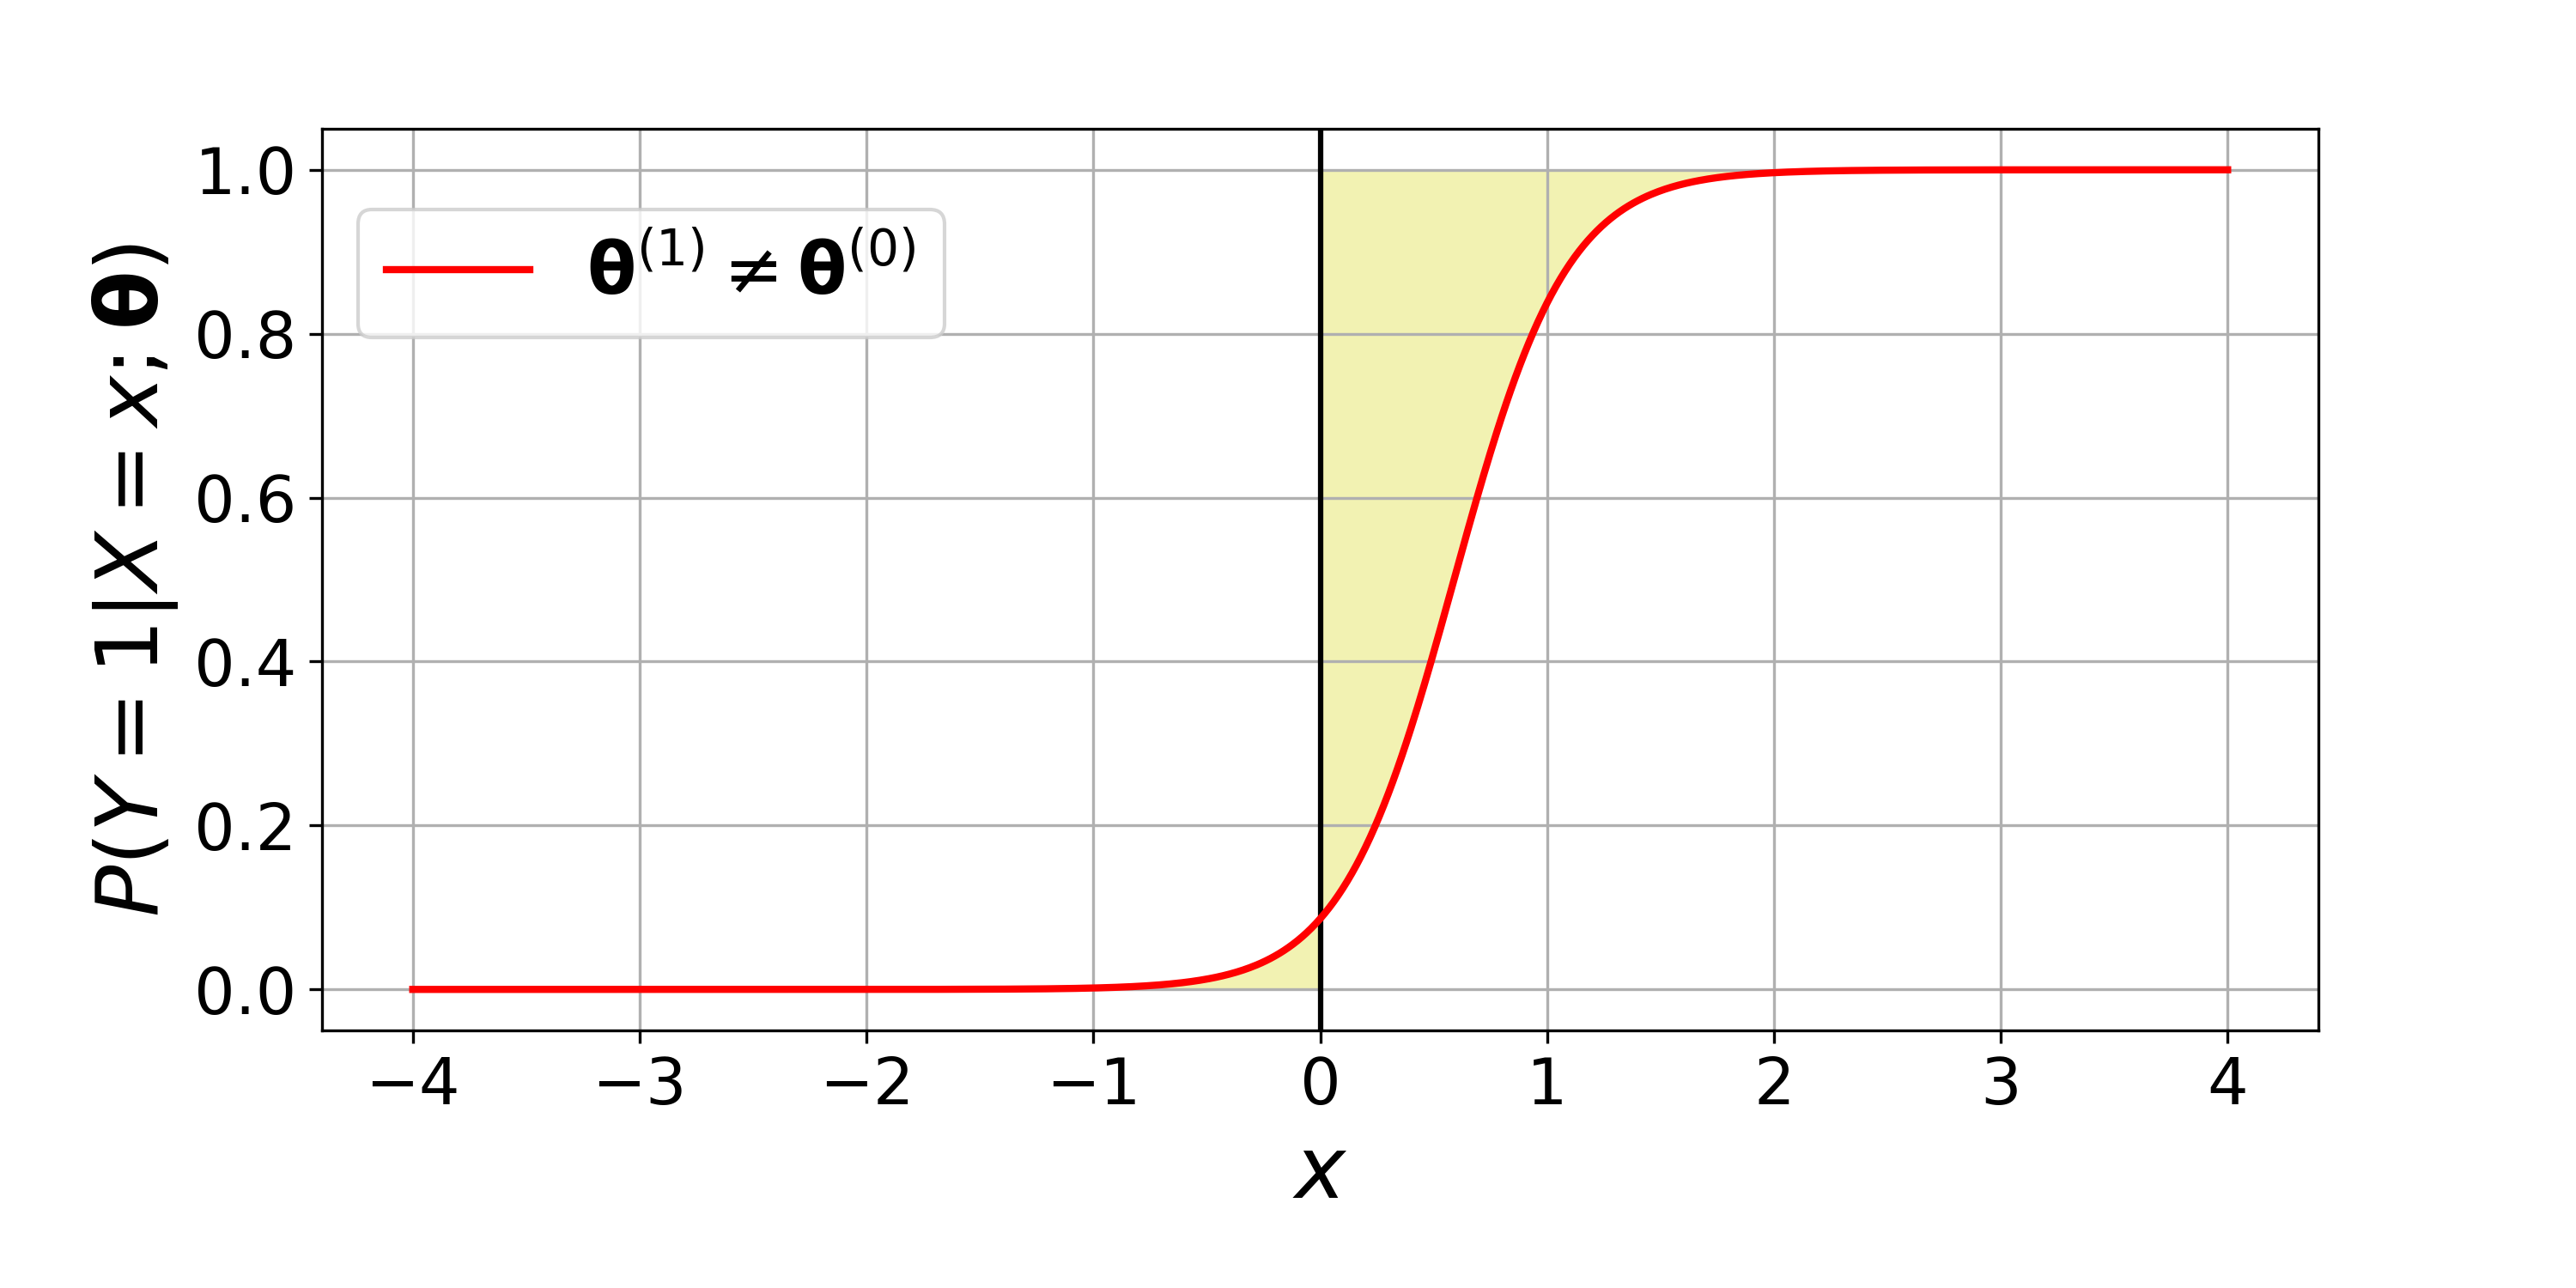
\includegraphics[width=\textwidth, trim=.2in .2in .7in .45in, clip]{./figures_archive/demons_fig/2D_logi_cd.png}
         \captionsetup{width=.95\linewidth}
         \caption{The drifted model $P(Y|{X};\bm{\theta}^{(1)})$ but with unchanged error rate from penal (a).}
         \label{fig_CD:logi_err_rate_unch_b}
  \end{subfigure}

  \begin{subfigure}[t]{0.4\linewidth}
         \centering
	 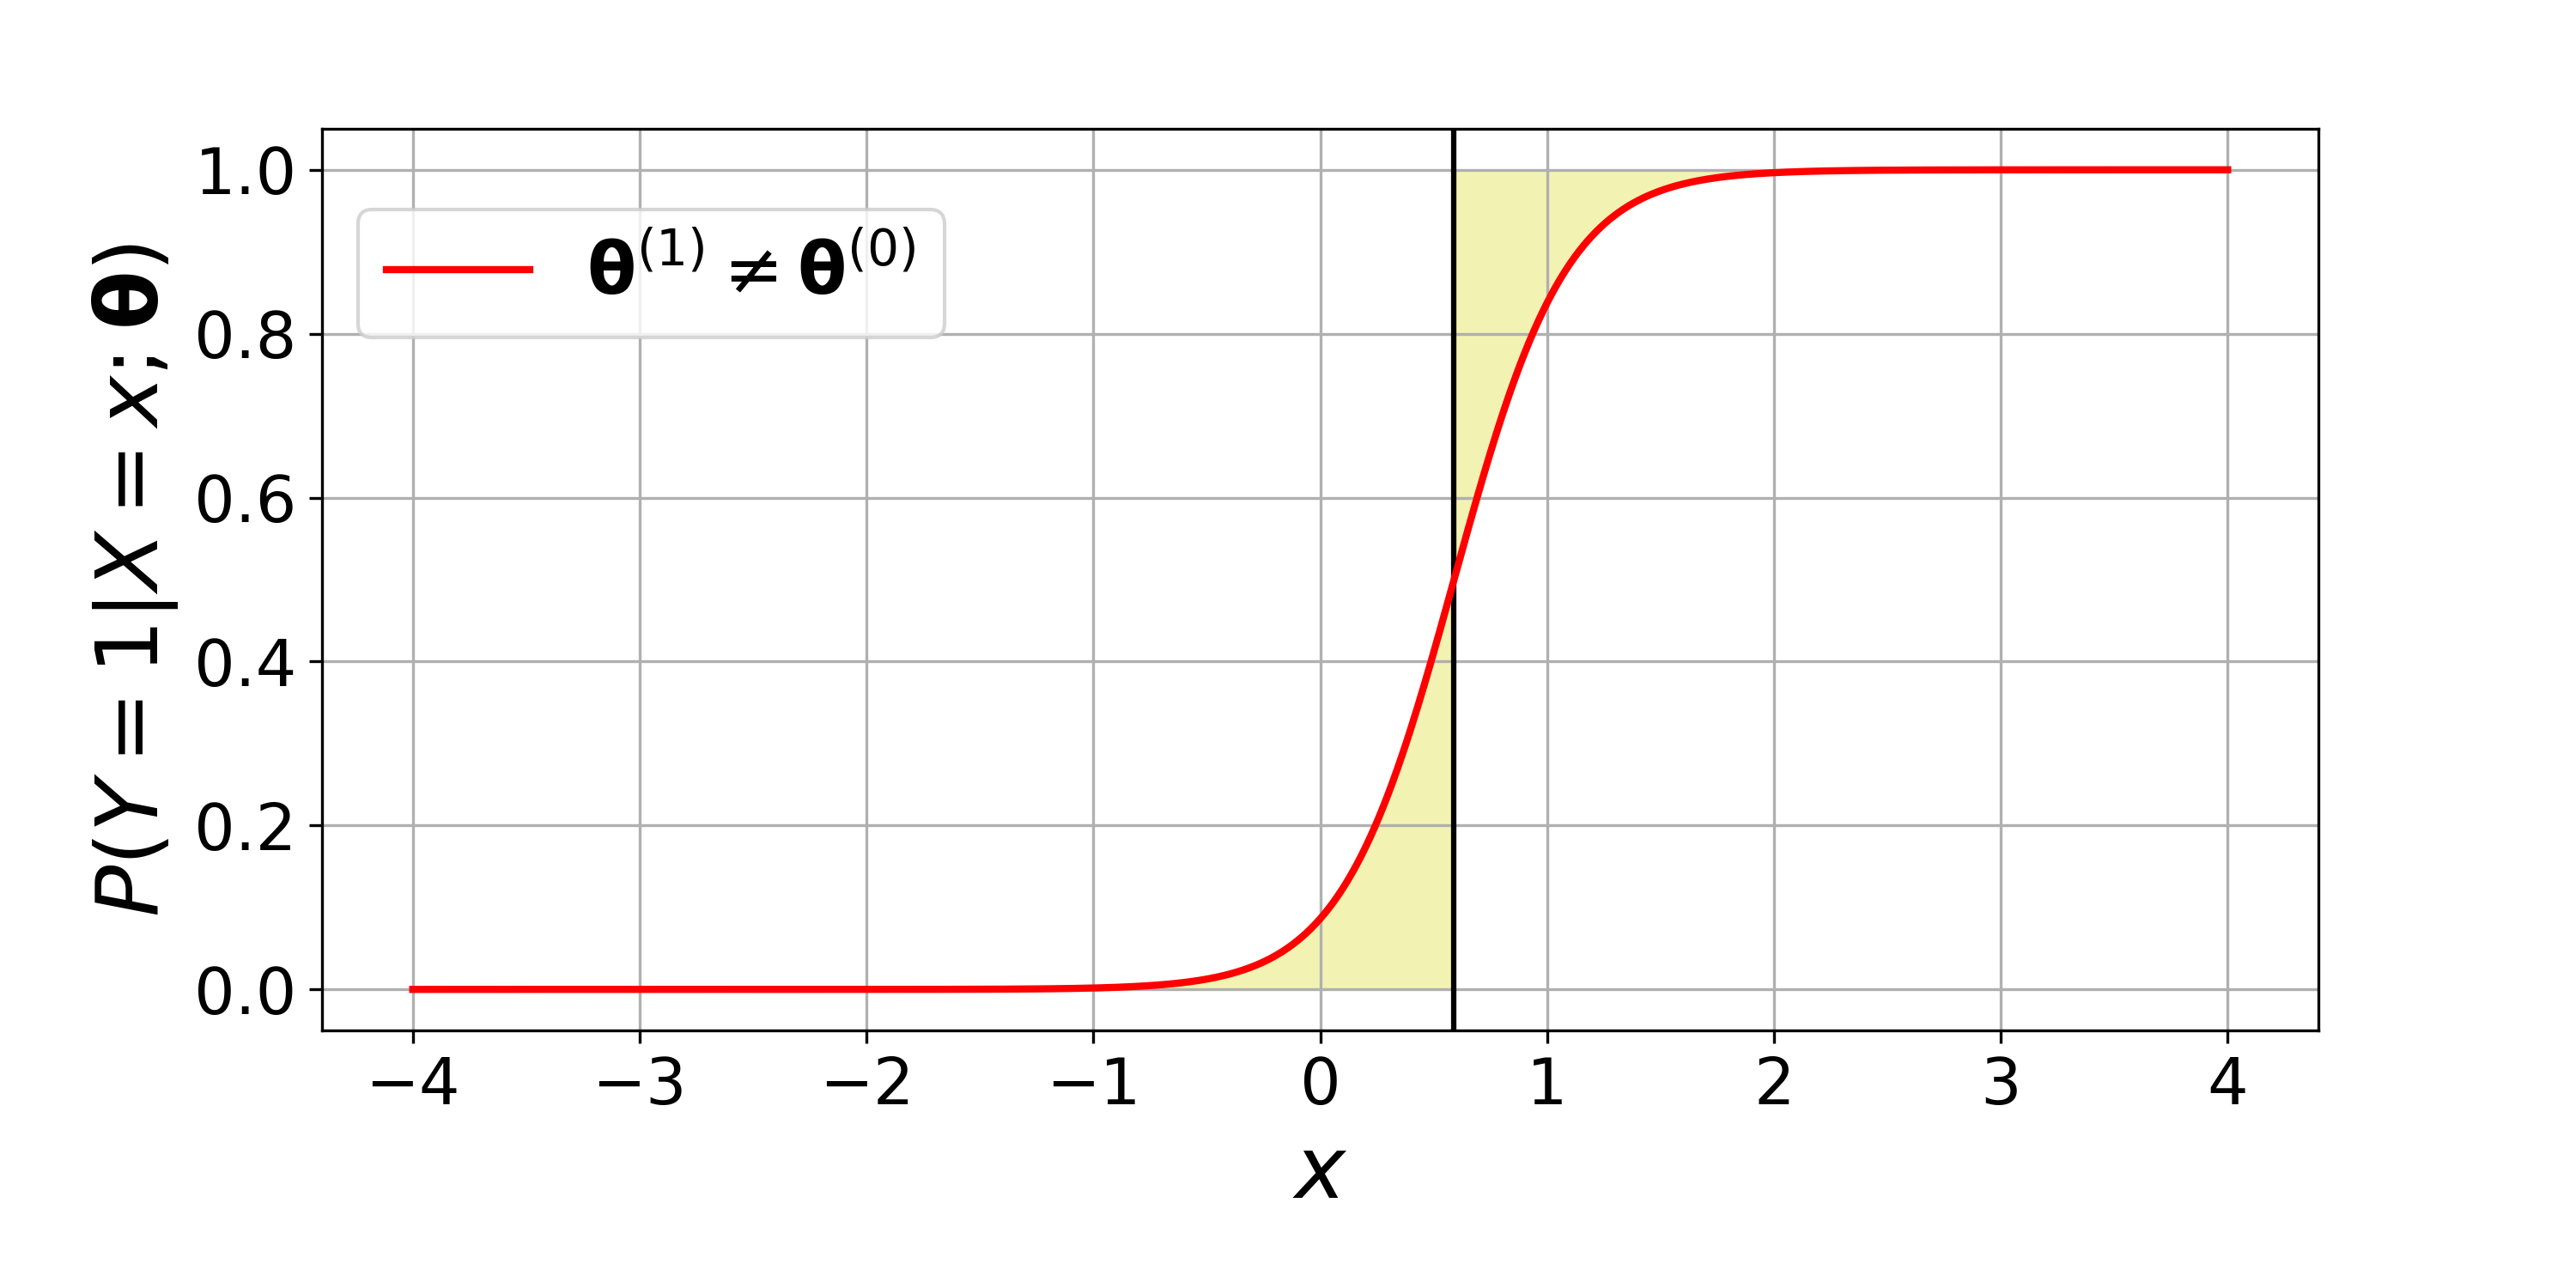
\includegraphics[width=\textwidth, trim=.2in .2in .7in .45in, clip]{./figures_archive/demons_fig/2D_logi_cd_updated.png}
         \captionsetup{width=.95\linewidth}
         \caption{The drifted model $P(Y|{X};\bm{\theta}^{(1)})$ after detecting concept drift and updating the decision boundary to reduce error rate.}
         \label{fig_CD:logi_err_rate_unch_d}
  \end{subfigure}
  \caption{For a simple logistic regression model, demonstration of how concept drift can result in no change in the error rate. The shaded regions are related to the error in Equation~(\ref{eqn_CD:logi_err_rate}).}
  \label{fig_CD:logi_err_rate_unch}
\end{figure}

To further illustrate the above with a more concrete example, consider the following binary simple logistic regression example in which concept drift occurs but with no change in the error rate. The formulas defining the model and the corresponding score vector in this case are
\begin{align}
\begin{aligned}
&P(Y=1|{X};\bm{\theta}) = \frac{\exp\{\bm {X}^{T} \bm {\theta}\}}{1+\exp\{\bm {X}^{T} \bm {\theta}\}}\text{,~and} \\
&\bm {s}(\bm { \theta} ; ( {X}, Y)) = (Y-P(Y=1|{X};\bm{\theta}))\bm {X},
\end{aligned}
\label{eqn_CD:logi_mod_score}
\end{align}
where $\bm{X} = [1, X]^T$ and $\bm{\theta}=[\theta_0, \theta_1]^T$. It is straightforward to verify that the expectation of the score vector is $\bm {0}$, when $\bm{\theta}$ does not change.

Further suppose the $X$ follows a truncated standard normal distribution with density function denoted by $f(x)$~($x\in[-4, 4]$) and the conditional distribution $P(Y|X;\bm{\theta})$ has concept drift with $\bm{\theta}$ changing from $\bm{\theta}^{(0)}$ to $\bm{\theta}^{(1)}$, and define 
\begin{align}
p^{(j)}(X)=P(Y=1|X;\bm{\theta}^{(j)}),~j\in\{0,1\}.
\label{eqn_CD:simp_nota_p}
\end{align}
Figures~\ref{fig_CD:logi_err_rate_unch_a} and~\ref{fig_CD:logi_err_rate_unch_b} plot $p^{(0)}(x)$ and $p^{(1)}(x)$, respectively. Suppose we use the classification rule $\hat{y}(x)=1$ if $p^{(0)}(x)\geq 0.5$ and $\hat{y}(x)=0$ otherwise. Then the conditional and unconditional error rates are

\begin{align}
\begin{aligned}
&P(Y\neq\hat{y}(X)|X;\bm{\theta}^{(j)})
= p^{(j)}(X)(1-\hat{y}(X)) + (1-p^{(j)}(X))\hat{y}(X)\text{,~and} \\
&P(Y\neq\hat{y}(X);\bm{\theta}^{(j)}) = E[P(Y\neq\hat{y}(X)|X;\bm{\theta}^{(j)})] \\ &= \int_{-4}^{4}P(Y\neq\hat{y}(x)|X;\bm{\theta}^{(j)})f(x)dx.
\end{aligned}
\label{eqn_CD:logi_err_rate}
\end{align}
Note that this classifier $\hat{y}(x)$ minimizes the unconditional error rate. As a numerical example, suppose $\bm{\theta} = \bm{\theta}^{(0)}=[0, 2]^T$ so that the true predictive relationship $P(Y=1|{X})$ is as in Figure~\ref{fig_CD:logi_err_rate_unch_a}, the classification rule is $\hat{y}(x)=1$ if $x\geq 0$, and the error rate is $22.2\%$. Now suppose we use the same classifier based on $\bm{\theta}^{(0)}$, but $\bm{\theta}$ changes to $\bm{\theta}^{(1)}=[0.59, 4]^T$ so that the true predictive relationship $P(Y=1|{X})$ is as in Figure~\ref{fig_CD:logi_err_rate_unch_b}. Even though $\bm{\theta}$ has changed, the error rate remains unchanged at $22.2\%$. Clearly, any concept drift detection method based on the error rate will fail to detect the change in $\bm{\theta}$. It is important to note that although the error rate does not change when $\bm{\theta}$ changes from $\bm{\theta}^{(0)}$ to $\bm{\theta}^{(1)}$, the change in $\bm{\theta}$ constitutes an opportunity to improve the classification accuracy if we were to detect the change and update the classification rule based on the new model, i.e., if we were to use the new classifier $\hat{y}(x)=1$ if $x \geq 0.59$~(i.e., if $p^{(1)}(x)\geq 0.5$). This is illustrated in Figure~\ref{fig_CD:logi_err_rate_unch_d}.

In contrast to any error rate monitoring approach, as we have shown earlier under fairly general conditions, the mean of the score vector always changes when $P(Y|\bm{X};\bm{\theta})$ changes. In Section~\ref{ss_CD:cd_no_err_change}, we present a numerical example to further support the analysis here.

\subsection{Interpretations with Empirical Data and Incorrect Models}
\label{ss_CD:sgd_score}
The zero-mean property $E_{\bm{\theta}^{(0)}}[\log{P(Y|\bm{X}; \bm{\theta}^{(0)})}] = \textbf{0}$ of the score vector and the uniqueness of the parameters $\bm{\theta}$ that maximize the expected log-likelihood $E_{\bm{\theta}^{(0)}}[\log P(Y|\bm{X}; \bm{\theta})]$ are guaranteed to hold only when the model is correct; that is, when the supervised learning model $P(Y|\bm{X};\bm{\theta})$ is of the same structure as the true predictive relationship $P(Y|\bm{X})$. Recalling the adage that ``All models are wrong, but some are useful"~(\cite{box1976science})), one might wonder to what extent the results in the previous section are applicable when the structure of the model $P(Y|\bm{X};\bm{\theta})$ differs from the true $P(Y|\bm{X})$. A related question is what should we take to be the empirical counterpart to $E_{\bm{\theta}}[\bm{s}(\bm{\theta}^{(0)};(\bm{X},Y) )]$ when $\bm{\theta}^{(0)}$ is replaced by its estimate from a sample of training data, and the expectation is replaced by a sample average over a set of new data or over the same training data. We address both of these issues in this section and also relate the empirical counterpart to SGD for computational reasons. 

Regardless of whether the model structure is correct, in analogy with Equation~(\ref{eqn_CD:score_exp_zero}) we always have
\begin{align}
\begin{aligned}
&\hat{E}_{(0)}[\bm{s}(\hat{\bm{\theta}}^{(0)};(\bm{X}, Y))] \vcentcolon=\frac{1}{n}\sum_{i=1}^{n}\bm{s}(\hat{\bm{\theta}}^{(0)};(\bm{x}_i, y_i))=\bm{0}, \text{where} \\
&\hat{\bm{\theta}}^{(0)} \vcentcolon =  \argmax_{\bm{\theta}}\hat{E}_{(0)}[\log{P(Y|\bm{X}; \bm{\theta})}] \vcentcolon= \argmax_{\bm{\theta}}\frac{1}{n}\sum_{i=1}^n \log{P(y_i|\bm{x}_i;\bm{\theta})},
\end{aligned}
\label{eqn_CD:score_exp_zero_emp}
\end{align}   
the operator $\hat{E}_{(0)}$ denotes a sample average over the training data $\{(\bm{x}_i, y_i)\}_{i=1}^n$, and $\hat{\bm{\theta}}^{(0)}$ is the maximum-likelihood estimator~(MLE) of $\bm{\theta}^{(0)}$ for the training data. That is, when we fit a model using MLE, the gradient of the training log-likelihood is identically zero, i.e., $\nabla_{\bm{\theta}}\hat{E}_{(0)}[\log{P(Y|\bm{X}; {\bm{\theta}})}]|_{\bm{\theta}=\hat{\bm{\theta}}^{(0)}} \vcentcolon=\nabla_{\bm{\theta}}\frac{1}{n}\sum_{i=1}^n \log{P(y_i|\bm{x}_i;{\bm{\theta}})|_{\bm{\theta}=\hat{\bm{\theta}}^{(0)}}}=\frac{1}{n}\sum_{i=1}^n\bm{s}(\hat{\bm{\theta}}^{(0)};(\bm{x}_i, y_i)) = \hat{E}_{(0)}[\bm{s}(\hat{\bm{\theta}}^{(0)};(\bm{X}, Y))]=\bm{0}$, even if the model is not the correct structure. Thus, (\ref{eqn_CD:score_exp_zero_emp}) is the empirical counterpart of (\ref{eqn_CD:score_exp_zero}) with the estimated $\hat{\bm{\theta}}^{(0)}$ taking the place of the true $\bm{\theta}^{(0)}$. 

Now suppose the true predictive relationship $\tilde{P}(\tilde{Y}|\tilde{\bm{X}})$ changes from $P(Y|\bm{X})$ over some new set of data $\{(\tilde{\bm{x}}_i, \tilde{y}_i)\}_{i=1}^{\tilde{n}}$. In this case a different set of parameters $\hat{\bm{\theta}}^{(1)} \neq \hat{\bm{\theta}}^{(0)}$ for the same supervised learning model structure $P(Y|\bm{X};\bm{\theta})$ will generally provide a better fit to the new data than did $\hat{\bm{\theta}}^{(0)}$, where 
\begin{align}
\begin{aligned}
\hat{\bm{\theta}}^{(1)} \vcentcolon= \argmax_{\bm{\theta}}\hat{E}_{(1)}[\log{P(\tilde{Y}|\tilde{\bm{X}}; \bm{\theta})}] \vcentcolon= \argmax_{\bm{\theta}}\frac{1}{\tilde{n}}\sum_{i=1}^{\tilde{n}} \log{P(\tilde{y}_i|\tilde{\bm{x}}_i;\bm{\theta})},
\end{aligned}
\label{eqn_CD:score_exp_nonzero_emp}
\end{align}   
and the operator $\hat{E}_{(1)}$ denotes the sample average over the new data. Thus, the gradient $\nabla_{\bm{\theta}}\hat{E}_{(1)}[\log{P(\tilde{Y} | \tilde{\bm{X}}; {\bm{\theta}})}]|_{\bm{\theta}=\hat{\bm{\theta}}^{(0)}} \vcentcolon= \nabla_{\bm{\theta}}\frac{1}{\tilde{n}}\sum_{i=1}^{\tilde{n}} \log{P(\tilde{y}_i | \tilde{\bm{x}}_i; {\bm{\theta}})}|_{\bm{\theta}=\hat{\bm{\theta}}^{(0)}} = \frac{1}{\tilde{n}} \sum_{i=1}^{\tilde{n}} \bm{s}(\hat{\bm{\theta}}^{(0)};(\tilde{\bm{x}}_i, \tilde{y}_i)) = \hat{E}_{(1)}[\bm{s}(\hat{\bm{\theta}}^{(0)};(\tilde{\bm{X}}, \tilde{Y}))]$ of the log-likelihood for the new data~(but with the gradient evaluated at the original estimate $\hat{\bm{\theta}}^{(0)}$) will generally differ from zero. The more $\tilde{P}(\tilde{Y}|\tilde{\bm{X}})$ changes from $P(Y|\bm{X})$, the more we expect $\hat{\bm{\theta}}^{(1)}$ to differ from $\hat{\bm{\theta}}^{(0)}$, and the more we expect the new average score vector $\hat{E}_{(1)}[\bm{s}(\hat{\bm{\theta}}^{(0)};(\tilde{\bm{X}}, \tilde{Y}))]$ to differ from $\bm{0}$. This provides the justification for our score-based concept drift monitoring approach, which tracks the mean of the score vector $\bm{s}(\hat{\bm{\theta}}^{(0)};(\bm{X}_i, Y_i)) = \nabla_{\bm{\theta}}\log P(Y_i|\bm{X}_i; \bm{\theta})|_{\bm{\theta}=\hat{\bm{\theta}}^{(0)}}$ to detect and analyze changes in it. 

If the supervised learning model $P(Y|\bm{X};\bm{\theta})$ is of the same structure as the true predictive relationship $P(Y|\bm{X})$, both $P(Y|\bm{X})$ and $P(\bm{X})$ are constant across the training data $\{(\bm{x}_i, y_i)\}_{i=1}^n$, and $n \to \infty$, then under some regularity conditions the MLE $\hat{\bm { \theta}} ^{ (0)}$ is consistent and  $\hat{E}_{(0)} [\bm{s}(\hat{\bm { \theta}} ^{ (0)};(\bm {X}, Y))] \to E_{\bm { \theta} ^{ (0)}}[\bm{s}(\hat{\bm { \theta}} ^{ (0)};(\bm {X}, Y))] \to E_{\bm { \theta} ^{ (0)}}[\bm{s}(\bm { \theta} ^{ (0)};(\bm {X}, Y))] = \bm {0}$. In this case, there is no distinction between the theoretical version of the score-based monitoring arguments and their empirical version discussed above. With large $n$, SGD is often used to fit models to the training data, which involves approximating the gradient of the log-likelihood function using individual training observations or mini-batches of training observations at each iteration of the optimization algorithm. The SGD estimator of $\bm { \theta} ^{ (0)}$ converges to the batch MLE under certain conditions involving step size and other considerations~(see, e.g., Theorem 4.7 of \cite{bottou2018optimization}). In this case, under the same asymptotic conditions stated above, the SGD estimator $\hat {\bm { \theta}}_{\mathrm{SGD}}$ is also consistent and $\hat{E}_{(0)} [\bm{s}(\hat{\bm { \theta}}_{\mathrm{SGD}};(\bm {X}, Y))] \to \bm{0}$ as $n \to \infty$. 

The score-based approach does not add much extra cost to the current framework of training and using models. For retrospective analysis, the sample score vectors are a byproduct of the SGD~(or related optimizers, e.g., ADAM~(\cite{kingma2014adam})), since the mini-batch gradients are of the form $\nabla _{\bm { \theta}} \sum _{i=1} ^{m} \log{P(y_i|\bm {x}_i;\bm{\theta})} = \sum _{i=1} ^{m} \bm{s}(\bm { \theta};(\bm {x}_i, y_i))$, where $m$ is the batch size. Even for prospective analysis, prediction of new data usually partially calculates the score vectors. For example, prediction for neural networks requires forward-propagation, and another backward-propagation in memory would generate the score vector. Thus, we do not need much extra computation to apply the score-based approach.

With finite training data size $n$ and finite new sample sizes $\tilde{n}$ for monitoring~(including $\tilde{n}=1$), noise in $\bm{s}(\bm { \theta};(\bm {x}_i, y_i))$ and its sample averages must be considered. In particular, we need to distinguish by how much $\bm{s}(\hat{\bm { \theta}}^{(0)};(\bm {x}_i, y_i))$~(or its sample average over some moving time window) should differ from $\bm{0}$ before we conclude that $P(Y|\bm{X})$ has changed. The MEWMA monitoring strategy in the next section is designed to distinguish this type of noise from legitimate changes in $P(Y|\bm{X})$. Moreover, for models fitted with regularization, the gradient of the log-likelihood itself is not zero over the training data, because the regularization penalty is included in the optimization objective function. Regardless, the score-based monitoring method can still be applied with the minor modification to the score vectors discussed in Section~\ref{ss_CD:high_dim_score}.

\subsection{An MEWMA Approach for Monitoring the Score Vector}
\label{ss_CD:MEWMA}
As discussed in the previous sections, monitoring for concept drift reduces to monitoring for changes over time in the mean of the score vector. Among other challenges, this requires distinguishing between noise in the score vectors for individual observations vs. an actual mean change. Monitoring for changes in the mean of random vectors~(e.g., a set of multivariate quality-related measures) while distinguishing from noise is an old and well-researched problem in the SPC literature. The MEWMA has emerged as one of the most effective techniques for this, and in this section we develop it for monitoring the score vector mean vector.

The MEWMA at time $t$, denoted by $\bm{z}_t$, is defined recursively~(for $t=1,2,\cdots$) via:
\begin{align}
\bm {z}_t = \lambda \bm {s}_t + (1 - \lambda) \bm {z} _{t-1},
\label{eqn_CD:ewma}
\end{align}
where $\bm {s}_t$ is the to-be-monitored random vector at time $t$, which in our case is the score vector $\bm {s}_t \vcentcolon= \bm{s}(\hat{\bm { \theta}}^{(0)};(\bm {x}_t, y_t))$; $ \lambda$ is a weighting parameter; and $\bm{z}_0$ can be initialized as the sample mean of $\bm {s}_t$ over some small initial batch of observations. An equivalent expression for the recursive relationship~(\ref{eqn_CD:ewma}) is $\bm {z}_t = \lambda\sum _{\tau=1}^t (1-\lambda) ^{t-\tau} \bm{s} _{\tau} + (1-\lambda)^t \bm{z}_0$, which gives exponentially decaying weights to the historic observations up to $\bm{s}_t$. Smaller $\lambda$ in the MEWMA formula corresponds to more slowly decaying weights and thus longer effective windows over which the exponentially-weighted averages are computed. The effective window length is sometimes viewed as $\sum _{j=0}^\infty (1-\lambda)^j = \frac{1}{\lambda}$. The choice of $\lambda$ should depend on the application of interest, with the following trade-off. Smaller $\lambda$ translates to a larger effective window length, which gives a lower-variance estimate of the mean of $\bm{s}_t$ by smoothing out more noise~(which generally results in better detection of small changes), but it also makes the MEWMA more sluggish~(which results in longer delays in detecting large changes). If there is no need to detect changes in $P(Y|\bm{X})$ in fewer than some number~(say $D$) of observations, then there is no need to have the effective window length $\frac{1}{\lambda}$ smaller than $D$, in which case one should  select $\lambda \leq \frac{1}{D}$.

Since $\bm{s}_t$ and $\bm{z}_t$ are vectors, and we desire to detect changes in the mean of $\bm{s}_t$ in any direction, our MEWMA approach monitors the Hotelling $T^2$ statistic 
\begin{align}
T_t^2 = (\bm {z}_t-\bar { \bm {s}})^T \widehat {\bm { \Sigma}} ^{-1}(\bm {z}_t-\bar { \bm {s}}),
\label{eqn_CD:hotellingt2}
\end{align}
where $\widehat {\bm { \Sigma}}$ and $\bar {\bm{s}}$ are the covariance matrix and sample mean vector of $\bm {s}_t$, respectively, estimated from the training and Phase-I data, as described in Figure~\ref{fig_CD:proc_mon_score_monitoring} and later parts of this section. If $T_t^2$ at some $t$ exceeds a specified upper control limit~($UCL$) determined as described later, this is taken to be an indication that $P(Y|\bm{X})$ in the time-vicinity of observation $t$ has changed from what it was when $\hat{\bm{\theta}}^{(0)}$ was estimated. The convention that we recommend and that we have used in all of our later examples in the paper is to estimate $\bar {\bm{s}}$ from only the Phase-I data and $\widehat {\bm { \Sigma}}$ from only the training data. The reason we do not use any Phase-I data to estimate $\widehat {\bm { \Sigma}}$ is that the control limits are determined from the Phase-I data, and estimating $\widehat {\bm { \Sigma}}$ from the same Phase-I data can result in a form of overfitting and a UCL that is too small, which results in too many false alarms. The reason we not use any training data to estimate $\bar {\bm{s}}$ is that if there is concept drift between the training and Phase-I data and we use the training data to estimate $\bar { \bm {s}}$, then $\bm {z}_t-\bar { \bm {s}}$ will not be zero-mean over the Phase-I data, which can result in a UCL that is too large, which reduces the sensitivity to concept drift in Phase-II. Note that if there is concept drift between the training and Phase-I data, this can be detected via our retrospective analysis, as illustrated in the later examples. 


\begin{figure}[!htbp]
\centering
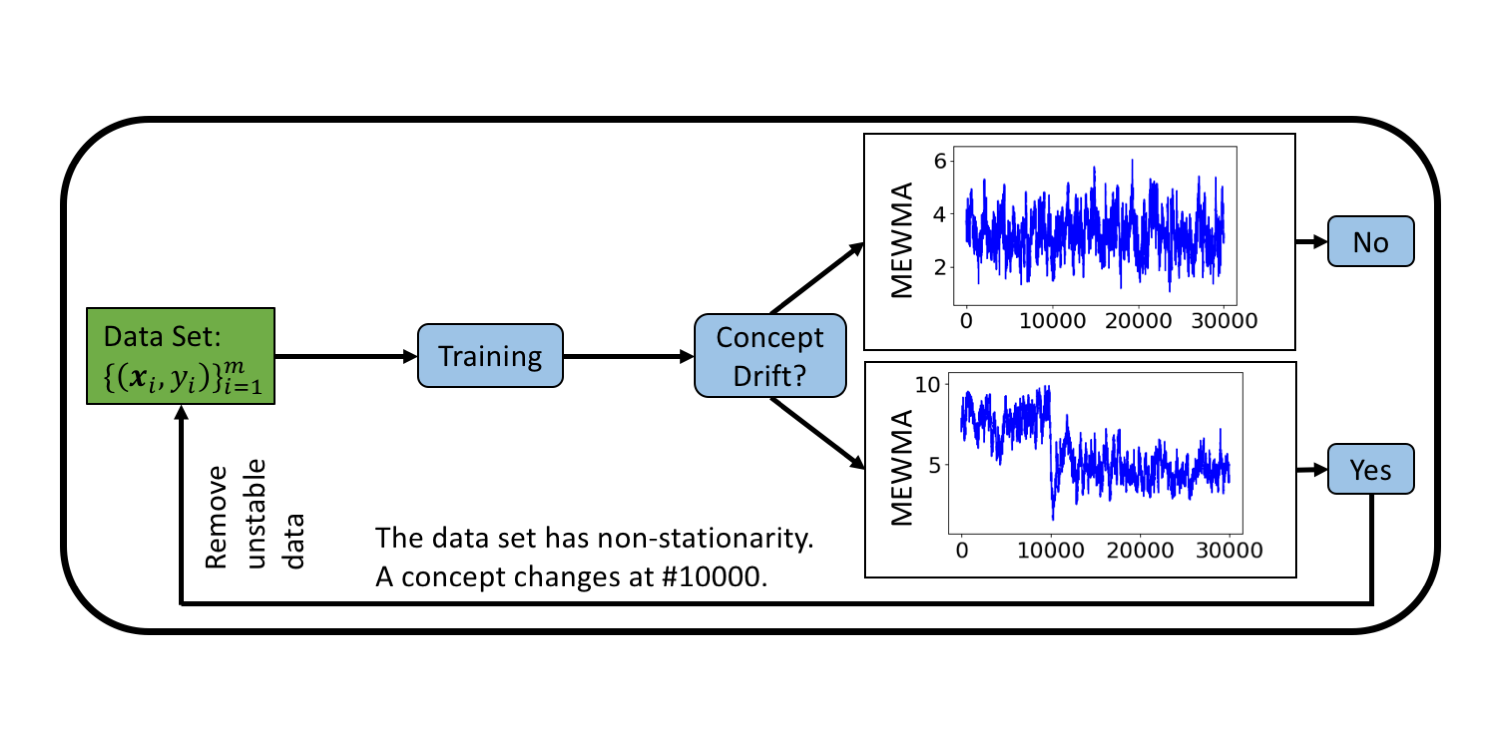
\includegraphics[width = .8\linewidth, trim=.35in .68in .35in .69in, clip]{./figures_archive/flow_chart/Retrospective_2.png}
\caption{Step $1$ of the score-based concept drift framework. A retrospective analysis to determine whether the training data to which the model is fitted are stable~(as in the top plot) vs. whether concept drift occurred over the training data~(as in the bottom plot).}
  \label{fig_CD:proc_mon_score_retro}
\end{figure}

\begin{figure}
\centering
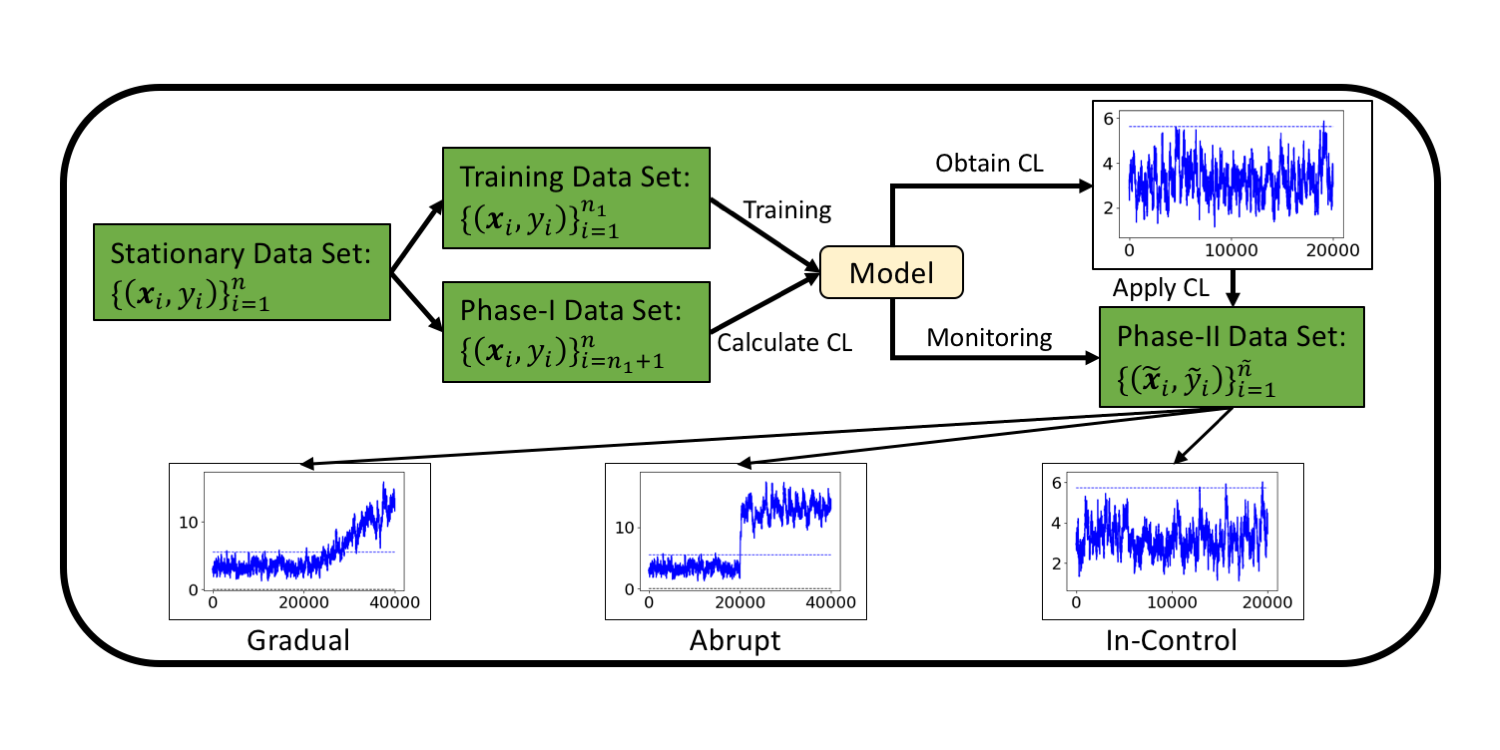
\includegraphics[width = .8\linewidth, trim=.35in .48in .35in .49in, clip]{./figures_archive/flow_chart/Monitoring_2.png}
\caption{Step $2$ of the score-based concept drift framework. A retrospective analysis first splits the stationary data from Step $1$ into a training set~(to which the model is fitted) and a Phase-I set~(which is used to establish the control limit for Phase-II). Then a prospective Phase-II analysis is used to monitor new data for concept drift as each new $(\bm{X}, Y)$ observation is collected.}
\label{fig_CD:proc_mon_score_monitoring}
\end{figure}

\begin{figure}
\centering
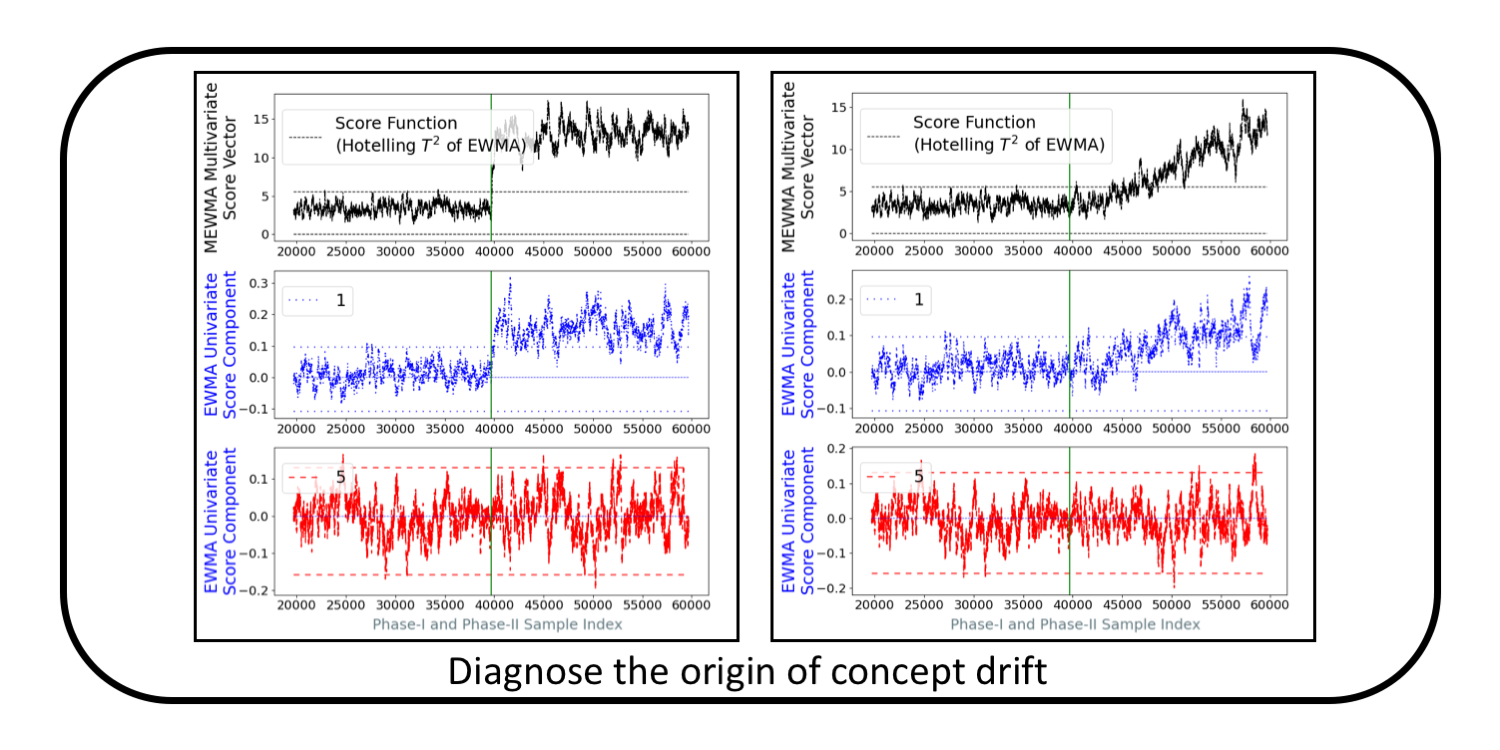
\includegraphics[width = .8\linewidth, trim=.35in .21in .35in .21in, clip]{./figures_archive/flow_chart/Diagnose_2.png}
\caption{Step $3$ of the score-based concept drift approach. A diagnostic analysis to help identify the nature of the concept drift once it is detected in either the retrospective stage in Step $1$ or the Phase-II monitoring stage in Step $2$. The left and right plots depict two different types of concept drift -- an abrupt change~(the left plots) and a gradual change~(the right plots). The legend numbers are indices of covariates in our models.}
\label{fig_CD:proc_mon_score_diagnosis}
\end{figure}

The score-based concept drift monitoring framework is broken into three steps and depicted in Figures~\ref{fig_CD:proc_mon_score_retro},~\ref{fig_CD:proc_mon_score_monitoring}, and~\ref{fig_CD:proc_mon_score_diagnosis} for Steps $1$, $2$, and $3$, respectively. The three steps will be illustrated in more detail in the later examples. In Step 1, we collect a batch of data in time order, $\{\bm {x}_i, y_i\} _{i=1} ^{m}$, where $m$ denotes the sample size of this batch. Then, after fitting a preliminary supervised learning model to these data, a retrospective analysis is conducted by applying the MEWMA to these same data. If the MEWMA indicates these data are stable and no significant concept drift is detected~(as in the top plot in Figure~\ref{fig_CD:proc_mon_score_retro}), we proceed to Step $2$. On the other hand, if the MEWMA detects significant concept drift in these data (as in the bottom plot in Figure~\ref{fig_CD:proc_mon_score_retro}, where the first third of the data appears to differ from the latter two-thirds) then one can discard a portion of the data prior to the concept drift in attempt to ensure that the remaining data are stable. For other kinds of concept drift, like gradual drifting or seasonality as in the later bike-sharing example in Section~\ref{ss_CD:bs_ds}, we can try to modify the model by incorporating other covariates to reduce the concept drift. This retrospective analysis would then be repeated~(perhaps multiple times) on the remaining data to verify whether it was stable vs. experienced concept drift. When the remaining data are deemed stable, then we proceed to Step $2$, which is depicted in Figure~\ref{fig_CD:proc_mon_score_monitoring}.

Let $n\leq m$ denote the size of the stable data from Step $1$ and denote these data by $\mathcal{D} \vcentcolon=\{\bm {x}_i, y_i\} _{i=1} ^{n}$. The purpose of Step $2$ is to establish the $UCL$  and then to prospectively monitor new data for concept drift, as the new data are collected. To establish the $UCL$, we divide $\mathcal{D}$ into two parts: $ \mathcal{D}_1 \vcentcolon= \{\bm {x}_i, y_i\} _{i=1} ^{n_1}$ and $\mathcal{D}_2 \vcentcolon= \{\bm {x}_i, y_i\} _{i=n_1+1} ^{n}$. The first part, $\mathcal{D}_1$, is used to retrain the parametric supervised learning model of interest, and the second part, $\mathcal{D}_2$, is used to establish the $UCL$ in what is commonly referred to as a Phase-I analysis in the SPC literature. In the Phase-I analysis, the score vectors for the $\mathcal{D}_2$ data are computed, based on the model fitted to the $\mathcal{D}_1$ data. The MEWMA statistics $\{\bm{z}_t\}_{t=n_1+1}^n$ and $T^2$ statistics $\{T_t^2\}_{t=n_1+1}^n$ are then computed for the $\mathcal{D}_2$ data. The user specifies a desired false alarm probability $\alpha$~(e.g., $\alpha=0.0001$, $\alpha=0.001$, etc.), and the $UCL$ is set as the $1-\alpha$ sample quantile of $\{T_t^2\}_{t=n_1+1}^n$. After computing the $UCL$ in Phase-I, in Phase-II the MEWMA with this $UCL$ is applied prospectively to the sample score vectors for a new set of ``on-line" data $\tilde{\mathcal{D}}\vcentcolon=\{\tilde{\bm{x}}_i,\tilde{y}_i\}_{i = 1}^{\tilde{n}}$~(i.e., new data for which the fitted supervised learning model is to be used to predict the response, e.g., new credit card applicants who are being scored for credit risk by the fitted model). The purpose of the Phase-II analysis is to detect as quickly as possible if concept drift occurs in the new data, so that the supervised learning model can be updated accordingly. 

The purpose of Step $3$, depicted in Figure~\ref{fig_CD:proc_mon_score_diagnosis}, is to conduct a diagnostic analysis to help determine the nature of the concept drift, if any drift is detected in Phase-II. This involves plotting the $T_t^2$ statistic v.s. $t$ over the data set of interest, which is depicted in the top plots in Figure~\ref{fig_CD:proc_mon_score_diagnosis}. Note that the $T^2$ statistic aggregates changes in any of the components of the score vector into a single scalar statistic. To provide richer diagnostic information and help understand which parameters have changed, analogous univariate EWMA control charts for~(transformed) individual components of the score vector should also be constructed, which is depicted in the bottom plots in Figure~\ref{fig_CD:proc_mon_score_diagnosis}. We describe these univariate control charts in Section~\ref{s_CD:decou_cd}.

The Step $3$ diagnostic procedure can also be used in a purely retrospective analysis following Step $1$, if it is desired to understand the nature of the nonstationarity in $P(Y|\bm{X};\bm{\theta})$ over any set of training data to which a supervised learning model is fitted.

For the other methods based on scalar metrics~(e.g., error rates) to which we compare our approach and for the transformed components of the score vector that we describe in Section~\ref{s_CD:decou_cd}, we use univariate EWMA~(\cite{roberts1959control}) control charts because the EWMA in Equation~(\ref{eqn_CD:ewma}) is a scalar in this case. One main difference between a univariate EWMA and an MEWMA is that the MEWMA $T^2$ statistic aggregates the changes in the mean vector into a single scalar statistic, and only larger values of $T^2$ indicate a change in the mean from $\bar{\bm{s}}$. Thus only an $UCL$ is needed in the MEWMA. In contrast, the univariate version of the EWMA in Equation~(\ref{eqn_CD:ewma}) to detect changes in the mean of a scalar random variable are two-sided in nature and have a lower control limit~($LCL$) as well as a $UCL$. Changes in the mean are indicated by the univariate EWMA statistic falling either below the $LCL$ or above the $UCL$.


\subsection{Handling High-Dimensional and Regularized Models}
\label{ss_CD:high_dim_score}
Many machine learning models are becoming increasingly complex, and some state-of-the-art models can have millions of parameters, e.g., deep neural networks. With such high-dimensional parameters, the sample covariance matrix $\widehat {\bm { \Sigma}}$ in Equation~(\ref{eqn_CD:hotellingt2}), which must be inverted, is very likely to be singular or close to it. For example, when the sample size of our training data~(denoted by $n_1$ as in Section~\ref{ss_CD:MEWMA}) is smaller than the number of parameters, the sample covariance is always singular. 

The preceding solution would be model specific in that the chosen subset of parameters would depend on the structure of the model. A more general solution is to modify the covariance matrix to circumvent the problem of inverting a singular or poorly-conditioned matrix. One way to accomplish this is to add a nugget parameter~(borrowing terminology from Gaussian process modeling) to all diagonal entries of $\widehat {\bm { \Sigma}}$. Specifically, for some $\delta>0$, we substitute $\widetilde {\bm { \Sigma}} \vcentcolon= \widehat {\bm { \Sigma}}+ \delta \mathbf {I}$ for $\widehat {\bm { \Sigma}}$ in Equation~(\ref{eqn_CD:hotellingt2}). To understand the effect of this nugget parameter, denote the eigen-decomposition of the sample covariance matrix as $\widehat {\bm { \Sigma}} = \mathbf {Q}\bm { \Lambda} \mathbf {Q}^T$, where $\mathbf {Q}$ is an orthogonal matrix of eigenvectors and $\bm{\Lambda}=diag\{\lambda_1, \lambda_2,\cdots, \lambda_{q}\}$, (where $q=dim(\bm{\theta})$), is a diagonal matrix of eigenvalues, and suppose the eigenvalues are arranged in non-increasing order. Then, we can write the approximated sample covariance matrix as $\widetilde {\bm { \Sigma}} = \mathbf {Q}\widetilde{\bm { \Lambda}} \mathbf {Q}^T$, where $\widetilde{\bm { \Lambda}} \vcentcolon= \bm { \Lambda} + \delta \mathbf {I}$. Using $\widetilde {\bm { \Sigma}}$ in place of $\widehat {\bm { \Sigma}}$ in Equation~(\ref{eqn_CD:hotellingt2}) suppresses unimportant directions of variation. The resulting MEWMA with this modified covariance matrix would not have the issue of ill-conditioning. 

Another way to accomplish this is to use a pseudo-inverse of $\widehat {\bm { \Sigma}}$ in Equation~(\ref{eqn_CD:hotellingt2}) instead of its actual inverse, after dropping any eigenvalues $\lambda_i$ with $\lambda_1/\lambda_i>\gamma$ for some specified maximum condition number $\gamma$. Define the diagonal matrix $\bm { \Lambda} ^{-}=diag\{\lambda_1^{-1},\lambda_2^{-1},\cdots,\lambda_k^{-1},0,\\ \cdots,0\}$ where $\lambda_k$ is the smallest eigenvalue with $\lambda_1/\lambda_k$ no greater than $\gamma$. Then, the pseudo-inverse is defined as $\widehat {\bm { \Sigma}} ^{-} = \mathbf {Q}\bm { \Lambda}^{-}\mathbf {Q}^T$. This is equivalent to applying principal component analysis to $\bm{s}_t$ and retraining only the principal component directions in which the variation in $\bm{s}_t$ is not negligible. In our approach we used the nugget parameter instead of the pseudo-inverse, so as to enable detection in changes in the mean of the score vector in all directions. 

Another related issue is regularization of complex models, which is almost always required to combat overfitting. A regularization term $J(\bm{\theta})$ is used to penalize complex models and large parameters by fitting the model to minimize the regularized loss function $l(\bm{\theta}) = -\sum_{i=1}^n \log P(y_i|\bm{x}_i;\bm{\theta}) + J(\bm{\theta}) = - \sum_{i=1}^n \big\{ \log P(y_i|\bm{x}_i;\bm{\theta}) - \frac{J(\bm{\theta})}{n}\big\}$, instead of the MLE loss function $-\sum_{i=1}^n \log P(y_i|\bm{x}_i;\bm{\theta})$. For example, for $L_2$ regularization, we use $J(\bm{\theta}) = \frac{c}{2}||\bm{\theta}||_2^2$, where $c>0$ is the regularization parameter. The gradient of the regularized loss function becomes $\nabla_{\bm{\theta}}l(\bm{\theta}) = - \sum_{i=1}^n \big\{ \bm{s}(\bm{\theta};(\bm{x}_i,y_i))-\frac{\nabla_{\bm{\theta}}J(\bm{\theta})}{n} \big\}$. Suppose we redefine the score vector as $\bm{s}(\bm{\theta};(\bm{x}_i,y_i)) \leftarrow \bm{s}(\bm{\theta};(\bm{x}_i,y_i)) -\frac{\nabla_{\bm{\theta}}J(\bm{\theta})}{n}$ and view this as the regularized score vector. Using the same arguments as in the unregularized situation, it follows that the regularized score vector is zero-mean when there is no concept drift, and so it still makes sense to monitor for changes in the mean of the regularized score vector. The MEWMA and Hotelling $T^2$ computations in the concept drift monitoring procedure are exactly the same but with the score vector replaced by the regularized score vector. For $L_2$ regularization, this amounts to replacing $\bm{s}(\bm{\theta};(\bm{x}_i,y_i)) \leftarrow \bm{s}(\bm{\theta};(\bm{x}_i,y_i)) - \frac{c}{n}\bm{\theta}$. Since the score vector and the regularized score vector only differ by the constant vector $\frac{\nabla_{\bm{\theta}}J(\bm{\theta})}{n}$, the monitoring statistic remains unchanged when regularization is used, because the centered MEWMA $\bm {z}_t-\bar { \bm {s}}$ and the covariance matrix $\widehat {\bm{\Sigma}}$ in Equation~(\ref{eqn_CD:hotellingt2}) are translation-invariant. Another way to view the above is that we are replacing the likelihood with its Bayesian counterpart $P(Y|\bm{X};\bm{\theta})\exp\big\{-\frac{J(\bm{\theta})}{n}\big\}$, which incorporates a prior distribution~(a Gaussian prior for $L_2$ regularization) on the parameters.

\section{Diagnostics and Enhanced Monitoring of Individual Components}
\label{s_CD:decou_cd}
The Hotelling $T^2$ statistic aggregates mean shifts in the components of the score vector into a single scalar statistic. In order to provide diagnostic insight into the nature of the change in $P(Y| \bm {X}, \bm{\theta})$~(e.g., which parameters have changed) and/or to enhance the ability of the procedure to detect some changes, it is helpful to monitor individual components of the score vector $\bm{s}(\bm { \theta}^{ (0)}; (\bm {X}, Y))$ or the transformed version described below. To construct a univariate EWMA chart for the $j$th component ($j=1,2,\cdots,q$) of the score vector, denoted by $s_{j,t} \vcentcolon= [\bm{s}(\hat{\bm { \theta}}^{(0)};(\bm {x}_t, y_t))]_j$, the univariate counterpart of Equation (\ref{eqn_CD:ewma}) is

\begin{align}
z_{j,t} = \lambda s_{j,t} + (1 - \lambda) z_{j,t-1}.
\label{eqn_CD:uniewma}
\end{align}
In this case, $z_{j,t}$ is plotted directly on the univariate EWMA chart with both a $LCL$ and $UCL$. The chart signals a change in the mean of the $j$th component at observation $t$ if $z_{j,t}$ falls either below the $LCL$ or above the $UCL$. If $\lambda$ is small, $z_{j,t}$ is approximately normal by the central limit theorem, and one can set  $\{LCL_j,UCL_j\} = \bar{z}_j \pm z_{\alpha/2}SD[z_j]$, where $SD[z_j]$ and $\bar{z}_j$ denote the standard deviation and sample average over the training data, $\{z_{j,t}\}_{t=1}^{n_1}$, and Phase-I data, of $\{z_{j,t}\}_{t=n_1+1}^n$, respectively depicted in Figure~\ref{fig_CD:proc_mon_score_monitoring}, $z_{\alpha/2}$ is the upper $\alpha/2$ quantile of the standard normal distribution, and $\alpha$ is the desired false alarm rate. Alternatively, if the Phase-I sample size $n-n_1$ is sufficiently large, one can choose $LCL_j$ and $UCL_j$ directly as the lower and upper $\alpha/2$ quantiles of the empirical distribution of $\{z_{j,t}\}_{t=n_1+1}^n$. 

If the goal is to diagnose and isolate which parameter(s) have changed, then it is preferable to replace the score components in the univariate EWMA by the components of a transformed version of the score vector discussed below, to effectively decouple the changes in the individual parameters. To illustrate this coupling, consider a linear Gaussian regression model $Y = \bm{X}^T\bm{\theta} + \epsilon$ with $\epsilon$ following a zero-mean Gaussian distribution with variance $\sigma^2$, the score vector for which is $\bm{s}(\bm { \theta}; (\bm {X}, Y)) = \frac{(Y - \bm{X}^T\bm{\theta})\bm{X}}{\sigma^2}$. With no concept drift~(i.e., $\bm { \theta} = \bm { \theta}^{ (0)}$), the mean of the score vector is $E_{\bm{ \theta}^{ (0)}}[\bm{s}(\bm { \theta}^{ (0)}; (\bm {X}, Y))] = E[E_{\bm{ \theta}^{ (0)}}[ \frac{(Y - \bm{X}^T\bm{\theta}^{ (0)})\bm{X}}{\sigma^2}|\bm {X}]] =  E[\bm{0}] = \bm{0}$. After concept drift, suppose the parameters change to $\bm { \theta} ^{ (1)}$, and denote this change by $ \Delta \bm { \theta} = \bm { \theta} ^{ (1)} - \bm { \theta}^ { (0)}$. The mean of the score vector after the concept drift is $E_{\bm{ \theta}^{ (1)}}[\bm{s}(\bm { \theta}^{ (0)}; (\bm {X}, Y))]=E[E_{\bm{ \theta}^{ (1)}}[\frac{(Y - \bm {X}^T\bm { \theta}^{ (1)} + \bm {X}^T\Delta \bm { \theta}) \bm {X}}{\sigma^2} |\bm {X}]] = E[E_{\bm{ \theta}^{ (1)}}[\frac{\bm {X}\bm {X}^T\Delta \bm { \theta})}{\sigma^2} |\bm {X}]] = \frac{E [\bm {X}\bm {X}^T] \Delta \bm { \theta}}{\sigma^2}$. Thus, we can decouple the changes in the parameters by premultiplying the score vector mean by the inverse of the expected Fisher information matrix $\frac{E [\bm {X}\bm {X}^T]}{\sigma^2}$, i.e., via the transformation $ \Delta \bm { \theta} = \sigma^2 \big(E [\bm {X}\bm {X}^T]\big)^{-1} E_{\bm{ \theta}^{ (1)}}[\bm{s}(\bm { \theta}^{ (0)}; (\bm {X}, Y))]$. 

For the more general $P(Y|\bm{X};\bm{\theta})$, we can decouple the parameter changes via a similar transformation. Consider the general regularized case discussed in Section~\ref{ss_CD:high_dim_score} with a training loss function $l(\bm{\theta}) = - \sum_{i=1}^n \big\{ \log{ P(Y_i|\bm{X}_i;\bm{\theta})} - \frac{J(\bm{\theta})}{n}\big\}$. This corresponds to the population loss function $E _{\bm { \theta}^{ (0)}} \big[ \log{ P(Y|\bm{X};\bm{\theta})} - \frac{J(\bm{\theta})}{n}\big]$ and regularized score vector $\bm{s}(\bm{\theta};(\bm{X},Y)) \vcentcolon= \nabla_{\bm{\theta}} \big\{ \log{ P(Y|\bm{X};\bm{\theta})} -\frac{J(\bm{\theta})}{n} \big\}$. Let $\tilde{ \bm { \theta}} ^{ (0)}$ denote the minimizer~(with respect to $\bm{\theta}$) of the population loss function, in which case
\begin{align}
\begin{aligned}
E _{\bm { \theta}^{ (0)}} \big[ \bm{s} (\tilde{ \bm { \theta}} ^{ (0)}; (\bm{X},Y) ) \big] &= E _{\bm { \theta}^{ (0)}} \big[ \nabla_{\bm{\theta}} \big\{ \log{ P(Y|\bm{X};\bm{\theta})} -\frac{J(\bm{\theta})}{n} \big\}|_{\bm{\theta} = \tilde{{\bm{\theta}}}^{(0)}} \big] \\
&= \nabla_{\bm{\theta}} E _{\bm { \theta}^{ (0)}} \big[ \log{P(Y|\bm{X};\bm{\theta})} -\frac{J(\bm{\theta})}{n} \big]\big|_{\bm{\theta} = \tilde{{\bm{\theta}}}^{(0)}} = \bm{0}. 
\end{aligned}
\label{eqn_CD:reg_score_zero_mean}
\end{align}
Here and throughout this section, we assume sufficient regularity conditions on $P(Y|\bm{X};\bm{\theta})$ that the expectation~(integral) and derivative operators can be exchanged as in the above. Equation~(\ref{eqn_CD:reg_score_zero_mean}) is analogous to the result we have used throughout the paper that the score vector is zero-mean with no concept drift in the unregularized case.

For any $\bm { \theta}$ define 
\begin{align}
\begin{aligned}
\bm{\mu}(\bm { \theta}, \tilde{ \bm { \theta}} ^{ (0)}) \vcentcolon=& E _{\bm { \theta}} \big[ \bm{s} (\tilde{ \bm { \theta}} ^{ (0)}; (\bm{X},Y) ) \big] = E[E _{\bm { \theta}}[\bm{s}(\tilde{\bm { \theta}}^{ (0)}; (\bm {X}, Y))| \bm {X}] ] \\
=& E\big[\int \bm{s}(\tilde{\bm { \theta}}^{ (0)}; (\bm {X}, y)) P(y | \bm {X}; \bm{\theta}) dy \big], 
\end{aligned}
\label{eqn_CD:mu_def}
\end{align}
and note that $\bm{\mu}(\bm { \theta}^{(0)}, \tilde{ \bm { \theta}} ^{ (0)}) = \bm{0}$ by Equation~(\ref{eqn_CD:reg_score_zero_mean}). After concept drift suppose the parameters change to $\bm { \theta} = \bm { \theta}^{(1)}$, and consider the first-order Taylor approximation 
\begin{align}
\begin{aligned}
\bm{\mu}(\bm { \theta} ^{ (1)}, \tilde{ \bm { \theta}} ^{ (0)}) & \cong \bm{\mu}(\bm { \theta} ^{ (0)}, \tilde{ \bm { \theta}} ^{ (0)}) + \nabla_{\bm{\theta}} \bm{\mu}(\bm { \theta}, \tilde{ \bm { \theta}} ^{ (0)})|_{\bm{\theta} = \bm{\theta}^{(0)}} \Delta \bm { \theta}  \\
&= \nabla_{\bm{\theta}} \bm{\mu}(\bm { \theta}, \tilde{ \bm { \theta}} ^{ (0)})|_{\bm{\theta} = \bm{\theta}^{(0)}} \Delta \bm { \theta}, 
\end{aligned}
\label{eqn_CD:mu_approx}
\end{align}
where 
\begin{align}
\begin{aligned}
&\nabla_{\bm{\theta}} \bm{\mu}(\bm { \theta}, \tilde{ \bm { \theta}} ^{ (0)}) |_{\bm{\theta} = \bm{\theta}^{(0)}} \\
=& \nabla_{\bm{\theta}} E\big[\int \bm{s}(\tilde{ \bm { \theta}} ^{ (0)}; (\bm {X}, y)) P(y | \bm {X}; \bm{\theta}) dy \big] |_{\bm{\theta} = \bm{\theta}^{(0)}}  \\
=& E\big[\int \bm{s}( \tilde{ \bm { \theta}} ^{ (0)}; (\bm {X}, y)) \nabla^T_{\bm{\theta}} P(y | \bm {X}; \bm{\theta}) dy \big] |_{\bm{\theta} = \bm{\theta}^{(0)}} \\
=& E\big[\int \bm{s}( \tilde{ \bm { \theta}} ^{ (0)}; (\bm {X}, y)) \nabla^T_{\bm{\theta}} \log{P(y | \bm {X}; \bm{\theta})} P(y | \bm {X}; \bm{\theta}) dy \big] |_{\bm{\theta} = \bm{\theta}^{(0)}} \\
=& E\big[\int \bm{s}( \tilde{ \bm { \theta}} ^{ (0)}; (\bm {X}, y)) \big( \bm{s}^T(\bm{\theta};(\bm{X},y)) + \frac{\nabla^T_{\bm{\theta}}J(\bm{\theta})}{n} \big) P(y | \bm {X}; \bm{\theta}) dy \big] |_{\bm{\theta} = \bm{\theta}^{(0)}} \\
=& E\big[\int \bm{s}( \tilde{ \bm { \theta}} ^{ (0)}; (\bm {X}, y)) \bm{s}^T(\bm{\theta}^{(0)};(\bm{X},y)) P(y | \bm {X}; \bm{\theta}^{(0)}) dy \big] \\
& \hspace{15pt} +  E\big[\int \bm{s}( \tilde{ \bm { \theta}} ^{ (0)}; (\bm {X}, y)) \frac{\nabla^T_{\bm{\theta}}J(\bm{\theta}) |_{\bm{\theta} = \bm{\theta}^{(0)}}}{n} P(y | \bm {X}; {\bm{\theta}^{(0)}}) dy \big] \\
=& E_{\bm { \theta}^{(0)}} \big[ \bm{s}( \tilde{ \bm { \theta}} ^{ (0)}; (\bm {X}, Y)) \bm{s}^T(\bm{\theta}^{(0)};(\bm{X},Y)) \big] E_{\bm { \theta}^{(0)}} \big[ \bm{s}( \tilde{ \bm { \theta}} ^{ (0)}; (\bm {X}, Y)) \big]\frac{\nabla^T_{\bm{\theta}}J(\bm{\theta}) |_{\bm{\theta} = \bm{\theta}^{(0)}}}{n} \\
=& E_{\bm { \theta}^{(0)}} \big[ \bm{s}( \tilde{ \bm { \theta}} ^{ (0)}; (\bm {X}, Y)) \bm{s}^T(\bm{\theta}^{(0)};(\bm{X},Y)) \big] \cong E_{\bm { \theta}^{(0)}} \big[ \bm{s}( \tilde{ \bm { \theta}} ^{ (0)}; (\bm {X}, Y)) \bm{s}^T(\tilde{ \bm { \theta}} ^{ (0)};(\bm{X},Y)) \big],
\end{aligned}
\label{eqn_CD:mu_gradient}
\end{align}
where the last line is an approximation that relies on $\tilde{ \bm { \theta}} ^{ (0)}$ being close to $\bm { \theta} ^{ (0)}$, which is reasonable for large $n$, since the regularization term $\frac{J(\bm{\theta})}{n}$ becomes less significant as $n$ grows. It is also required to estimate the matrix in (\ref{eqn_CD:mu_gradient}), since we have an estimate of $\tilde{ \bm { \theta}} ^{ (0)}$ but not of $\bm { \theta} ^{ (0)}$. 

Combining (\ref{eqn_CD:mu_gradient}) and (\ref{eqn_CD:mu_approx}), we can decouple the parameter change $\Delta \bm { \theta}$ via 
\begin{align}
\begin{aligned}
 \Delta \bm { \theta} = \mathbb {I}^{-1}(\bm { \theta}^{ (0)}) E_{\bm{ \theta}^{ (1)}}[\bm{s}(\tilde{ \bm { \theta}} ^{ (0)}; (\bm {X}, Y))], 
\end{aligned}
\label{eqn_CD:decouple}
\end{align}
where $\mathbb {I}(\bm { \theta}^{ (0)}) \vcentcolon= E_{\bm { \theta}^{(0)}} \big[ \bm{s}( \tilde{ \bm { \theta}} ^{ (0)}; (\bm {X}, Y)) \bm{s}^T(\tilde{ \bm { \theta}} ^{ (0)};(\bm{X},Y)) \big]$ is the expected Fisher information matrix and can be estimated as the sample covariance matrix of $\bm{s}(\tilde{ \bm { \theta}} ^{ (0)}; (\bm {X}, Y))$ over the training data prior to concept drift, and $E_{\bm{ \theta}^{ (1)}} [\bm{s}(\tilde{ \bm { \theta}} ^{ (0)}; (\bm {X}, Y))]$ is estimated as the sample mean of $\bm{s}(\tilde{ \bm { \theta}} ^{ (0)}; (\bm {X}, Y))$ over some relevant window of data following the concept drift. 

Whereas Equation~(\ref{eqn_CD:decouple}) decouples the change in $ \bm { \theta}$, we can alternatively decouple the change in the regularized version of the parameters using a slightly different derivation. Let $\tilde{ \bm { \theta}} ^{ (1)}$ denote the minimizer~(with respect to $\bm{\theta}$) of the population loss function $\\E _{\bm { \theta}^{ (1)}} \big[ \log{ P(Y|\bm{X};\bm{\theta})} - \frac{J(\bm{\theta})}{n}\big]$ when the true parameters are $\bm { \theta} ^{ (1)}$. Analogous to (\ref{eqn_CD:reg_score_zero_mean}), for the regularized score vector $\bm{s}(\bm{\theta};(\bm{X},Y)) \vcentcolon= \nabla_{\bm{\theta}} \log{P(Y|\bm{X};\bm{\theta})} -\frac{\nabla_{\bm{\theta}}J(\bm{\theta})}{n}$ we have $\\E _{\bm { \theta}^{ (1)}} \big[ \bm{s} (\tilde{ \bm { \theta}} ^{ (1)}; (\bm{X},Y) ) \big] = \bm{0}$. Using the first-order Taylor approximation $ \bm{s} (\tilde{ \bm { \theta}} ^{ (0)}; (\bm{X},Y) ) \cong \bm{s} (\tilde{ \bm { \theta}} ^{ (1)}; (\bm{X},Y) ) - \nabla_{\bm{\theta}} \bm{s} (\bm { \theta}; (\bm{X},Y) ) |_{\bm{\theta} = \tilde{\bm{\theta}}^{(1)}} \Delta \tilde{\bm{ \theta}}$, where $\Delta\tilde{\bm{ \theta}} \vcentcolon= \tilde{ \bm { \theta}} ^{ (1)} - \tilde{ \bm { \theta}} ^{ (0)}$, we have 
\begin{align}
\begin{aligned}
E _{\bm { \theta}^{ (1)}}[\bm{s} (\tilde{ \bm { \theta}} ^{ (0)}; (\bm{X},Y) )] 
= & E[E _{\bm { \theta}^{ (1)}}[\bm{s} (\tilde{ \bm { \theta}} ^{ (0)}; (\bm{X},Y) )| \bm {X}] ] \\
= & E\big[\int \bm{s} (\tilde{ \bm { \theta}} ^{ (0)}; (\bm{X},y)) P(y | \bm {X}; \bm{\theta} ^{ (1)}) dy \big] \\
\cong & E \big[\int \big\{ \bm{s} (\tilde{ \bm { \theta}} ^{ (1)}; (\bm{X},y)) - \nabla^T_{\bm{\theta}} \bm{s} (\bm { \theta}; (\bm{X},y) ) |_{\bm{\theta} = \tilde{\bm{\theta}}^{(1)}} \Delta \tilde{\bm{ \theta}} \big\} P(y | \bm {X}; \bm{\theta} ^{ (1)}) dy \big] \\
= & E_{\bm { \theta}^{ (1)}}[\bm{s} (\tilde{ \bm { \theta}} ^{ (1)}; (\bm{X},Y) )] - E_{\bm { \theta}^{ (1)}} \big[ \nabla^T_{\bm{\theta}} \bm{s} (\bm { \theta}; (\bm{X},Y) ) |_{\bm{\theta} = \tilde{\bm{\theta}}^{(1)}} \big] \Delta \tilde{\bm{ \theta}} \\ 
= &  - E_{\bm { \theta}^{ (1)}} \big[ \nabla_{\bm{\theta}} \nabla^T_{\bm{\theta}} \big\{ \log{P(Y | \bm{X}; \bm{\theta})} - \frac{J(\bm{\theta})}{n} \big\} |_{\bm{\theta} = \tilde{\bm{\theta}}^{(1)}} \big] \Delta \tilde{\bm{ \theta}} \\
\cong &  - E_{\bm { \theta}^{ (0)}} \big[ \nabla_{\bm{\theta}} \nabla^T_{\bm{\theta}} \big\{ \log{P(Y | \bm{X}; \bm{\theta})} - \frac{J(\bm{\theta})}{n} \big\} |_{\bm{\theta} = \tilde{\bm{\theta}}^{(0)}} \big] \Delta \tilde{\bm{ \theta}},
\end{aligned}
\label{eqn_CD:cd_mean_shift}
\end{align}
where in the last line, we have approximated the Hessian matrix at $\bm{\theta}^{(0)}$ instead of at $\bm{\theta}^{(1)}$, since the former is easier to estimate. This gives the alternative decoupling of $\Delta \tilde{\bm { \theta}}$ via 
\begin{align}
\begin{aligned}
 \Delta \tilde{\bm { \theta}} = \widetilde{\mathbb {I}}^{-1}(\bm { \theta}^{ (0)}) E_{\bm{ \theta}^{ (1)}}[\bm{s}(\tilde{ \bm { \theta}} ^{ (0)}; (\bm {X}, Y))], 
\end{aligned}
\label{eqn_CD:decouple-2}
\end{align}
where $\widetilde{\mathbb {I}}(\bm { \theta}^{ (0)}) \vcentcolon= - E_{\bm { \theta}^{ (0)}} \big[ \nabla_{\bm{\theta}} \nabla^T_{\bm{\theta}} \big\{ \log{P(Y | X; \bm{\theta})} - \frac{J(\bm{\theta})}{n} \big\} |_{\bm{\theta} = \tilde{\bm{\theta}}^{(0)}} \big]$ is an alternative to the expression following~(\ref{eqn_CD:decouple}) for the expected Fisher information matrix. Here, $\widetilde{\mathbb {I}}(\bm { \theta}^{ (0)})$ can be estimated as the sample average of the Hessian matrix $-\nabla_{\bm{\theta}} \nabla^T_{\bm{\theta}} \big\{ \log{P(Y | X; \bm{\theta})} - \frac{J(\bm{\theta})}{n} \big\} |_{\bm{\theta} = \tilde{\bm{\theta}}^{(0)}}$ over the training data prior to concept drift, and $E_{\bm{ \theta}^{ (1)}} [\bm{s}(\tilde{ \bm { \theta}} ^{ (0)}; (\bm {X}, Y))]$ is estimated the same as in~(\ref{eqn_CD:decouple}). Alternatively, expressions for the population expectations of the Hessian matrices are available for some models like traditional GLMs~(e.g., linear and logistic regression), in which case these expressions can be used instead of their sample versions. Notice that the two decoupling expressions~(\ref{eqn_CD:decouple}) and~(\ref{eqn_CD:decouple-2}) are different in general. However, if there is no regularization~(i.e., if $J(\bm{\theta}) = 0$), then $\tilde{ \bm { \theta}} ^{ (0)} = \bm { \theta} ^{ (0)}$, and it is well known that $\mathbb{I}$ and $\widetilde{\mathbb{I}}$ are equivalent expressions for the expected Fisher information matrix, in which case,~(\ref{eqn_CD:decouple}) and~(\ref{eqn_CD:decouple-2}) are the same. We will refer to the transformation~(\ref{eqn_CD:decouple}) or~(\ref{eqn_CD:decouple-2}) as ``\textit{Fisher decoupling}".
 
In light of the above Fisher decoupling results, as an alternative to the univariate EWMAs~(\ref{eqn_CD:uniewma}) on the score components, we can construct univariate EWMAs on the decoupled score components
\begin{align}
z_{j,t} = \lambda \tilde{s}_{j,t} + (1 - \lambda) z_{j,t-1},
\label{eqn_CD:uniewma-decoupled}
\end{align}
where $\tilde{s}_{j,t}$ is the $j$th component of the decoupled score vector $\tilde{\bm{s}}_t \vcentcolon= \mathbb {I}^{-1}(\bm { \theta}^{ (0)})\bm{s}_t$ or $\tilde{\bm{s}}_t \vcentcolon= \widetilde{\mathbb {I}}^{-1}(\bm { \theta}^{ (0)})\bm{s}_t$. The $LCL$ and $UCL$ for~(\ref{eqn_CD:uniewma-decoupled}) are determined analogously to those for~(\ref{eqn_CD:uniewma}), based on the empirical distribution of $\{z_{j,t}\}_{t=n_1+1}^n$.

In addition to providing diagnostic information on which parameter(s) have changed, and how they have changed, the decoupled univariate EWMAs~(\ref{eqn_CD:uniewma-decoupled}) have the following, additional benefit over just using the MEWMA. As discussed earlier, under fairly general conditions, the mean of $\bm{s}(\bm { \theta}^{ (0)}; (\bm {X}, Y))$ changes if and only if $P(Y|\bm{X};\bm{\theta})$ changes. Thus, a change in $P(\bm{X})$ alone with no change in $P(Y|\bm{X};\bm{\theta})$ will not cause the mean of $\bm{s}(\bm { \theta}^{ (0)}; (\bm {X}, Y))$, or the mean of $\bm{z}_t$ in~(\ref{eqn_CD:ewma}), to change. However, a change in $P(\bm{X})$ alone can cause the mean of the Hotelling $T^2$ statistic in~(\ref{eqn_CD:hotellingt2}) to increase~(by changing the covariance of $\bm{s}(\bm { \theta}^{ (0)}; (\bm {X}, Y))$), thus potentially leading to more frequent false alarms if the goal is to signal only when $P(Y|\bm{X};\bm{\theta})$ changes. This is easy to see for the case of the linear Gaussian regression model $Y = \bm{X}^T\bm{\theta} + \epsilon$ with score vector $\bm{s}(\bm { \theta}^{ (0)}; (\bm {X}, Y)) = \frac{(Y - \bm{X}^T\bm{\theta}^{ (0)})\bm{X}}{\sigma^2}$. If $P(Y|\bm{X};\bm{\theta})$ does not change~(i.e., $\bm{\theta}$ remains unchanged at $\bm{\theta}^{ (0)}$), then we still have that $\bm{s}(\bm { \theta}^{ (0)}; (\bm {X}, Y)) = \frac{\epsilon \bm{X}}{\sigma^2}$ is zero mean regardless of whether $P(\bm{X})$ changes, but the covariance of $\epsilon \bm{X}$ can obviously change.   

The univariate EWMAs are more robust to false alarms that are caused by a change in $P(\bm{X})$ and a resulting covariance change in $\bm{s}(\bm { \theta}^{ (0)}; (\bm {X}, Y))$, because they chart the individual $z_{j,t}$ components directly and not some quadratic form like the $T^2$ statistic, and the mean of $z_{j,t}$ changes if and only if $P(Y|\bm{X};\bm{\theta})$ changes. A variance change in $z_{j,t}$ typically would not increase the false alarm rate as much as if its mean changes. Moreover, by visual inspection of the univariate EWMA charts, it is easier to determine if an alarm was due to a mean change or to a variance change in $z_{j,t}$ than with the aggregated $T^2$ statistic in the MEWMA chart.  Because a single aggregated monitoring statistic has other advantages, in practice we recommend using both the MEWMA and the decoupled univariate EWMAs, which we illustrate with the examples in the subsequent sections. 


\section{Examples and Performance Comparisons}
\label{s_CD:real_data}
In this section we present simulation and real data examples to demonstrate the performance of our score-based concept drift approach and illustrate its usage. In Section~\ref{ss_CD:cd_no_err_change}, we provide a simulation example where concept drift results in no change in expected error rate~(and thus, error-based methods cannot detect it), but our score-based approach is able to effectively detect it. We then provide two real data examples, the first being credit default data over $2003$--$2008$ from a major financial company, during which time the subprime mortgage crisis happened. The second is Capital Bikeshare rental data from $2010$--$2020$ during which time the ``sharing economy" steadily expanded. These two real data sets corresponds to classification and and regression respectively.

With real data sets, it is generally difficult to know exactly when or in exactly what capacity the concept drift occurred. In order to more quantitatively evaluate and compare the performances of various methods in detecting concept drift, we also use Monte Carlo~(MC) simulation examples to compute the median run length~($MRL$) for various examples and various methods in Phase-II when there is no concept drift~(denoted $MRL_0$) and also when there is concept drift~(denoted $MRL_1$). The run length is defined as the number of observations between the beginning of monitoring and when the first signal occurs that there was a change. For the MC experiments, the beginning of monitoring is the beginning of the Phase-II data set. The $MRL$ is defined as the median run length across the set of MC replicates~(\cite{montgomery2007introduction}). One desires a longer $MRL_0$, which corresponds to a smaller false alarm rate, and a shorter $MRL_1$, which corresponds to faster detection of concept drift. The details of the $MRL$ performance comparisons from the MC simulations are in Appendix~\ref{app:simu_MRL}, and in Appendix~\ref{app:cd_diag} we demonstrate diagnostic capabilities of the Fisher decoupling approach when the covariates are correlated, which compounds the coupling phenomenon. 

Here, we briefly summarize the setting, main results, and conclusions of the MC simulations. We considered the following classification and regression settings in which the data generation processes were linear regression, logistic regression, multinomial regression, and Poisson regression, and the fitted supervised learning models were of the same forms, as well as neural network models. On each MC replicate, models were fitted as described in Section~\ref{ss_CD:MEWMA} to a set of simulated training data. Then the control limits of all concept drift detection methods were determined from a set of simulated Phase-I data. To have a common basis for comparing the detection delays via the $MRL_1$ values, the control limits of all methods were selected to give a common $MRL_0$, where $MRL_0$ was computed using MC simulation over replicated sets of Phase-I and Phase-II data. An abrupt concept drift~(i.e., an abrupt change in $\bm{\theta}$ from $\bm{\theta}^{(0)}$ to $\bm{\theta}^{(1)}$) was then introduced in replicated sets of simulated Phase-II data, and the run length for each concept drift detection method on each replicate was taken to be the time delay~(measured as the number of observations) between the change in $\bm{\theta}$ and when the method detected the change. The preceding constitutes one replicate of the MC simulation for an example. The $MRL_1$ values for each method for that example were then taken to be the median of the run lengths across the set of MC replicates.

The concept drift methods to which we compare our score-based MEWMA are an EWMA on the error rate~(for classification problems) and an EWMA on the absolute error~(for regression problems), which are the most effective and popular of the existing methods in terms of fast detection, to the best of our knowledge~(\cite{ross2012exponentially,barros2018large,lu2018learning}). The EWMA on the error rate is of the form~(\ref{eqn_CD:uniewma}), but with $s_{j,t}$ replaced by a binary variable that is $1$ if $y_t$ was misclassified and $0$ if $y_t$ was correctly classified, using the classification model that was fitted to the training data. The EWMA on the absolute error is also of the form~(\ref{eqn_CD:uniewma}), but with $s_{j,t}$ replaced by the absolute value of the prediction error in predicting $y_t$ using the regression model fitted to the training data. We found this to be more effective at detecting concept drift than an EWMA on the prediction errors themselves. 

The main conclusion from these MC simulations~(for details see Appendix~\ref{app:simu_MRL} and in particular, Tables~\ref{tab:logi_MRL}--\ref{tab:pois_MRL}) is that our score-based approach achieves smaller $MRL_1$ values~(much faster detection) than the alternative methods across every example that we considered. The $MRL_1$ values are usually substantially smaller, sometimes as much as four to five times smaller. The performance improvement was typically greater for smaller changes that are more difficult to detect. In addition, as shown in Appendix~\ref{app:cd_diag}, the Fisher decoupling approach effectively indicates which parameters have changed and how they have changed, e.g., an abrupt change~(Figure~\ref{fig_CD:lin_reg_not_ind_X}) or gradual drift~(Figure~\ref{fig_CD:lin_reg_not_ind_X_grad_cd}). 

\subsection{An Example of Concept Drift with No Change in the Error Rate}
\label{ss_CD:cd_no_err_change}
\begin{figure}[!htp]
\centering
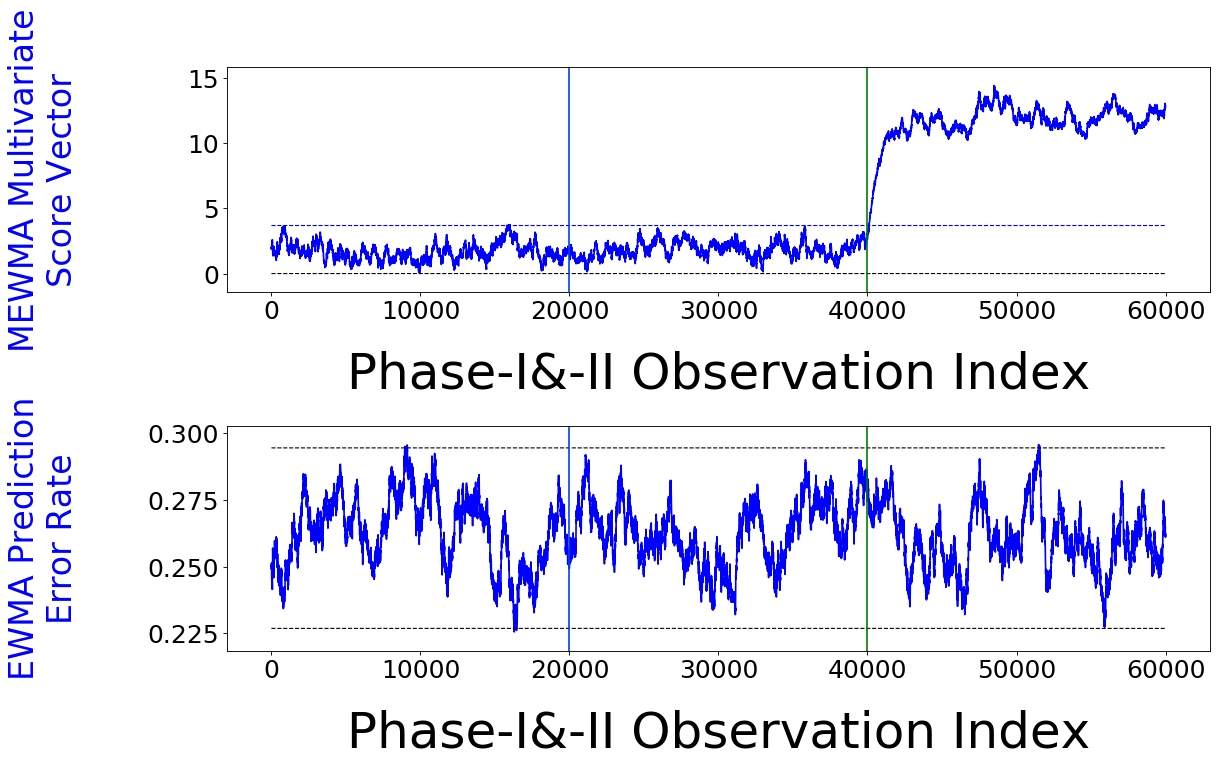
\includegraphics[width = .8\linewidth]{./figures_archive/sim_11/non_nnet_nonunif_ch_f_0_2/1_sim11_logi_1e-08_0_0015_1.png}
  \caption{Illustration of concept drift detection performance for a logistic regression example in which the change in $\bm{\theta}$ results in no change in the error rate. The $1$st~(blue) vertical line is the boundary between the Phase-I~(to the left of the line) and Phase-II data~(to the right of the line), and the $2$nd~(green) vertical line indicates when $\bm{\theta}$ changed. The top plot is the score-based MEWMA, and the bottom plot is the EWMA on the error rate. The score-based approach effectively detects the concept drift, even though there is no change in error rate.}
  \label{fig_CD:exp_no_err_ch}
\end{figure}
In Section~\ref{ss_CD:score_func}, we gave a simple logistic regression example~(see Figure~\ref{fig_CD:logi_err_rate_unch}) in which there is concept drift, but the concept drift does not result in a change in error rate. Consequently, methods based on monitoring the error rate will fail to detect the concept drift, whereas our score-based approach can still detect the drift. We return to this example and show the monitoring performance of both methods over a set of simulated data generated from the logistic regression model similar to~(\ref{eqn_CD:logi_mod_score})~(here, the dimension of parameters $\bm{\theta}$ is $3$) with $\bm{\theta}^{(0)} = [0,2,2]^T$ prior to the concept drift and $\bm{\theta}^{(1)} = [0.2,2.4,4.4]^T$ following the concept drift. The logistic regression model was fitted and the control limits computed via the procedure described in Section~\ref{ss_CD:MEWMA}, using simulated training and Phase-I data, respectively. We used a desired false alarm rate of $\alpha=0.001$. Figure~\ref{fig_CD:exp_no_err_ch} shows the monitoring results over both the Phase-I and Phase-II data. The latter were also generated from the same logistic regression model with parameters $\bm{\theta}^{(0)}$ up until the parameters changed at observation index around $40000$, after which the remainder of the Phase-II data were generated using parameters $\bm{\theta}^{(1)}$. As seen in Figure~\ref{fig_CD:exp_no_err_ch}, our score-based MEWMA promptly detects the concept drift, whereas the EWMA on the error rate does not detect it. 

If the concept drift does not cause a change in the error rate, one might wonder whether it is important to detect the concept drift. The answer is ``yes", because it indicates to the user that there is an opportunity to improve the model and further reduce the error rate. In the above example, using the predictive model with parameters $\bm{\theta}^{(1)}$, the mean error rate is $0.26$ before, as well as after, the parameters of the data generation model change from $\bm{\theta}^{(0)}$ to $\bm{\theta}^{(1)}$. However, after the concept drift is detected, if the parameters of the predictive model are updated to $\bm{\theta}^{(1)}$ by refitting the model to the new data, then the error rate will decrease substantially from $0.26$ to $0.15$.


\subsection{Credit Risk Modeling Example}
\label{ss_CD:cr_ds}
In the credit risk data set, each row corresponds to a unique credit card customer of a major financial company, and we have $196587$ rows of data in total. The covariates for row/customer $i$ include various customer information~($\bm {x}_i$) available at the time the customer applies for the credit account, and the binary response~($y_i$) indicates whether the customer defaults within the first $9$-month after opening the account. For the purposes of plotting various quantities over time, we associate each row $i$ with a time stamp that is taken to be the day on which the response $y_i$ first becomes available. Specifically, the set of all customers associated with a particular day, which we refer to as their ``entry day" into the data set, are those who opened their account within nine months of that day and defaulted on that day~(in which case they are assigned $y_i=1$), together with those who opened their account exactly nine months prior to that day and did not default~(in which case they are assigned $y_i=0$). The data are imbalanced in the sense that there are $3536$ observations with $y_i = 1$, which accounts for around $1.8\%$ of the data. Consequently, when fitting the model to the training data, we assign a weight of $7.5$ to the minority class~(which corresponds to upsampling the minority class by a factor of $7.5$) so that the weighted percentage of the minority class in training data is around $10\%$. For the training, validation, Phase-I, and Phase-II data sets, the classification errors and score vectors in Equation~(\ref{eqn_CD:score_func}) and any quantities related to them are also using the same weighting scheme. That is, for each minority-class observation, its score vector in the MEWMA equation in Equation~(\ref{eqn_CD:ewma}) is multiplied by $7.5$, its Hessian and score vector are multiplied by $7.5$ when computing the average Hessian~(for Fisher decoupling) and average score vector~(for use in the Hotelling $T^2$ statistic~(\ref{eqn_CD:hotellingt2})), etc. 

These data were originally considered in~\cite{im2012time}, who focused on the same $10$ covariates that we consider in this study: $x_1$~(credit risk score from an earlier model used by the company), $x_2$~(credit bureau risk score), $x_3$~(highest credit limit for open revolving credit accounts), $x_4$~(total balance on all open revolving credit accounts), $x_5$~(balance on the highest-utilization open revolving credit account), $x_6$~(credit limit on the highest-utilization open revolving credit account), $x_7$~(number of inquiries in the last $24$ months), $x_8$~(balance on open mortgages), $x_9$~(categorical variable involving status of savings accounts), and $x_{10}$~(number of inquiries in the last $24$ months, excluding the last two weeks). 

We applied concept drift detection to two supervised learning models:  A logistic regression model and a neural network~(with one hidden layer having $50$ activation nodes). The main reason the company fits models of this nature was to score credit card applicants for risk~(via their predicted probability of defaulting) at the time they apply. For the purpose of evaluating the concept drift detection, we trained and validated both models on the data from $2003$-Jan to $2005$-Dec. The data from $2006$-Jan to $2006$-Dec are used as the Phase-I data to calculate control limits. The remainder of the data, from $2007$-Jan to $2008$-Aug are used as the Phase-II data to test the capability of detecting the concept drift due to the subprime mortgage crisis. Recall that the S\&P $500$ declined by more than $50\%$ over a $15$-month period between the end of $2007$-Dec and the end of $2009$-Mar~(from $1478$ to $683$). The prevailing view is that the major root cause of the stock market decline was the subprime crisis, which had been gradually developing prior to that.

We applied our score-based MEWMA with the goal of detecting concept drift as far in advance of the beginning of the crash~($2007$-Dec) as possible. For comparison, we also applied an EWMA on the (weighted) binary classification error. The predicted label, used to calculate the binary classification error, is $1$ if the predicted probability exceeds a specified threshold, and $0$ otherwise). We chose a threshold of $0.1057$ to match the true positive rate and the true negative rate as closely as possible~(alternatively, if costs of false positives and false negatives were known in advance, we could have chosen the threshold to minimize the total misclassification cost). For both methods, we selected $\lambda = 0.001$, so that the effective window is $\frac{1}{\lambda} = 1000$ customers, which corresponds roughly to one week. Figure~\ref{fig_CD:credit_default} shows the results of both concept drift monitoring methods for both models~(logistic regression and neural network) over the Phase-I and Phase-II data. 

As seen in Figure~\ref{fig_CD:credit_default}, for the logistic regression model, the score-based MEWMA consistently signals~(i.e., the $T^2$ statistic consistently falls above the $UCL$ ) beginning around $2007$-Mar, which is about $9$ months prior to the beginning of the economic crash in $2007$-Dec. In this sense, the score-based approach provides advanced warning that something has changed substantially in the predictive relationship between $Y$ and $\bm{X}$, which could have been indicative that serious economic changes were evolving. At the very least, it would have been an indication that the fitted credit risk scoring model was becoming obsolete and that more effective scoring could be achieved by updating the model. In contrast, the EWMA on the error rate does not consistently signal until much later, around $2008$-Jan, which is $10$ months after the score-based MEWMA began to consistently signal and $1$ month after the economic crash began. The results for the neural network model, which  are shown in the right panels of Figure~\ref{fig_CD:credit_default}, are very similar. 

\begin{figure}[!htbp]
\centering
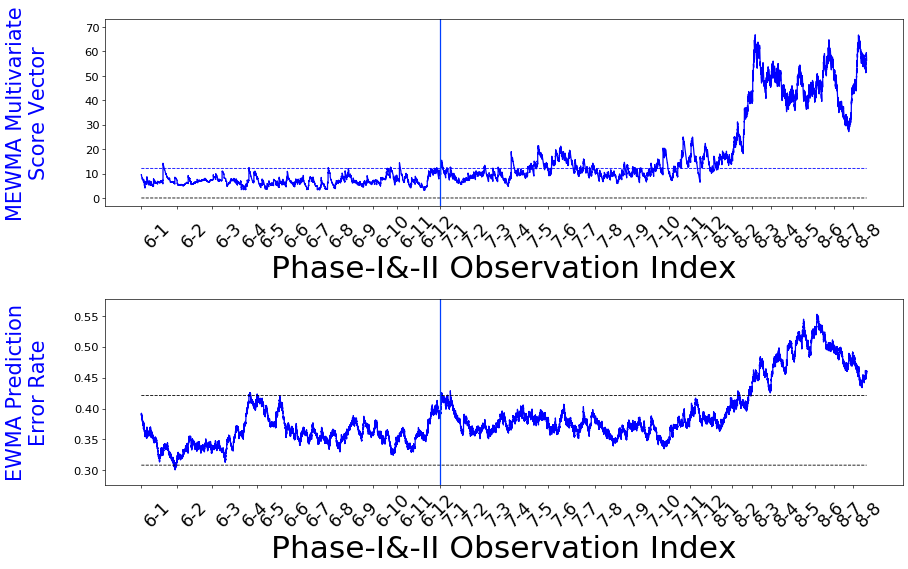
\includegraphics[width = 0.49\linewidth]{./figures_archive/credit_default/logi_scal_PI_train_sample_weights/credit_logi_1e-08_0_0001_0_001_99_0.png}
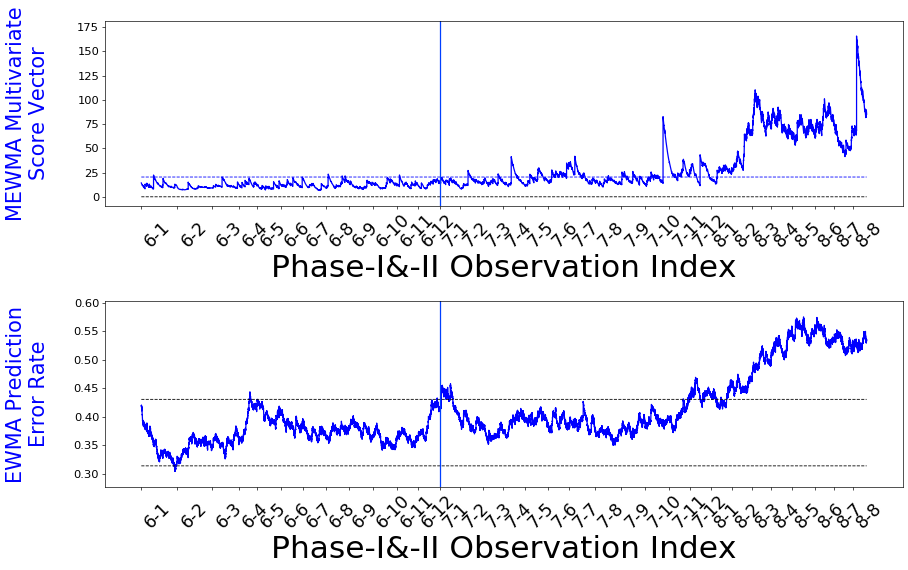
\includegraphics[width = 0.49\linewidth]{./figures_archive/credit_default/logi_nnet_50_scal_PI_train_sample_weights/credit_logi_1e-07_0_0001_0_001_99_0.png}
  \caption{
For the credit risk example, comparison of concept drift monitoring performance for our score-based MEWMA~(the top plots) versus an EWMA on the classification error~(the bottom plots). The left and right plots are for the logistic regression and neural network models, respectively. The blue blue vertical line is the boundary between the Phase-I and Phase-II data. The tilted numbers along the horizontal axes below each plot are the year-month indices~(e.g., $6$-$1$ stands for 2006-Jan). The score-based MEWMA consistently signals beginning $2007$-Mar, which is nine months prior to the beginning of the stock market crash in $2007$-Dec. In contrast, the EWMA on the classification error does not consistently signal until around $2008$-Jan. 
}
\label{fig_CD:credit_default}
\end{figure}

Figure~\ref{fig_CD:credit_default_diag} shows several representative univariate component EWMA control charts~(for $\theta_1$, $\theta_2$, $\theta_3$, $\theta_8$, and the intercept $\theta_0$) for the logistic regression model over the Phase-I and Phase-II data. The MEWMA is also shown in the top row as a reference. The component EWMA control charts in the left column are for the original~(coupled) score components~(\ref{eqn_CD:uniewma}), and those in the right column are for the Fisher-decoupled score components~(\ref{eqn_CD:uniewma-decoupled}) using the Hessian matrix version of $\widetilde{\mathbb {I}}(\bm { \theta}^{ (0)})$ for decoupling $\Delta \tilde{\bm { \theta}}$ via~(\ref{eqn_CD:decouple-2}). Rather than estimating the Fisher information matrix as the sample covariance matrix as in Equation~(\ref{eqn_CD:decouple}), we used its theoretical Fisher information matrix expression for logistic regression.

Decoupling the score components reveals different patterns of concept drift than are seen in the original score components. In particular, the decoupled component EWMA for the intercept parameter~(the bottom right plot) shows a clear upwards drift over the entire range of data, whereas this drift is not apparent in the corresponding original component EWMA~(the bottom left plot). The correlation between the intercept term and some of the other covariates has evidently conflated the drift in their corresponding parameters in the left column plots. The upwards drift in the decoupled intercept parameter is telling, as the intercept can be viewed as a regression-adjusted indicator of the overall default rate. Since the drift was upwards, this means that the intercept parameter increased over time, which means that the regression-adjusted likelihood of default~(i.e., the default for applicants having the same covariate values) increased substantially over time. In fact, the concept drift may even be evident earlier in the decoupled component EWMA for $\theta_0$ than in the MEWMA. For example, the decoupled component EWMA for $\theta_0$ falls consistently above the center line~($0$) beginning back in the Phase-I data, around $2006$-Jun. Even though it is not above the $UCL$ at this point, the fact that it is consistently above the center line is an indication that $\theta_0$ has increased. In SPC control charting in general, users typically look for these types of patterns in the charts to signal changes in the mean of what is being charted~(\cite{montgomery2007introduction}). 

The decoupled component EWMA chart for $\theta_1$~(the right column, the $2$nd from top) also shows a clear downwards drift in $\theta_1$, which means that $x_1$~(credit risk score from an earlier model) should be given less weight in predicting credit risk as time evolves. This makes sense, because the earlier model had been fitted to even earlier data.  The decoupled component EWMA chart for $\theta_2$~(the right column, the $3$rd from top) has a different trend that is also less extreme than for $\theta_1$. It is interesting that the component EWMA charts for $\theta_1$ and $\theta_2$ prior to decoupling~(second and third plots in the left column) are far more similar than their decoupled counterparts. This is likely because $x_1$ and $x_2$ have a correlation coefficient of $0.45$, and correlation between covariates conflates the concept drift in their coefficients, whereas the Fisher decoupling is intended to distinguish the concept drift in the coefficients.    



\begin{figure}[H]
\centering
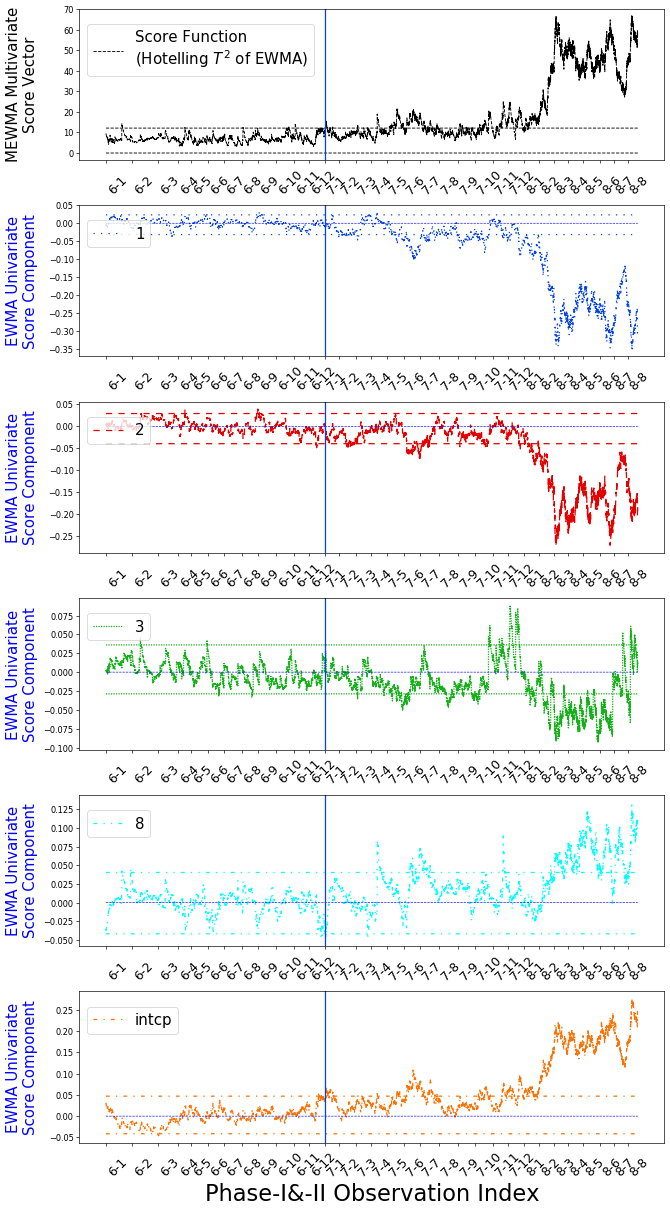
\includegraphics[width = 0.48\linewidth]{./figures_archive/credit_default/logi_scal_PI_train_sample_weights/pos_single_credit_mlines_with_regu_1e-08_0_0001_0_001_99_0.png}
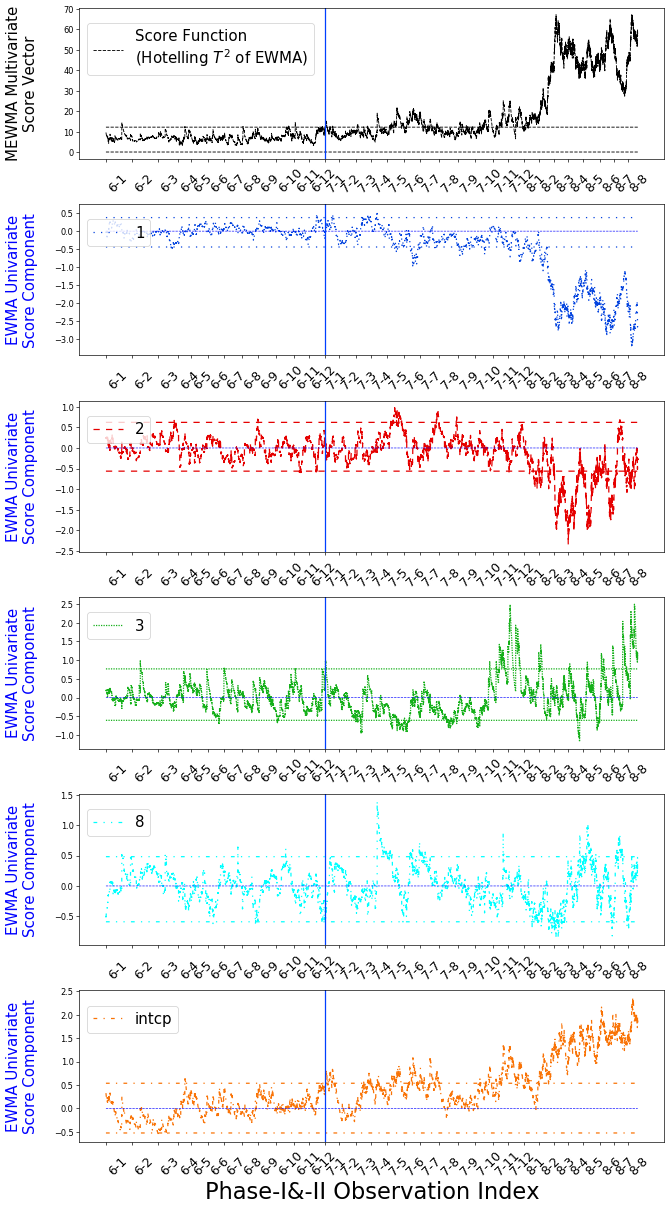
\includegraphics[width = 0.48\linewidth]{./figures_archive/credit_default/logi_scal_PI_train_sample_weights/pos_single_credit_fisher_mlines_with_regu_1e-08_0_0001_0_001_99_0.png}
\caption{
MEWMA~(the top row) and various univariate component EWMA~(the other rows, for $\theta_1$, $\theta_2$, $\theta_3$, $\theta_8$, and the intercept $\theta_0$) control charts for the logistic regression model in the credit risk example over the Phase-I and Phase-II data. The left column are the original score component EWMA control charts~(\ref{eqn_CD:uniewma}), and the right column are the decoupled component EWMA control charts~(\ref{eqn_CD:uniewma-decoupled}). The horizontal lines are the control limits and also a line indicating the zero value for the EWMAs. The blue vertical line is the boundary between the Phase-I and Phase-II data. The decoupled component EWMA control charts show clear drift in a number of parameters, especially the intercept~(the bottom right) and $\theta_1$~(the second from the top, the right column).
}
\label{fig_CD:credit_default_diag}
\end{figure}

\subsection{Bike Sharing Rental Count Modeling Example}
\label{ss_CD:bs_ds}

The bike sharing data set\footnote{https://www.capitalbikeshare.com/system-data} comes from hourly-aggregated loggings of the Captial Bikeshare system in $7$ jurisdictions of the Washington metropolitan area from $2010$--$2020$, integrated with hourly weather data\footnote{https://www.freemeteo.com} over the same time period. The total sample size is $n=82093$, and each row corresponds to one hour, with the response~($y$) being the number of bike rentals during that hour, and the covariates~($\bm {x}$) being time- and weather-related variables for that hour. We use the same definitions and preprocessing procedures described for the UCI data set\footnote{https://archive.ics.uci.edu/
ml/datasets/Bike+Sharing+Dataset}~(\cite{fanaee2014event}). The $d=10$ covariates are year~($x_1$, numerical with $11$ integer values from $2010$ to $2020$), month~($x_2$, categorical with $12$ categories: $1=Jan, 2=Feb, \cdots, 12=Dec$), hour~($x_3$, categorical with $24$ categories: $\{0,1,\cdots,23\}$), holiday~($x_4$, binary: $0=non\text{-}holiday,1=holiday$), weekday~($x_5$, categorical with $7$ categories: 
$0=Sun,1=Mon,\cdots,6=Sat$), workingday~($x_6$, binary: $0=weekend~or~holiday,1=otherwise$), weather situation~($x_7$, categorical with $3$ categories: $1 = \{clear|few~clouds|partly~cloudy\}, 2=\{cloudy|misty\}, 3=\{rain|thunder|snow|freezing~fog\}$), temp~($x_8$, numerical: temperature in Celsius), hum~($x_{9}$, numerical: humidity), and windspeed~($x_{10}$, numerical: wind speed). Several of the original covariates were dependent on others~(e.g., season is a deterministic function of month; feeling temperature is highly correlated with temp) and so were excluded from the model. See~\cite{apley2020visualizing} for an analysis of these data and graphical illustrations of the main effects and interaction effects of the various covariates via accumulated local effects plots.

In the following, we fitted and tuned various regression models on windows of data. In each case, we used the data for the one year following the training data~(see results in this section below for details) as the Phase-I data for establishing the control limits, and we used the remainder of the data following the Phase-I data as our Phase-II for the prospective concept drift detection. In all cases, we chose the EWMA parameter $ \lambda = 0.01$, which corresponds to an effective window length of $\frac{1}{\lambda}=100$ or a little over half a week. We standardized all numerical covariates and responses to have a range of approximately $[0,1]$. For the linear regression model, we included interactions between selected pairs of covariates~(i.e., month, weekday, and holiday respectively interacting with hour; month interacting with weekday; month, weekday, hour, temp, hum, and windspeed respectively interacting with weather situation; temp interacting with windspeed) based on intuitions and manual step-wise regression, and we included quadratic terms for the numerical covariates, which resulted in a $5$-fold cross-validation~(CV) error of $r^2_{\mathrm{CV}} \approx 0.87$, and this was consistent between the \texttt{R} package \texttt{glmnet} and the \texttt{python} package \texttt{sklearn}. For the neural network model, we used two hidden layers with $10$ and $5$ nodes and the logit output. Since all the categorical covariates truly ordinal (although we treated them as nomial in the logistic regression) or binary and a neural network can capture nonlinear trends across a numerical covariate, we converted all categorical covariates to numerical for the neural network. The $5$-fold $r^2_{\mathrm{CV}} \approx 0.94$ was consistent between the \texttt{python} package \texttt{tensorflow} and the \texttt{R} package \texttt{nnet}~(for \texttt{nnet} we can only use one hidden layer, for which we chose $20$ nodes and the logit output). 

To illustrate how we anticipate someone using our score-based concept drift framework retrospectively and prospectively, consider the hypothetical situation where we are an analyst with the bike-sharing company, it is currently $2018$-Jan, and we have just collected past data through the end of $2017$-Dec. Our first objective is to conduct a retrospective analysis on the past data to determine if the predictive relationship $P(Y|\bm{X})$ was stable over the entire $2010$-Sep through $2017$-Dec range. If $P(Y|\bm{X})$ was stable, then we intend to fit our predictive model over the $2010$-Sep through $2016$-Dec range as the training data, determine the score-based MEWMA and component EWMA control limits from the $2017$-Jan through $2017$-Dec range as the Phase-I data, and then prospectively monitor the data for concept drift beginning $2018$-Jan as the Phase-II data. On the other hand, if the retrospective analysis indicates that $P(Y|\bm{X})$ was not stable over the entire $2010$-Sep through $2017$-Dec range, then the objective is to conduct diagnostics to identify the reasons why and take appropriate actions based on that~(e.g., modifying the model or fitting it to a narrower, more recent window of data).

Figure~\ref{fig_CD:bs_retro} shows retrospective diagnostic plots for a linear regression model. The top plot is the MEWMA, and the other plots are the Fisher-decoupled component EWMA control charts~(\ref{eqn_CD:uniewma-decoupled}) for various parameters using the $\Delta \tilde{\bm { \theta}}$ decoupling Equation~(\ref{eqn_CD:decouple-2}) with the theoretical expression for the Fisher information matrix $\widetilde{\mathbb {I}}(\bm { \theta}^{ (0)})$. There is clearly concept drift over this period, which is most evident from the MEWMA and the component EWMA control charts for the year and intercept parameters. To see the drift more clearly, it is helpful to redo the retrospective plots but with the training and Phase-I data changed to a narrower window over which $P(Y|\bm{X})$ drifted less. This is shown in Figure~\ref{fig_CD:bs_retro_narrow_train}, for the training window $2012$-Jun to $2015$-Jun, which represents the middle of the full $2010$-Sep to $2017$-Dec data range. The control limits become narrower and the drift is more apparent in Figure~\ref{fig_CD:bs_retro_narrow_train}. In particular, it appears that the year parameter should be higher in the earlier years and lower in the later years, and the intercept parameter should also be lower in the later years. This is consistent with the overall growth trend in bike rentals over the time period, which is not quite linear. Figure~\ref{fig_CD:bs_retro_narrow_train} also indicates other seasonality phenomena that the model is unable to capture and that appear to be amplified outside of the narrower training window, perhaps also due to the growth trend.  

\begin{figure}[H]
\centering
    \begin{subfigure}[t]{0.33\linewidth}
     \centering
         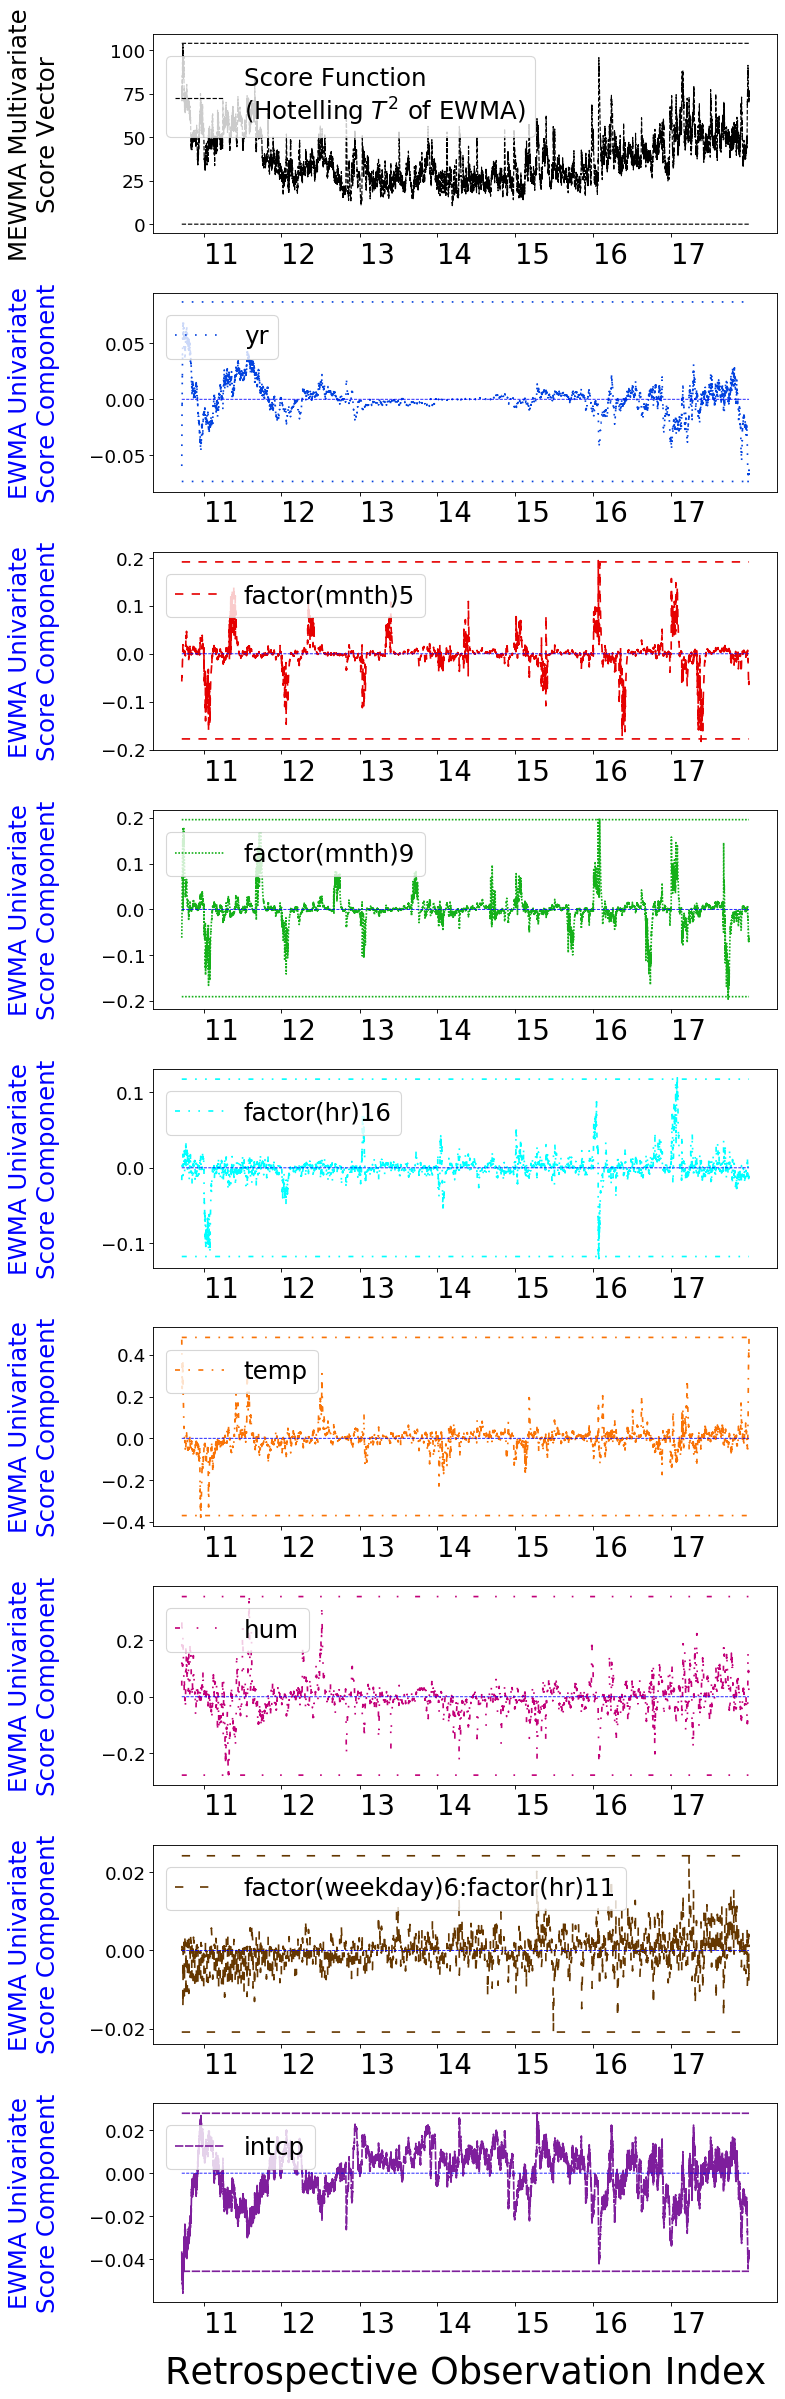
\includegraphics[width=1.0\textwidth, trim=.0in .0in .0in .0in, clip]{./figures_archive/bike_sharing/reg_lin_A/quadr/PII_pos_single_retro_bike_fisher_mlines_with_regu_1e-08_0_0001_0_01_99_99.png}
     \captionsetup{width=.95\linewidth}
     \caption{}
     \label{fig_CD:bs_retro}
\end{subfigure}
\begin{subfigure}[t]{0.33\linewidth}
     \centering
         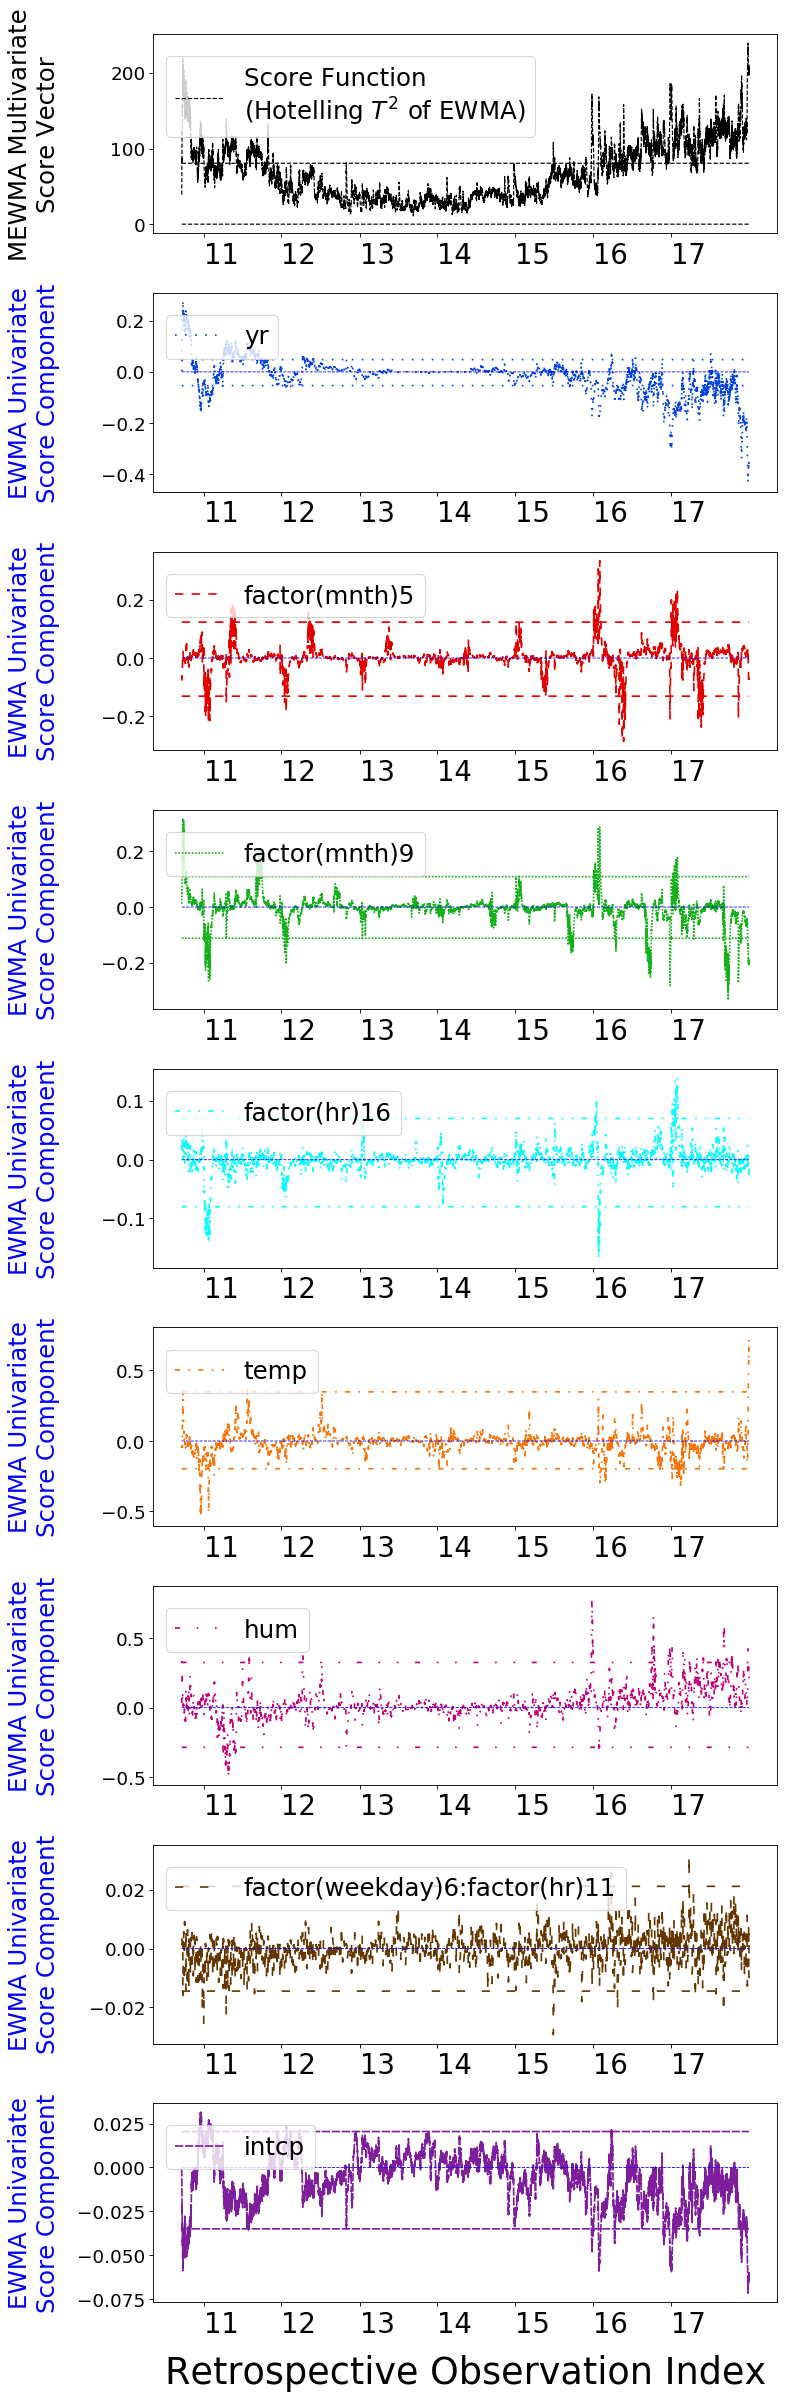
\includegraphics[width=1.0\textwidth, trim=.0in .0in .0in .0in, clip]{./figures_archive/bike_sharing/reg_lin_B_1/quadr/PII_pos_single_retro_bike_fisher_mlines_with_regu_1e-08_0_0001_0_01_99_99.png}
     \captionsetup{width=.95\linewidth}
     \caption{}
     \label{fig_CD:bs_retro_narrow_train}
\end{subfigure}
\caption{Retrospective diagnostic charts for a linear regression model with the original bike rental counts as the response. The top plots are the MEWMAs, and the other plots are the decoupled component EWMA control charts for various parameters. The training data are (a) from $2010$-Sep to $2017$-Dec and (b) from the narrower window $2012$-Jun to $2015$-Jun. In both cases, the Phase-I data used to determine the control limits are the same as the training data. These clearly indicate concept drift over the $2010$-Sep to $2017$-Dec period.}
\label{fig_CD:bike_sharing}
\end{figure}

To account for the growth trend, we modified the linear regression model by replacing the response variable $y$ with a normalized version  $y \leftarrow y/y_{\mathrm{MA}}^\beta$, where $\beta$ is a tuning parameter, and $y_{\mathrm{MA}}$ is the average rental count over an one-year, trailing, moving average window. We chose $\beta=0.78$ as the value that maximized the $r^2$ over the range from $2010$-Sep to $2017$-Dec with the model trained over the range from $2012$-Jun to $2015$-Jun as we did in Figure~\ref{fig_CD:bs_retro_narrow_train}~(we refer to this as the ``retrospective $r^2$"). 
This normalized model not only substantially mitigated the concept drift as described below, but also resulted in much better predictive power over the future data, which we discuss shortly. In particular, the retrospective $r^2$ in Figure~\ref{fig_CD:bs_retro_narrow_train} was approximately $0.81$ for the model trained on the original $y$, versus approximately $0.91$ for the model trained on the normalized $y$~(but transforming $y$ back to its original unit to compute the $r^2$). 

The results analogous to Figure~\ref{fig_CD:bike_sharing} but for this normalized model are shown in Figure~\ref{fig_CD:bike_sharing_norm}. Figure~\ref{fig_CD:bs_norm_retro} show retrospective diagnostic MEWMA and decoupled component EWMA control charts when the training and Phase-I data are from $2010$-Sep to $2017$-Dec. From this, it appears that $P(Y|\bm{X})$ is much more stable for the normalized model, although from the MEWMA and component EWMA control charts for the year and intercept parameters, the first two years do appear different from the remaining years. Because of this, we omitted the first two years and repeated the retrospective analysis with the training and Phase-I data from $2013$-Jan to $2017$-Dec. The results are shown in Figure~\ref{fig_CD:bs_norm_retro_narrow}, from which it appears that there is little concept drift for the normalized model over the period $2013$-Jan to $2017$-Dec. The strong seasonality seen in Figure~\ref{fig_CD:bike_sharing} for some of the parameters has also been substantially mitigated in Figure~\ref{fig_CD:bs_norm_retro_narrow}, which provides additional confidence in the model.

Based on Figure~\ref{fig_CD:bs_norm_retro_narrow}, at the ``current" $2018$-Jan point in time in our hypothetical story, the analyst might conclude that the model can be used for prediction going forward and begin monitoring it in Phase-II to detect if the model remains stable or changes at some later point. This Phase-II analysis is depicted in Figure~\ref{fig_CD:bs_norm_prospective}, for which the training data was from $2013$-Jan to $2016$-Dec and the control limits were determined from the Phase-I data from $2017$-Jan to $2017$-Dec. Going forward from $2018$-Jan, it appears that $P(Y|\bm{X})$ did remain reasonably stable until around the middle of $2019$, at which time the year and intercept parameters appear to decrease and then increase. Based on this, the analyst might have concluded around the end of $2019$ that it was time to update the predictive model. Note that the test $r^2$ over the Phase-II data in Figure~\ref{fig_CD:bs_norm_prospective} is $0.88$ for the model fitted to the normalized $y$~(also after transforming $y$ back to its original unit to compute the $r^2$), compared to a test $r^2$ of $0.82$ for the model fitted to the original $y$, which provides further justification for the transformation.

\begin{figure}[H]
\centering
    \begin{subfigure}[t]{0.305\linewidth}
     \centering
         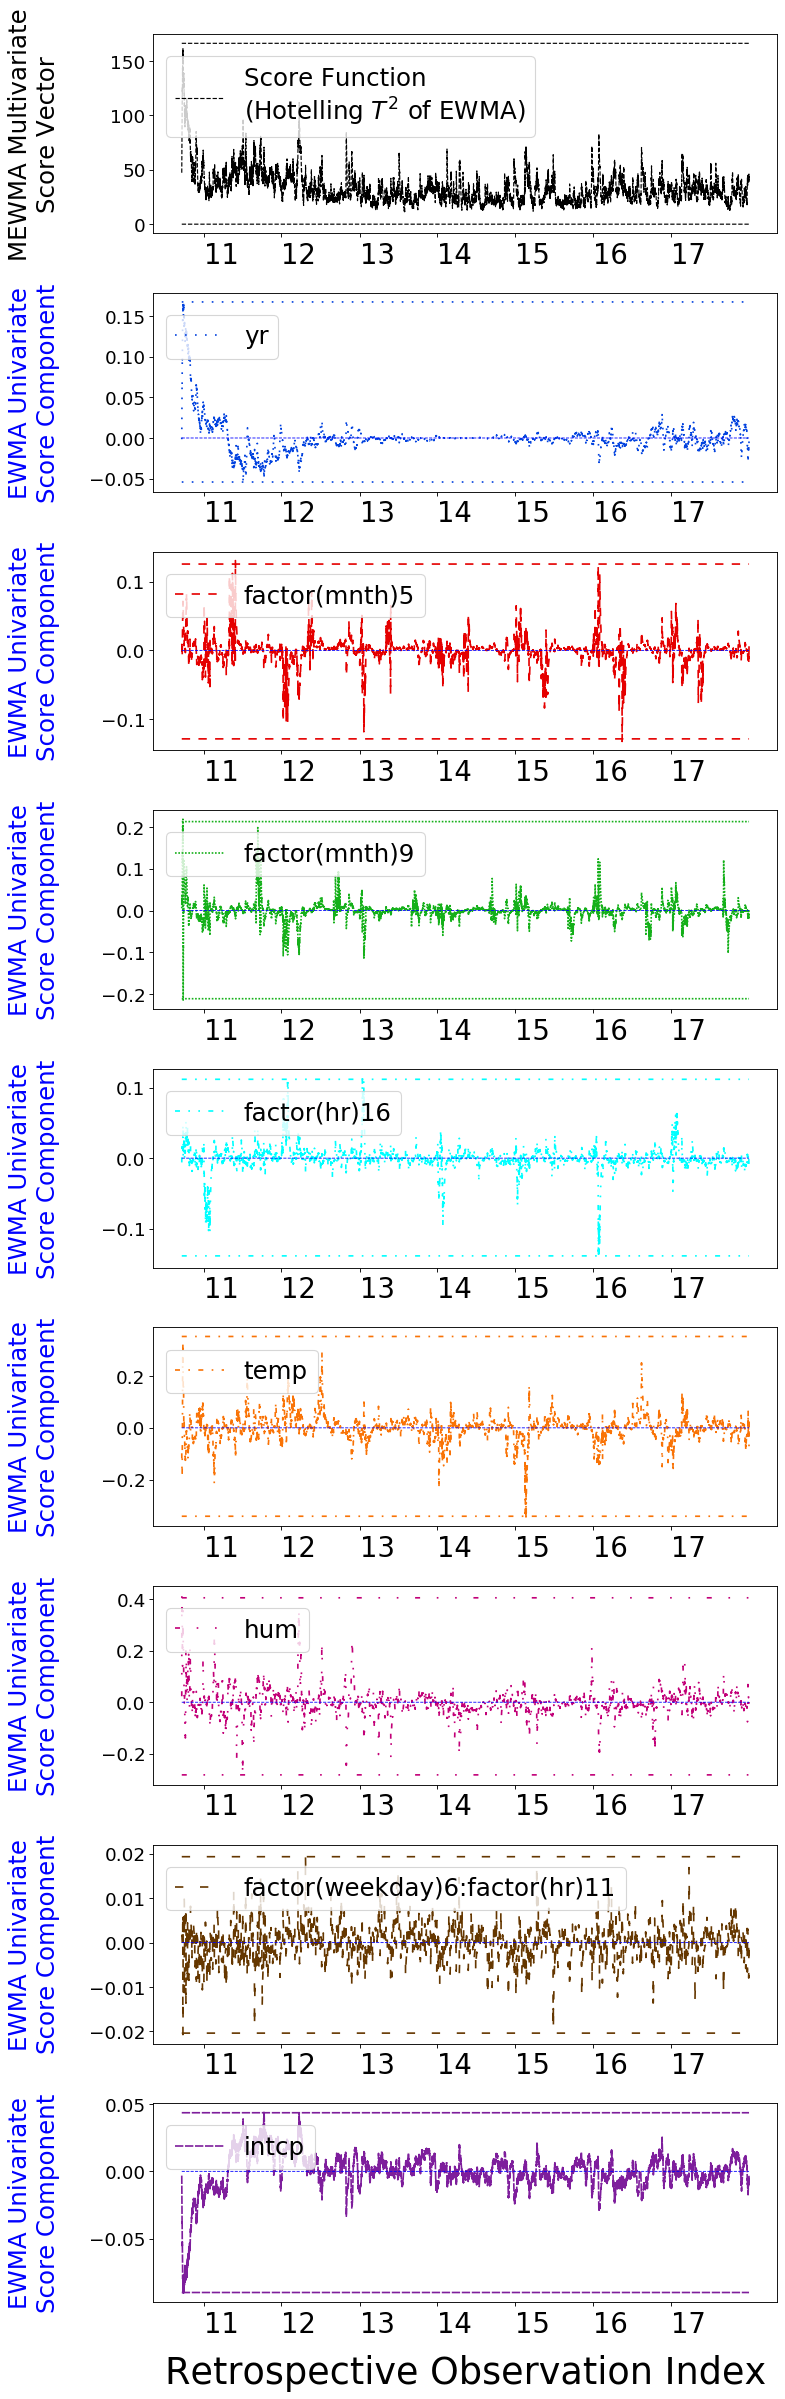
\includegraphics[width=1.0\textwidth, trim=.0in .0in .0in .0in, clip]{./figures_archive/bike_sharing/reg_lin_C/quadr/PII_pos_single_retro_bike_fisher_mlines_with_regu_1e-08_0_0001_0_01_99_99.png}
     \captionsetup{width=.95\linewidth}
     \caption{}
     \label{fig_CD:bs_norm_retro}
\end{subfigure}
\begin{subfigure}[t]{0.305\linewidth}
     \centering
         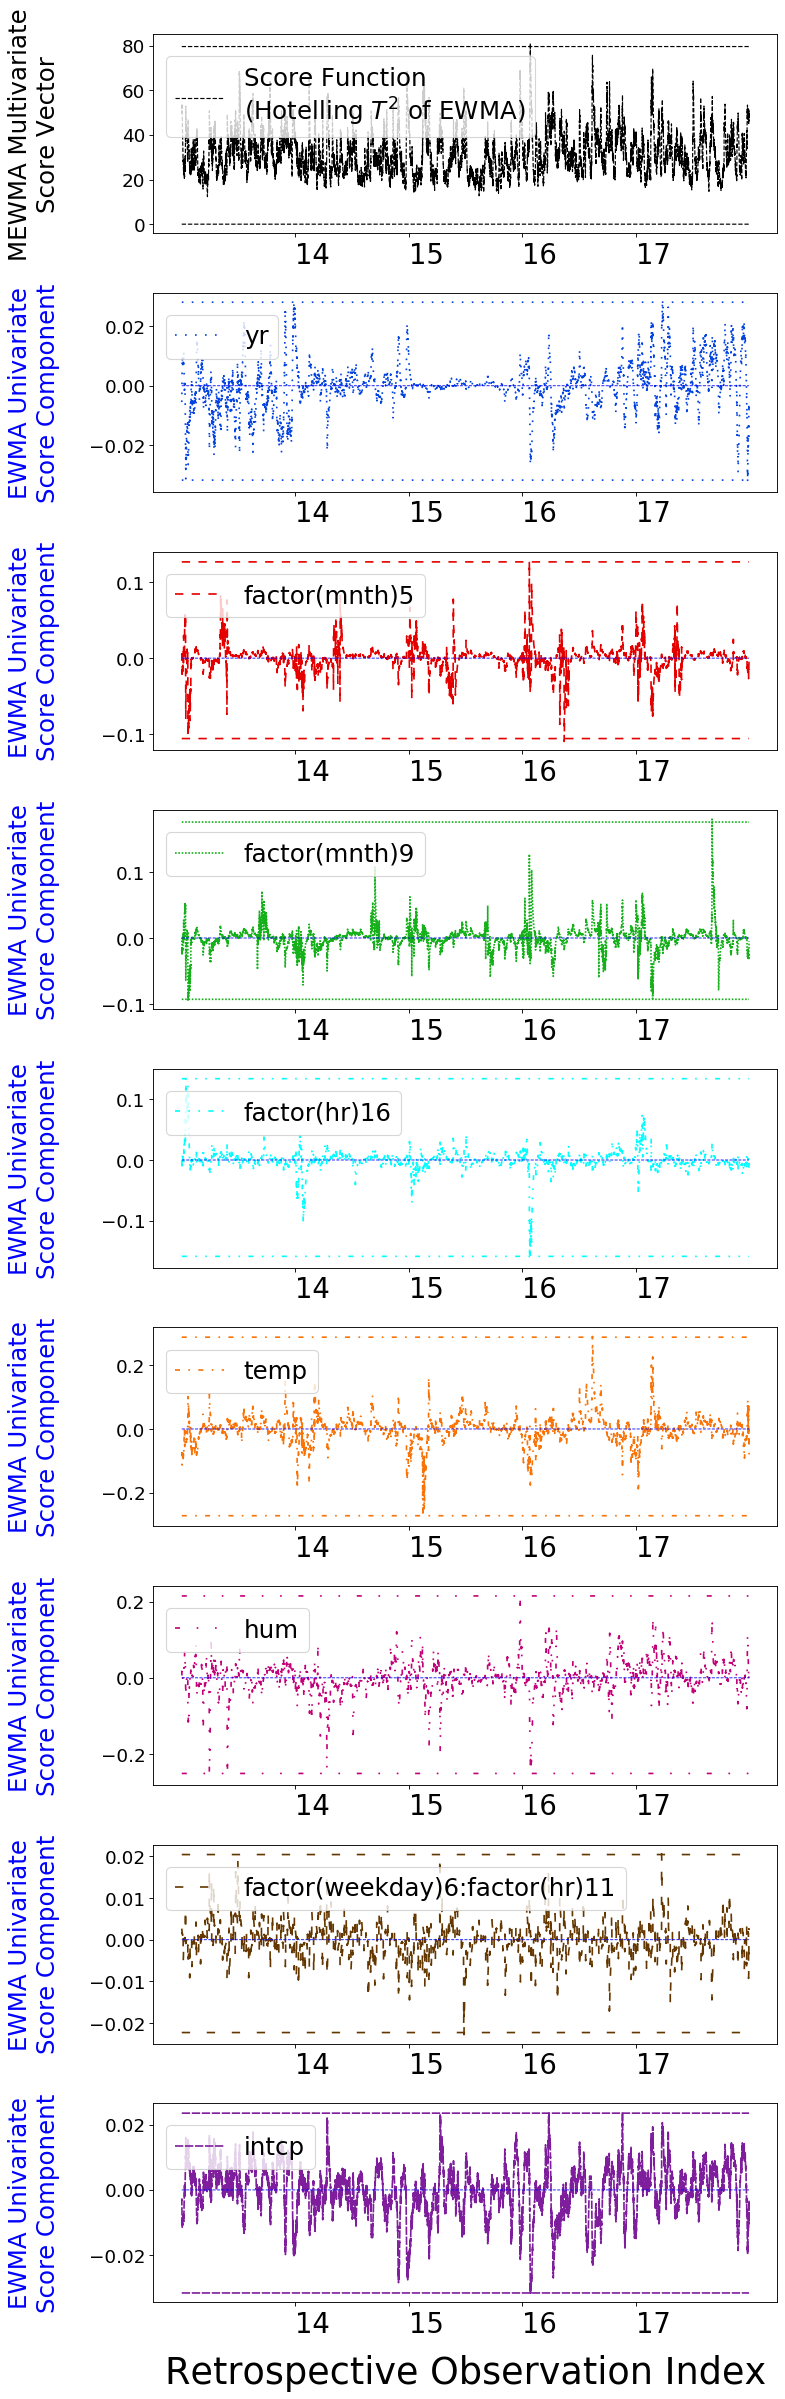
\includegraphics[width=1.0\textwidth, trim=.0in .0in .0in .0in, clip]{./figures_archive/bike_sharing/reg_lin_C_2/quadr/PII_pos_single_retro_bike_fisher_mlines_with_regu_1e-08_0_0001_0_01_99_99.png}
     \captionsetup{width=.95\linewidth}
     \caption{}
     \label{fig_CD:bs_norm_retro_narrow}
\end{subfigure}
\begin{subfigure}[t]{0.374\linewidth}
     \centering
         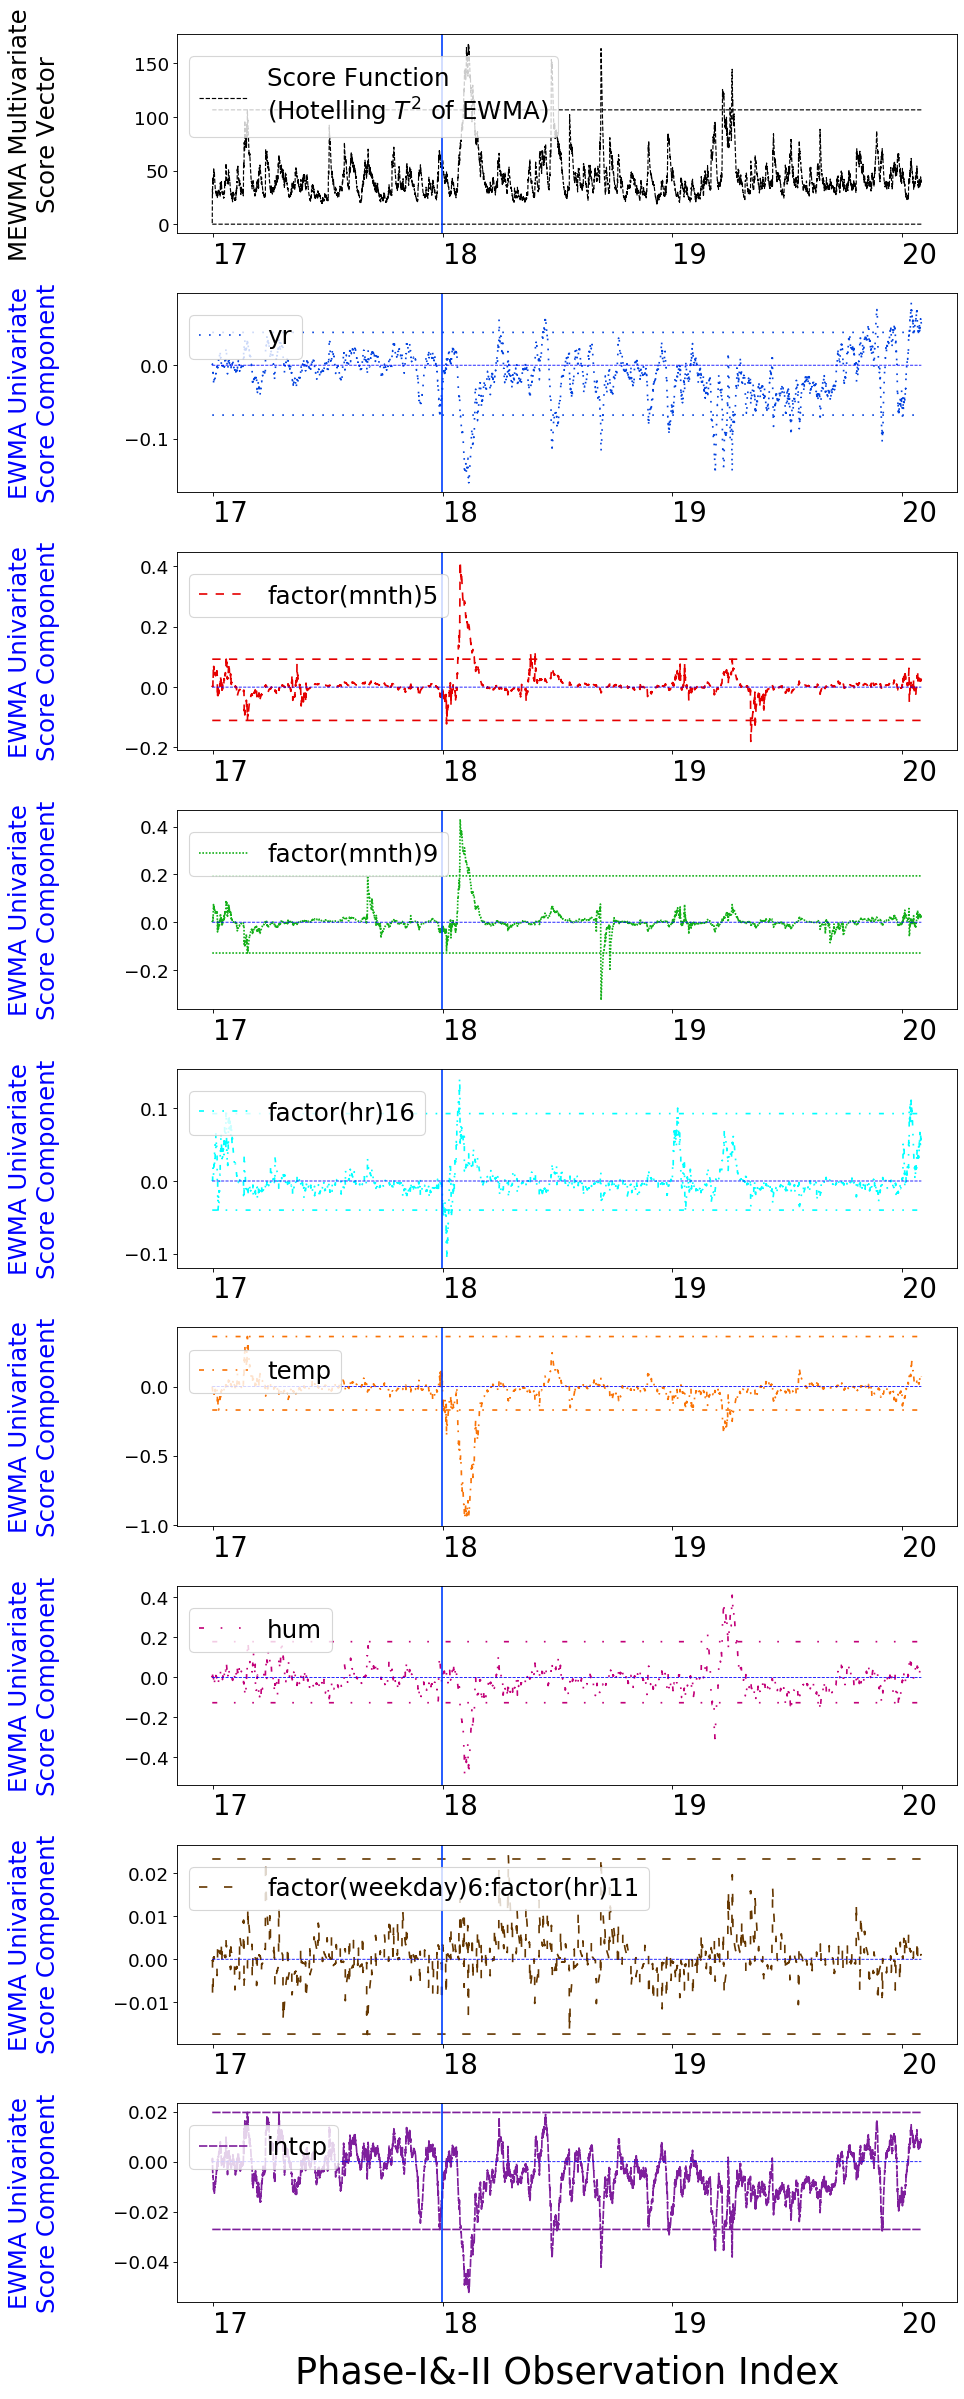
\includegraphics[width=1.0\textwidth, trim=.0in .0in .0in .0in, clip]{./figures_archive/bike_sharing/reg_lin_PI_D_2/quadr/pos_single_bike_fisher_mlines_with_regu_1e-08_0_0001_0_01_99_99.png}
     \captionsetup{width=.95\linewidth}
     \caption{}
     \label{fig_CD:bs_norm_prospective}
\end{subfigure}
\caption{Panels (a) and (b) are retrospective diagnostic MEWMA and decoupled component EWMA control charts for the linear regression model fit to the normalized bike rental counts. The training and Phase-I data are (a) from $2010$-Sep to $2017$-Dec and (b) from $2013$-Jan to $2017$-Dec. Panel (c) are prospective Phase-II MEWMA and decoupled component EWMA control charts for the same model with training period $2013$-Jan to $2016$-Dec and control limits determined from the Phase-I period $2017$-Jan to $2017$-Dec, with the vertical line delimiting the two periods. $P(Y|\bm{X})$ appears reasonably stable in Phase-II until around the middle of $2019$, at which time the year and intercept parameters appear to decrease and then increase.}
\label{fig_CD:bike_sharing_norm}
\end{figure}



\section{Conclusions}
Predictive models are trained on historical data sets, but due to potential changes in the conditional distribution $P (Y|\bm {X})$~(aka, concept drift) the performance of the models may degrade. We have developed a comprehensive, general, and powerful score-based framework for monitoring and diagnosing concept drift. The framework is general in that it applies to any parametric model, either regression or classification. It can be used retrospectively~(to analyze whether $P (Y|\bm {X})$ was stable over a past data set and aid in the model building procedure) and prospectively~(to quickly detect changes in $P (Y|\bm {X})$ so that predictive models currently in use can be updated accordingly). We have provided theoretical arguments that, under reasonably general conditions, concept drift occurs if and only if the mean of the score vector changes. Consequently, our score-based procedure is based on monitoring and analyzing changes in the mean of the score vector. For this, we have adopted procedures~(MEWMA and univariate EWMA) that were developed in the SPC literature for monitoring for changes in the mean of multivariate vectors in general. As part of the framework, we have also developed a diagnostic approach that involves decoupling changes in the parameters from the change in the mean of the score vector. 

In simulation and real data examples, we have demonstrated that our score-based monitoring procedure provides much more powerful detection of changes in $P (Y|\bm {X})$ than the state-of-the-art existing approach~(error-based EWMA). In particular, there are examples~(e.g., Figure~\ref{fig_CD:exp_no_err_ch}) in which the score-based approach quickly detects the change in $P (Y|\bm {X})$, but the error-based approach is completely unable to detect the change because they do not result in a change in the error rate. 


\vspace{1in}

\appendix
\label{appendices}
\bookmarksetupnext{level=part}

\setcounter{equation}{0}
\renewcommand{\theequation}{\thesection\arabic{equation}}
\setcounter{table}{0}
\renewcommand{\thetable}{\thesection\arabic{table}}
\setcounter{figure}{0}
\renewcommand{\thefigure}{\thesection\arabic{figure}}
\begin{appendices}

\section{Simulation Comparisons of Median Run-Length ($MRL$)}
\label{app:simu_MRL}
As mentioned in Section~\ref{s_CD:real_data}, we conducted MC simulations for simulated data sets generated from four GLM models~(logistic regression, multinomial regression, linear regression, and Poisson regression) to compare the $MRL$ of our score-based approach and the error-based methods. For each data set, $10$-dimensional covariates $\bm{x}$ are generated from a $10$ dimensional multivariate normal distribution with mean $\bm{0}$ and covariance matrix $\mathbf {I}$~(an identity matrix), and then, the response variable is generated from the respective GLM model, without an intercept term. The mathematical form of the models and their score vectors~(to be used in our control charts) are as follows.

\noindent
\underline{\textbf{Logistic regression}}:
\begin{align}
\begin{aligned}
P(Y=1|\bm{X};\bm{\theta}) =& \sigma ( \bm {X}^T\bm { \theta}) \\
\bm{s}(\bm { \theta};(\bm {X}, Y)) =&  (Y- \sigma (\bm {X}^T\bm { \theta} )) \bm {X},
\end{aligned}
\label{eqn_CD:logis_score}
\end{align}
where $ \sigma ( \cdot)$ is the sigmoid function.

\noindent
\underline{\textbf{Multinomial regression}}:
\begin{align}
\begin{aligned}
\ln \big(\frac{p_i}{p_0}\big) = \ln \big(\frac{P(Y=i|\bm{X};\bm{\theta})}{P(Y=0|\bm{X};\bm{\theta})}\big)&=\bm {X}^{T} \bm { \theta}_i, ~ i \in \{1,2,\cdots,K-1\} \\
\bm {s}(\bm { \theta} ; (\bm {X}, Y)) &= (\tilde{\bm{Y}}-\bm {p})\otimes \bm {X},
\end{aligned}
\label{eqn_CD:multi_score}
\end{align}
where $\bm { \theta} $ is generated by stacking all $ \bm { \theta}_i , (i=1,2,\cdots,K-1)$ into a $1$-dimensional vector; $\bm {p}=[p_1, p_2, \cdots, p _{K-1}]$; $\tilde{\bm{Y}}$ is the one-hot-encoding vector for $Y$, without the entry corresponding to label $0$; and $\otimes$ is the kronecker product.

\noindent
\underline{\textbf{Linear Gaussian regression}}:
\begin{align}
\begin{aligned}
P(Y=y|\bm{X};\bm{\theta})=& \frac{1}{\sqrt{2\pi\sigma^2}}\exp{\big\{-\frac{||y-\bm{X}^T\bm{\theta}||_2^2}{2\sigma^2} \big\}} \\
\bm{s}(\bm { \theta};(\bm {X}, Y)) =& (Y - \bm {X}^T\bm { \theta} ) \bm {X}.
\end{aligned}
\label{eqn_CD:lin_score}
\end{align}

\noindent
\underline{\textbf{Poisson regression}}:
\begin{align}
\begin{aligned}
P(Y=k|\bm{X};\bm{\theta})=&\frac{ \lambda ^{k} \exp(- \lambda)}{k!}, ~ k \in \{0,1,2,\cdots\} \\
s(\bm { \theta};(\bm {X}, Y))=& (Y- \lambda)\bm {X}
\end{aligned}
\label{eqn_CD:pois_score}
\end{align}
where we define the link function as $\ln \lambda = \bm {X}^T\bm{\theta}$.

For each data set, we fit their respective GLM model and also a neural network with a single hidden layer having $10$ nodes. The scores for the neural networks are calculated using back-propagation. We conduct $1000$ MC replicates for the neural network cases, due to their higher computational cost, and $10000$ MC replicates for the other cases.
For each data set, the size of training, validation, Phase-I, and Phase-II data are $10000$, $2000$, $20000$, and $20000$, respectively, in each replicate. 
To introduce multicolinearity, which is common in real situations, we made a modification that $x_5 \leftarrow 0.5x_1+0.5x_5$ and $x_6 \leftarrow 0.3x_2+0.3x_3+0.4x_6$ and all other covariates are not affected by this modification.

For each example, we considered three different sizes of parameter changes~(small, medium, and large) represented by $\xi$ (defined below). Since different values of the EWMA parameter $\lambda$ are effective at detecting different size changes, we also considered three different $\lambda$ values~(corresponding to the three different $\xi$ values) for each example, which we chose so that in Phase-II steady-state approximately $50\%$ of the Hotelling $T^2$ statistics fall above the $UCL$. To have a common basis for comparison, we chose the control limits for each method so that its $MRL_0$ was approximately equal to the same target value. The resulting values of $\lambda$ and $MRL_0$ varied across the examples and are listed in Tables~{\ref{tab:logi_MRL}--\ref{tab:pois_MRL}}, which also show the $MRL_1$ performance comparison results for the different methods. Note that a smaller $MRL_1$ is better and corresponds to earlier detection of concept drift. 

Details on the model parameters~(including the intercept and coefficients) used in all the examples are as follows. For all models, the intercepts are $0$~($\theta_0=0$). For logistic regression~(\ref{eqn_CD:logis_score}), all $10$ coefficients are $1$ ($\theta_i^{(0)}=1, i\in\{1,2,\cdots,10\}$). For multinomial regression~(\ref{eqn_CD:multi_score}), there are $5$ classes, and all coefficients in the form of a $4\times 10$ matrix $\mathbf{M}$ are~(the four rows are $\bm{\theta}_i$ for $i\in\{1,2,3,4\}$)
\begin{align}
\begin{aligned}
\mathbf{M} = 
\begin{bmatrix}
1 & 1 & 1 & 1 & 1 & 1 & 1 & 1 & 1 & 1\\
1 & 1 & -1 & 1 & 1 & -1 & 1 & 1 & -1 & 1\\
-1 & 1 & -1 & 1 & -1 & 1 & -1 & 1 & -1 & 1\\
1 & -1 & 1 & -1 & 1 & -1 & 1 & -1 & 1 & -1\\
\end{bmatrix},
\end{aligned}
\end{align}
and stacking all entries row-by-row forms $\bm{\theta}^{(0)}$.
For linear regression~(\ref{eqn_CD:lin_score}), all $10$ coefficients are also $1$~($\theta_i^{(0)}=1, i\in\{1,2,\cdots,10\}$) and $\sigma^2=1$. For Poisson regression~(\ref{eqn_CD:pois_score}), all $10$ coefficients are $0.3$~($\theta_i^{(0)}=0.3, i\in\{1,2,\cdots,10\}$). The Phase-II observations are generated with the following changes in $\bm{\theta}$. The first four coefficients of logistic regression, linear regression, Poisson regression, and the first row of $\mathbf{M}$ for multinomial regression are multiplied by $1-\xi$~(e.g., for logistic regression, $\theta_i^{(1)}=(1-\xi)\theta_i^{(0)}, i\in\{1,2,3,4\}$ and $\theta_i^{(1)}=\theta_i^{(0)}, i\in\{5,6,\cdots,10\}$), where $\xi\in(0,1)$ governs the size of the concept drift~(larger $\xi$ means larger concept drift).

It can be seen from Tables~\ref{tab:logi_MRL}--\ref{tab:pois_MRL} that for all of our examples, the score-based method virtually always has smaller $MRL_1$'s than the error-based methods, especially for small drifts. The only exceptions are two cases in Table~\ref{tab:lin_MRL} for large $\lambda$, for which the $MRL_1$ values are virtually the same.
The gap between $MRL_1$'s of the score-based metric and other metrics is often quite substantial, especially when concept drift size is smaller and thus more challenging to detect. These results indicate the generality and superior performance capability of the score-based method.

\begin{table}[H]
\centering
\begin{tabularx}{\textwidth}{l*{1}c*{7}{Y}} %
\toprule
\multicolumn{2}{c}{\multirow{2}{*}{($ \xi$, $ \lambda$)}} & \multicolumn{3}{c}{Logistic regression model} & \multicolumn{3}{c}{Neural network model} \\ \cmidrule(l){3-8}
\multicolumn{2}{c}{} & {$  \lambda_1^{\text{glm}}$} & {$ \lambda_2^{\text{glm}}$} & {$ \lambda_3^{\text{glm}}$} & {$  \lambda_1^{\text{nn}}$} & {$ \lambda_2^{\text{nn}}$} & {$ \lambda_3^{\text{nn}}$} \\
\toprule
\multirow{2}{*}{$MRL_0$ ($\xi = 0$)} & score &$3500.0$ & $3499.0$ & $3502.5$ &$3494.0$ & $3505.5$ & $3494.5$\\
& error &$3499.5$ & $3501.0$ & $3500.0$ &$3503.5$ & $3508.0$ & $3521.5$ \\
\midrule
\midrule
\multirow{2}{*}{$MRL_1$ ($\xi = 0.3$)} & score &$\bm{391.0}$ & $\bm{377.5}$ & $\bm{464.0}$ &$\bm{476.0}$ & $\bm{390.0}$ & $\bm{385.0}$\\
& error &$835.0$ & $1050.0$ & $1278.0$ &$800.5$ & $834.5$ & $1064.0$ \\
\midrule
\multirow{2}{*}{$MRL_1$ ($\xi = 0.5$)} & score &$\bm{184.0}$ & $\bm{148.0}$ & $\bm{153.0}$ &$\bm{252.5}$ & $\bm{177.0}$ & $\bm{153.5}$ \\
& error &$359.0$ & $360.5$ & $442.0$ &$403.0$ & $346.5$ & $349.5$ \\
\midrule
\multirow{2}{*}{$MRL_1$ ($\xi = 0.7$)} & score &$\bm{111.0}$ & $\bm{82.0}$ & $\bm{75.0}$ &$\bm{159.0}$ & $\bm{110.0}$ & $\bm{84.0}$\\
& error &$205.0$ & $177.0$ & $186.0$ &$251.0$ & $198.0$ & $177.0$ \\
\midrule
\end{tabularx}
\caption{Comparison of $MRL_1$'s for our score-based MEWMA~(score) vs. an error rate EWMA~(error) for data generated by the logistic model~(\ref{eqn_CD:logis_score}), for fitted models that were a logistic regression~(the left $3$ columns) and a neural network~(the right $3$ columns). The EWMA parameters were {$ \lambda_1^{\text{glm}} = 0.002837$}, {$ \lambda_2^{\text{glm}} = 0.008733$}, and {$ \lambda_3^{\text{glm}} = 0.01855$} for the logistic regression and {$ \lambda_1^{\text{nn}}=0.001055$}, {$ \lambda_2^{\text{nn}}=0.003581$}, and {$ \lambda_3^{\text{nn}}=0.008238$} for the neural network.}
\label{tab:logi_MRL}
\end{table}

\begin{table}[H]
\centering
\begin{tabularx}{\textwidth}{l*{1}c*{7}{Y}} % {lc|ccc|ccc}
\toprule
\multicolumn{2}{c}{\multirow{2}{*}{($ \xi$, $ \lambda$)}} & \multicolumn{3}{c}{Multinomial regression model} & \multicolumn{3}{c}{Neural network model} \\ \cmidrule(l){3-8}
\multicolumn{2}{c}{} & {$  \lambda_1^{\text{glm}}$} & {$ \lambda_2^{\text{glm}}$} & {$ \lambda_3^{\text{glm}}$} & {$  \lambda_1^{\text{nn}}$} & {$ \lambda_2^{\text{nn}}$} & {$ \lambda_3^{\text{nn}}$} \\
\toprule
\multirow{2}{*}{$MRL_0$ ($\xi=0$)} & score &$5500.0$ & $5498.5$ & $5499.5$ &$5519.5$ & $5470.5$ & $5517.0$ \\
& error &$5499.0$ & $5499.5$ & $5498.5$ &$5503.5$ & $5491.5$ & $5509.5$ \\
\midrule
\midrule
\multirow{2}{*}{$MRL_1$ ($\xi=0.5$)} & score &$\bm{246.0}$ & $\bm{260.0}$ & $\bm{302.0}$ &$ \bm{341.0}$ & $\bm{434.0}$ & $\bm{553.0}$ \\
& error &$929.0$ & $1164.0$ & $1444.5$ &$955.0$ & $1164.5$ & $1432.5$ \\
\midrule
\multirow{2}{*}{$MRL_1$ ($\xi=0.7$)} & score &$\bm{149.0}$ & $\bm{141.0}$ & $\bm{148.0}$ &$\bm{202.0}$ & $\bm{208.0}$ & $\bm{249.0}$ \\
& error &$482.0$ & $567.0$ & $694.0$ &$507.0$ & $569.5$ & $711.0$\\
\midrule
\multirow{2}{*}{$MRL_1$ ($\xi=0.9$)} & score &$\bm{110.0}$ & $\bm{98.0}$ & $\bm{97.0}$ &$\bm{136.0}$ & $\bm{132.0}$ & $\bm{140.0}$ \\
& error &$316.0$ & $345.0$ & $406.0$ &$313.0$ & $325.5$ & $376.5$\\
\midrule
\end{tabularx}
\caption{Comparison of $MRL_1$'s for our score-based MEWMA~(score) vs. an error rate EWMA~(error) for data generated by the multinomial model~(\ref{eqn_CD:multi_score}), for fitted models that were a multinomial regression~(the left $3$ columns) and a neural network~(the right $3$ columns). The EWMA parameters were {$ \lambda_1^{\text{glm}} = 0.006005$}, {$ \lambda_2^{\text{glm}} = 0.01092$}, and {$ \lambda_3^{\text{glm}} = 0.01664$} for the multinomial regression and {$ \lambda_1^{\text{nn}} =0.005255$}, {$ \lambda_2^{\text{nn}}=0.009242$}, and {$ \lambda_3^{\text{nn}}=0.01403$} for the neural network.}
\label{tab:multi_logi_MRL}
\end{table}


\begin{table}[H]
\centering
\begin{tabularx}{\textwidth}{l*{1}c*{7}{Y}} % {lc|ccc|ccc}
\toprule
\multicolumn{2}{c}{\multirow{2}{*}{($ \xi$, $ \lambda$)}} & \multicolumn{3}{c}{Linear regression model} & \multicolumn{3}{c}{Neural network model} \\ \cmidrule(l){3-8}
\multicolumn{2}{c}{} & {$  \lambda_1^{\text{glm}}$} & {$ \lambda_2^{\text{glm}}$} & {$ \lambda_3^{\text{glm}}$} & {$  \lambda_1^{\text{nn}}$} & {$ \lambda_2^{\text{nn}}$} & {$ \lambda_3^{\text{nn}}$} \\
\toprule
\multirow{2}{*}{$MRL_0$ ($ \xi=0$)} & score &$1199.5$ & $1200.5$ & $1200.0$ &$1192.5$ & $1202.0$ & $1199.5$\\
& abs\_resi &$1200.0$ & $1199.5$ & $1200.0$ &$1200.0$ & $1198.5$ & $1201.5$\\
\midrule
\midrule
\multirow{2}{*}{$MRL_1$ ($\xi=0.1$)} & score &$\bm{247.0}$ & $\bm{339.0}$ & $\bm{516.0}$ &$\bm {518.5}$ & $\bm{1031.5}$ & $1429.5$\\
& abs\_resi &$898.5$ & $1003.5$ & $1023.5$ &$1313.5$ & $1431.5$ & $\bm{1412.0}$\\
\midrule
\multirow{2}{*}{$MRL_1$ ($\xi=0.3$)} & score &$\bm{69.0}$ & $\bm{46.0}$ & $\bm{52.0}$ &$\bm{134.0}$ & $\bm{122.5}$ & $\bm{225.0}$\\
& abs\_resi &$127.0$ & $111.0$ & $135.0$ &$223.0$ & $218.5$ & $274.0$\\
\midrule
\multirow{2}{*}{$MRL_1$ ($\xi=0.5$)} & score &$\bm{38.0}$ & $\bm{20.5}$ & $\bm{19.0}$ &$\bm{66.0}$ & $\bm{46.0}$ & ${52.0}$ \\
& abs\_resi &$48.0$ & $30.0$ & $27.0$ &$76.0$ & $56.0$ & $52.0$ \\
\midrule
\end{tabularx}
\caption{Comparison of $MRL_1$'s for our score-based MEWMA~(score) vs. an absolute residual EWMA~(absolute residual) for data generated by the linear model~(\ref{eqn_CD:lin_score}), for fitted models that were a linear regression~(the left $3$ columns) and a neural network~(the right $3$ columns). The EWMA parameters were {$ \lambda_1^{\text{glm}} = 0.003888$}, {$ \lambda_2^{\text{glm}} = 0.02848$}, and {$ \lambda_3^{\text{glm}} =0.06596$} for the linear regression and {$ \lambda_1^{\text{nn}}=0.002188$}, {$ \lambda_2^{\text{nn}}=0.01206$}, and {$ \lambda_3^{\text{nn}}=0.02737$} for the neural network.}
\label{tab:lin_MRL}
\end{table}


\begin{table}[H]
\centering
\begin{tabularx}{0.7\textwidth}{l*{1}c*{4}{Y}} % {lc|ccc|ccc}
\toprule
\multicolumn{2}{c}{\multirow{2}{*}{($ \xi$, $ \lambda$)}} & \multicolumn{3}{c}{Poisson regression model}\\ \cmidrule(l){3-5}
\multicolumn{2}{c}{} & {$  \lambda_1$} & {$ \lambda_2$} & {$ \lambda_3$} \\

\toprule
\multirow{2}{*}{$MRL_0$ ($\xi=0$)} & score &$6495.5$ & $6506.0$ & $6506.5$ \\
& abs\_resi &$6501.0$ & $6500.0$ & $6502.0$ \\
\midrule
\midrule
\multirow{2}{*}{$MRL_1$ ($\xi=0.3$)} & score &$\bm{321.0}$ & $\bm{381.0}$ & $\bm{460.0}$ \\
& abs\_resi &$1661.5$ & $1772.0$ & $1807.5$ \\
\midrule
\multirow{2}{*}{$MRL_1$ ($\xi=0.5$)} & score &$\bm{171.0}$ & $\bm{176.5}$ & $\bm{195.0}$ \\
& abs\_resi &$453.0$ & $475.5$ & $508.0$ \\
\midrule
\multirow{2}{*}{$MRL_1$ ($\xi=0.7$)} & score &$\bm{119.0}$ & $\bm{116.0}$ & $\bm{123.0}$ \\
& abs\_resi &$233.0$ & $228.0$ & $232.0$ \\
\midrule
\end{tabularx}
\caption{Comparison of $MRL_1$'s for our score-based MEWMA~(score) vs. an absolute residual EWMA~(absolute residual) for data generated by the Poisson model~(\ref{eqn_CD:pois_score}), for a fitted model that is a Poisson regression. The EWMA parameters were {$ \lambda_1=0.005070$} , {$ \lambda_2=0.009047$}, and {$ \lambda_3=0.01307$}.}
\label{tab:pois_MRL}
\end{table}

\section{Concept Drift Diagnoses}
\label{app:cd_diag}
To demonstrate the diagnostic capability of the score-based approach, we simulate various kinds of data sets and situations of parameter changes. We include data sets with abrupt and gradual concept drift. For brevity, we consider only linear regression examples in this section. But we have observed very similar results for logistic regression with one distinction. With extremely large changes in $\bm{\theta}$ for logistic regression, the Fisher decoupling may not accurately decouple the change in $\bm{\theta}$. This is because its derivation relied on a linearization that becomes less accurate with extremely large changes in $\bm{\theta}$ for logistic regression. In essence, even the Fisher-decoupled scores may still be coupled, so that changes in one parameter may make it appear that another parameter has changed. It should be noted that this issue only impacts the diagnostics and does not impact the monitoring performance for detecting the concept drift, which Appendix~\ref{app:simu_MRL} demonstrated is excellent for large or small changes in $\bm{\theta}$.  

\subsection{Abrupt Concept Drift with Independent Covariates}
\label{ssss_CD:lin_ind_pred}
In this simulation, the data are generated by a {linear} model~(\ref{eqn_CD:lin_score}). The $10$-dimensional {covariates} {$\bm {x}=[x_1, x_2, \cdots, x _{10}]$} are generated by multivariate normal distribution with mean vector $\bm{0}$ and covariance matrix $\mathbf{I}$, and error variance $\sigma^2=1$. The EWMA parameter $\lambda=0.02756$ was chosen so that around $50\%$ of the univariate EWMA statistics falling outside the control limits in Phase-II steady-state. We used no regularization in training the model because the number of parameters is small compared to sample size. The target false alarm rate was $\alpha=0.001$. The sizes of the data sets used in training, validation, Phase-I, and Phase-II are $10000$, $2000$, $20000$, and $40000$, respectively. The conditional probability, $P(Y|\bm{X}; \bm{\theta})$, that we used to generate responses in training, validation, Phase-I, and the first half of Phase-II~(before a change was introduced) had coefficients $\theta_i^{(0)}=1, i\in\{1,2,\cdots,10\}$. The concept drift in this example is generated for the second half of Phase-II data as follows: the first four coefficients are multiplied by $1-\xi=0.7$ (i.e., $\theta_i^{(1)}=0.7\theta_i^{(0)}, i\in\{1,2,3,4\}$). The others remain unchanged (i.e., $\theta_i^{(1)}=\theta_i^{(0)}, i\in\{5,6,\cdots,10\}$). The intercepts are kept as $0$ for all models all the time.

Figure~\ref{fig_CD:lin_reg_ind_X} shows the score-based MEWMA and component EWMA control charts of the score vector~(without decoupling, since the covariates are independent in this example). The first blue vertical line in each chart separates Phase-I~(to the left of the line) and Phase-II~(to the right of the line). The charts correctly indicate that there was no concept drift in Phase-I. For Phase-II data, the component EWMA control charts corresponding to the first four coefficients show significant concept drift~(only show the $1$st one; the other three were similar) and their change of mean is roughly $0.3$, which correctly indicates the actual the mean drift of the first four coefficients~($\xi=0.3$). Note that when the covariates are correlated, as in the following sections, the univariate EWMAs should be on the Fisher-decoupled scores. 

\begin{figure}[!hpt]
\centering
  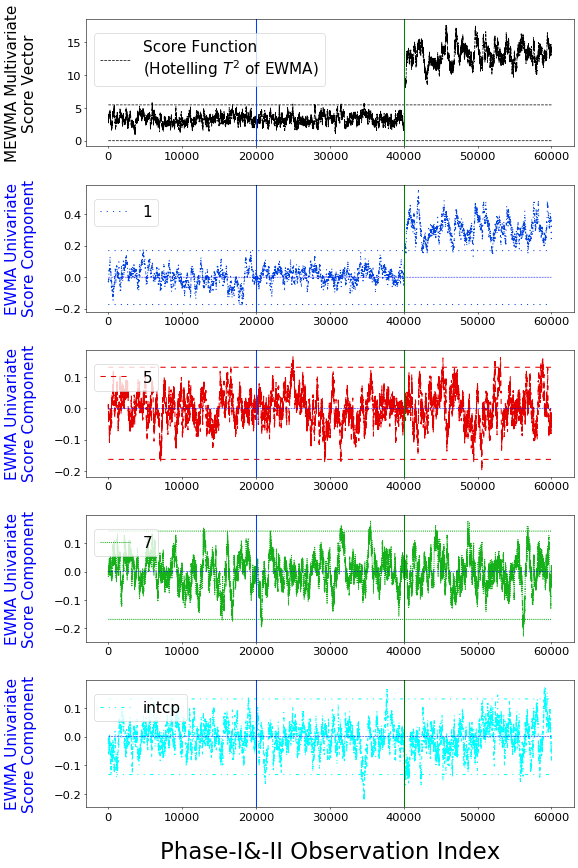
\includegraphics[width = 0.55\linewidth]{./figures_archive/sim_2/reg/neg_single_1_sim2_mlines_with_regu_1e-08_0_005.png}
  \caption{An abrupt concept drift in the linear model with independent covariates. For conciseness, here we only show score-based MEWMA and the component EWMA control charts for the $\theta_1$, $\theta_5$, $\theta_7$, and $\theta_0$~(bottom plots). The $1$st~(blue) and $2$nd~(green) vertical lines mark the boundaries of Phase-I/II and before/after the concept drift, respectively.}
  \label{fig_CD:lin_reg_ind_X}
\end{figure}

\subsection{Abrupt Concept Drift with Correlated Covariates}
\label{ssss_CD:lin_not_ind_pred}
To introduce multicolinearity, which is common in real data sets, we continue the example of Appendix~\ref{ssss_CD:lin_ind_pred} but modify the covariates via $x_5 \leftarrow 0.5 x_1 + 0.5 x_5$ and $x_6 \leftarrow 0.3 x_1 + 0.3 x_2 + 0.4 x_6$ without modifying the other covariates. The MEWMA and component EWMA control charts before and after the Fisher decoupling by {the inverse of the estimated} $\widetilde{\mathbb {I}}(\bm { \theta}^{(0)})$ are shown in Figure~\ref{fig_CD:lin_reg_not_ind_X}. We see that if we do not apply the Fisher decoupling, parameters with no concept drift can appear to have experienced drift if their corresponding covariates are correlated with other covariates. For example, in the left plots~(component EWMA control charts without Fisher decoupling) $\theta_5$ appears to drift even though it did not change, because $x_5$ is correlated with $x_1$ and $\theta_1$ did change. In contrast, the right plots~(component EWMA control charts for the Fisher-decoupled scores) correctly show that $\theta_1$ changed but $\theta_5$ did not.

\begin{figure}[!htbp]
\centering
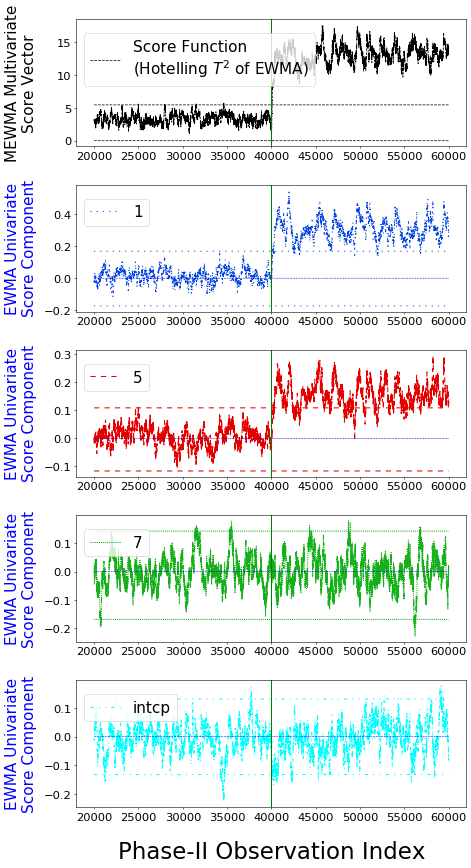
\includegraphics[width = 0.4\linewidth]{./figures_archive/sim_4/reg/PII_neg_single_1_sim4_mlines_with_regu_1e-08_0_005.png}
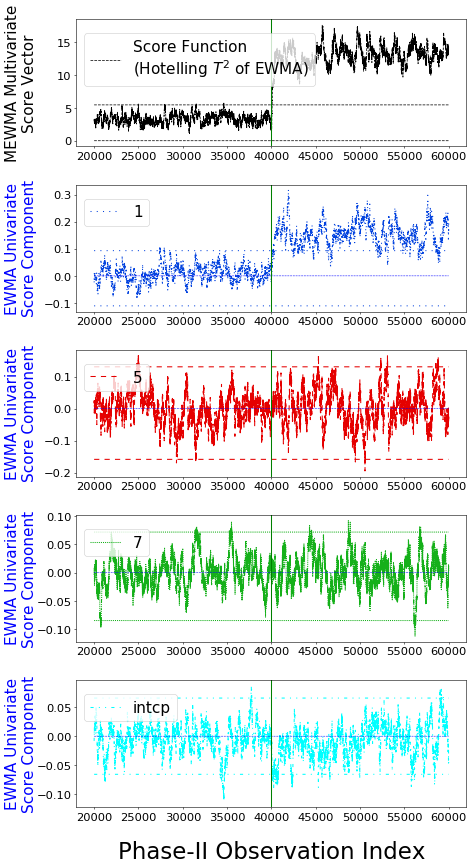
\includegraphics[width = 0.4\linewidth]{./figures_archive/sim_4/reg/PII_neg_single_1_sim4_fisher_mlines_with_regu_1e-08_0_005.png}
\caption{Illustration of the importance of Fisher decoupling with correlated covariates. The left plots are the score-based MEWMA and various component EWMA control charts without Fisher decoupling, and the right plots are the same but with Fisher decoupling. The former indicates that $\theta_5$ changed, whereas the latter correctly indicates that it did not.
}
  \label{fig_CD:lin_reg_not_ind_X}
\end{figure}

\subsection{Gradual Concept Drift with Correlated Covariates}
\label{ssss_CD:lin_not_ind_pred_grad_cd}
In real applications, concept drift often occur gradually. In this example, all conditions are the same with those in Appendix~\ref{ssss_CD:lin_not_ind_pred} except that parameters change linearly, instead of abruptly, over the second half of Phase-II. Figure~\ref{fig_CD:lin_reg_not_ind_X_grad_cd} shows the score-based MEWMA and component EWMA control charts with and without Fisher decoupling. As in Figure~\ref{fig_CD:lin_reg_not_ind_X}, the component EWMA control charts for the Fisher-decoupled scores~(the right column) correctly indicate that $\theta_1$ changed gradually and $\theta_5$ did not change, whereas the component EWMA control charts for the undecoupled scores~(the left column) conflate the two.

\begin{figure}[!htbp]
\centering
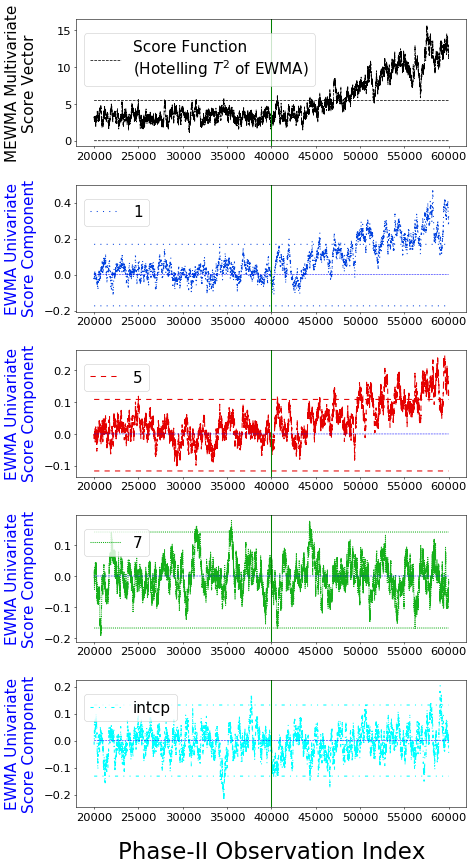
\includegraphics[width = 0.4\linewidth]{./figures_archive/sim_6/reg/PII_neg_single_1_sim6_mlines_with_regu_1e-08_0_005.png}
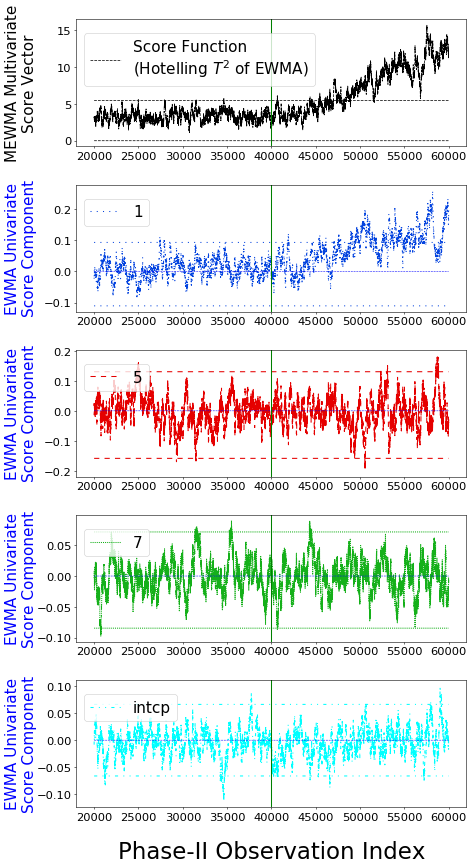
\includegraphics[width = 0.4\linewidth]{./figures_archive/sim_6/reg/PII_neg_single_1_sim6_fisher_mlines_with_regu_1e-08_0_005.png}
\caption{Score-based monitoring and diagnostic results analogous to Figure~\ref{fig_CD:lin_reg_not_ind_X} but with gradual~(instead of abrupt) concept drift. Illustration of the importance of Fisher decoupling with correlated covariates. As in Figure~\ref{fig_CD:lin_reg_not_ind_X}, the Fisher-decoupled component EWMA control charts~(the right column) correctly indicate that $\theta_1$ changed but $\theta_5$ did not.}
  \label{fig_CD:lin_reg_not_ind_X_grad_cd}
\end{figure}
\end{appendices}

\bibliography{sample.bib} % For mac

\end{document}